\documentclass[twoside,english]{uiofysmaster}

\usepackage{pdfpages}
\usepackage{cite}
\usepackage{epsfig}
\usepackage{caption}
\usepackage{subcaption}
\usepackage[normalem]{ulem}
\usepackage{textcomp}
\usepackage{varioref}

%\bibliography{references}

\author{J\o rgen Eriksson Midtb\o}
\title{Noe}
\date{June 2015}

\begin{document}

\pagenumbering{roman}
\includepdf{front-page.pdf}
\cleardoublepage

\begin{abstract}
This is an abstract text.
\end{abstract}

%\begin{dedication}
%  Til Nina Eriksson
%  \\\vspace{12pt}
%  This is a dedication
%\end{dedication}

% \begin{acknowledgements}
% Takk til Are Raklev for god rettleiing, til Lars Dal og Anders Kvellestad for god hjelp, og til Anders Lauvland og Anders Hafreager for gode diskusjonar. Takk til Janne for at du er du. Takk til pappa. Takk også til Bryan Webber, Mona Semb, Tor Gjerrestad, Arild [], 
% \end{acknowledgements}

\tableofcontents
\listoffigures
\listoftables



%%%%%%%%%%%%%%%%%%%%%%%%%%%%%%%%%%%%%%%%%%%%%%%%%%%%%%%%%%%
\chapter{Supersymmetry}%%%%%%%%%%%%%%%%%%%%%%%%%%%%%%%%%%%%
%%%%%%%%%%%%%%%%%%%%%%%%%%%%%%%%%%%%%%%%%%%%%%%%%%%%%%%%%%%
\label{ch:susyintro}

\marginpar{Should probably include some math}
Supersymmetry is a proposed extension of the Standard model of particle physics. The present chapter gives a brief introduction to the theory of supersymmetry. The summary is largely based on \cite{Batzing:2013}.

\section{The Standard Model of Particle Physics}
The standard model of particle physics has been hugely successful in explaining what our universe consists of and how the constituents interact with each other. But it is well known that the standard model is incomplete, for instance since it gives no explanation for dark matter. There are also more technincal problems with the standard model, such as the hierarchy problem of the Higgs boson mass loop corrections and the arbitrariness of the model parameters.

\begin{itemize}
	\item Do the following section more mathematically. Introduce the general ingredients of a gauge theory: Gauge groups, transformations, covariant derivatives and fields. Representations. This also facilitates the discussion of the super-symmetry later by analogy.
\end{itemize}

The standard model is a quantum field theoretic model, and may be stated in terms of a Lagrangian density function $\mathcal{L}$. The guiding principle for constructing the Lagrangian is {\it gauge invariance}. Gauge degrees of freedom are degrees of freedom which are ``superflous'', in the sense that they do not have any observable consequences. This is exploited by requiring that the Lagrangian, which determines the physical dynamics, does not change when the gauge degrees of freedom are varied -- the Lagrangian is gauge invariant.

The standard model consists of three Lie groups of quadratic matrices, the infamous $U(1)_Y\times SU(2)_L\times SU(3)_C$. The number in the parenthesis gives the matrix dimension of the group. The symbols $U$ and $SU$ stand for {\it unitary} and {\it special unitary}, respectively. Unitary means that the matrices are unitary, and special means they have determinant 1. The groups are Lie groups, which means that they are continuous, and thus that any transformation of a group element may be constructed from infinitesimal transformations. The objects on which the group acts may be given in several {\it representations}. In the case of matrix groups this means vectors of different dimension. For an $SU(n)$ group, the two most important representations are the {\it fundamental} representation, where the vectors have dimension $n$, and the {\it adjoint} representation, where the vectors have dimension $n^2-1$. 

A transformation by a group element may generally be written as 
\begin{align}
	\exp(something sum of generators),
\end{align}
where $T_a$ are called the generators of the Lie algebra corresponding to the group. The generators themselves are in the fundamental representation represented by $n^2-1$ traceless complex $n\times n$ matrices -- for $SU(2)$, these are the Pauli matrices $\sigma_i$, and for $SU(3)$ they are the Gell-Mann matrices $\lambda_i$ -- and in the adjoint representation by the {\it structure coefficients} $f_{abc}$ as $(T_a)_{bc} = f_{abc}$. The structure coefficients are determined from the Lie algebra as
\begin{align}
	[T_a, T_b] = i f_{abc}T_c,
\end{align}
where repeated indices are summed over.

The standard model is a quantum field theoretic model and may be stated in terms of a Lagrangian density function $\mathcal{L}$. The features that define the standard model emerge by requiring that it is invariant under the action of certain {\it gauge groups} -- specifically the infamous $U(1)_Y\times SU(2)_L\times SU(3)_C$, where the subscripts stand for {\it hypercharge, left} and {\it colour}, respectively, and refer to the properties that the different fields must have in order to be acted upon by the group transformations. By inserting certain {\it fermionic} field content in the Lagrangian and imposing these symmetries, the model acquires a number of {\it gauge bosons} for the different gauge groups. All these particles are {\it a priori} massless, a requirement to fulfill the gauge symmetry. To give particles their observed mass, then, one adds a scalar field and a corresponding scalar potential of a certain shape. The shape of the potential is such that the $U(1)_Y\times SU(2)_L$ symmetry is {\it spontaneously broken} at a certain energy scale, shifting the degrees of freedom around to give a scalar Higgs boson along with the other gauge bosons, and also giving mass to all particles except the photon. The remaining unbroken symmetries are then the $U(1)_\mathrm{em}$ for electromagnetic and $SU(3)_C$ for strong interactions. 

The particles that make up the standard model are: the three generations of charged leptons, electron, muon and tau, and their three neutral counterparts, the neutrinos; the three generations of up- and down-type quarks up, down, charm, strange, top and bottom; the electroweak gauge bosons photon, Z and W; the strong gauge bosons, the gluons; and the Higgs boson. 

\section{Motivations for extending the standard model}
\begin{itemize}
	\item Dark matter
	\item Also other things? Neutrino masses (although not explained)? EWSB? Hierarchy problem? 
\end{itemize}

As mentioned, one of the big problems with the standard model is that is has no candidate for particle dark matter. Observations over the last century have given strong evidence for the existence of some as yet unkown form of matter which is distributed in large quantites all over the universe -- in fact four times as much as our ordinary matter. It is widely believed that this dark matter is some form of particle. Dark matter interacts primarily, or possibly even solely, via gravitation, so the particle has to be colourless and electrically neutral, because the strength of these interactions would lead to the particle having been observed by now. It also has to be long-lived in order to explain the abundance of dark matter that we observe in the universe today, because the assumption is that it was thermally produced in the early universe and subsequently cooled off. These restrictions rule out most of the standard model particles, with the exception of neutrinos. But neutrinos are known to be very light, almost massless, and calculations of early-universe dynamics show that they are too light to be candidates for dark matter. 

\section{Extending the standard model by supersymmetry}
Supersymmetry is a proposed extension of the standard model which increases the number of degrees of freedom by introducing a symmetry between fermions and bosons. The construction of supersymmetry is in some sense a two-step process, where one first derives the Lagrangian of a theory with complete symmetry between fermions and bosons, meaning that every bosonic degree of freedom gets a corresponding `supersymmetric' fermionic degree of freedom, and {\it vice versa}. These fields only differ in spin. But since we have not observed {\it e.g.\ } scalar, colour charged particles with the same mass as the quarks, the symmetry can not be exact. To make the theory physically viable, the supersymmetric partners must be significantly heavier than their standard model counterparts. 


\subsection{Lagrangian content, superfields}
\begin{itemize}
	\item Two main types: Chiral and vector supermultiplets.
\end{itemize}

\subsection{SUSY breaking}




\section{The Minimal Supersymmetric Standard Model}
\subsection{R-parity}
\begin{itemize}
	\item Needed to make the proton stable; DM is a great side effect
\end{itemize}

\subsection{Renormalization group equation}
\begin{itemize}
	\item Include plot from Stephen Martin. 
\end{itemize}

\begin{figure}
	\centering
	\includegraphics[width=0.8\textwidth]{figures/susyintro/MSSMrun.eps}
	\caption{MSSM RGE running, from \cite{Martin:1997ns}.}
	\label{fig:mssm_rgerun}
\end{figure}



























%%%%%%%%%%%%%%%%%%%%%%%%%%%%%%%%%%%%%%%%%%%%%%%%%%%%%%%%%%%%%%%%%%%%%%%%%%%
\chapter{Determination of SUSY particle masses from cascade decays}%%%%%%%%
%%%%%%%%%%%%%%%%%%%%%%%%%%%%%%%%%%%%%%%%%%%%%%%%%%%%%%%%%%%%%%%%%%%%%%%%%%%
\label{ch:introducing_the_method}


\marginpar{Separate into introduction chapter}
In the following chapters we will present and discuss a method for determining the masses of supersymmetric particles in certain types of cascade decays. The present chapter formulates the type of process we are studying and the problems we face, and presents a novel method proposed by B. Webber \cite{Webber:2009vm} for making inferences about the unknown masses. The subsequent chapters deal with investigation and improvements on the method. We begin by simulating events, adding complexities layer by layer, investigating the method and getting some feeling for its aptitude. We then discuss some problems with the original formulation, suggest ways to amend these and look at ways to develop the method further.

\section{The problem}
Consider an LHC event where two chains of the form
\begin{align}
	\tilde{q} \to q + \tilde{\chi}_2^0, \, \tilde{\chi}_2^0 \to l^{\pm} + \tilde{l}^\mp, \, \tilde{l}^\mp \to l^\mp + \tilde{\chi}_1^0\label{eq:goldencascade}
\end{align}
are present. Combined, the measurable particles in the two chains are the two quarks and four leptons, where the lepton pairs are opposite-sign same-flavour. The LSPs escape detection, but the sum of their transverse momenta can be measured as the missing $p_T$. The quantities of interest, however, are the masses of the supersymmetric particles, $m_{\tilde{q}}, m_{\tilde{\chi}_2^0}, m_{\tilde{l}}$ and $m_{\tilde{\chi}_1^0}$. (Potentially with several values for the squarks and sleptons if they differ in generation between the sides.) These are not directly measurable, but the kinematics of the problem depend on them. 

Many methods have been investigated for the purpose of measuring supersymmetric masses \cite{Barr:2010zj}. One well known example is the end-point method \cite{1126-6708-2000-09-004}. We measure {\it e.g.}\ the dilepton invariant mass in the process \eqref{eq:goldencascade}. The distribution of the dilepton invariant mass can be shown to form a right triangle where the maximal value is given by
\begin{align}
	(m_{ll}^\mathrm{max})^2 = \frac{ \left( m^2_{\tilde{\chi}_2^0} - m^2_{\tilde{l}} \right) \left( m^2_{\tilde{l}} - m^2_{\tilde{\chi}_1^0} \right)}{m^2_{\tilde{l}}}, \label{eq:invariant_mass_endpoint}
\end{align}
thus constraining $m_{\tilde{\chi}_2^0}$, $m_{\tilde{l}}$ and $m_{\tilde{\chi}_1^0}$. Similar constraints may be obtained for the three other visible particle combinations, giving four equations with four unknowns. This method is very dependent on statistics, since each measured event only contributes one point to the distribution. A large number of events is required to get a reliable value. However, the number of events contributing to the measurement is also much larger, since each side of the decay chain contribute individually, thus making use of events with leptons on one side only as well.



\section{Webber's method}
Webber \cite{Webber:2009vm} suggests a different method, where all available kinematical info from every event is used. Consider the general decay tree in figure \ref{fig:decaytree}. We assume that we have an event with two such chains, but not necessarily with identical particles in the two. We will distinguish the two chains by referring to them as the <<first>> and <<second>> one, although the assignment is arbitrary.
\begin{figure}[hbt]
\centering
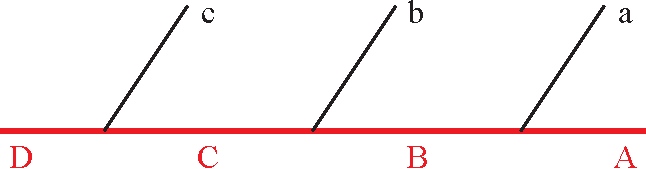
\includegraphics[scale=0.7]{figures/fig-chain.pdf} % Stolen!
\caption{Decay topology.}
\label{fig:decaytree}
\end{figure}
Assuming that the decaying particles are on-shell, the four-momenta in the first chain should satisfy
\begin{align}
	(p_c + p_b + p_a + p_A)^2 &= M_D^2,\nonumber \\
	(p_b + p_a + p_A)^2 &= M_C^2,\nonumber \\
	(p_a + p_A)^2 &= M_B^2,\label{eq:constraints}\\
	p_A^2 &= M_A^2.\nonumber
\end{align}
The first three equations give three linear constraints on the invisible four-momentum $p_A$:
\begin{align}
	-2p_c\cdot p_A &= M_C^2 - M_D^2 + 2p_c\cdot p_b + 2p_c \cdot p_a + m_c^2 \equiv S_1,\nonumber \\
	-2p_b\cdot p_A &= M_B^2 - M_C^2 + 2p_b\cdot p_a + m_b^2 \equiv S_2,\\
	-2p_a\cdot p_A &= M_A^2 - M_B^2 + m_a^2 \equiv S_3. \nonumber
\end{align}
Equivalently the second chain (with primed indices) gets the constraints
\begin{align}
	-2p_{c'}\cdot p_{A'} &= M_{C'}^2 - M_{D'}^2 + 2p_{c'}\cdot p_{b'} + 2p_{c'} \cdot p_{a'} + m_{c'}^2 \equiv S_5,\nonumber \\ 
	-2p_{b'}\cdot p_{A'} &= M_{B'}^2 - M_{C'}^2 + 2p_{b'}\cdot p_{a'} + m_{b'}^2 \equiv S_6,\\
	-2p_{a'}\cdot p_{A'} &= M_{A'}^2 - M_{B'}^2 + m_{a'}^2 \equiv S_7.\nonumber
\end{align}
In addition we have the transverse momentum constraints
\begin{align}
	p_A^x + p_{A'}^x &= p_\mathrm{miss}^x \equiv S_4, \label{eq:Svec_orig} \\
	p_A^y + p_{A'}^y &= p_\mathrm{miss}^y \equiv S_8. \nonumber
\end{align}

The vector $\mathbf{S} = (S_1, S_2, ...)$ thus depends on the eight unknown masses 
\begin{align}
	\mathbf{M} = (M_D^2, M_C^2, M_B^2, M_{A'}^2, M_{D'}^2, M_{C'}^2, M_{B'}^2, M_{A'}^2)
\end{align}
and the visible momenta which in principle are measurable. We define a vector containing the four-momenta of the invisible final state particles as
\begin{align}
	\mathbf{P} = (p_A^x, p_A^y, p_A^z, E_A, p_{A'}^x, p_{A'}^y, p_{A'}^z, E_{A'}). \label{eq:Pvec}
\end{align}
We then have
\begin{align}
	\mathbf{A}\mathbf{P} = \mathbf{S},\label{eq:APS}
\end{align}
where
\begin{align}
	\mathbf{A} = 2 \begin{pmatrix}
						p_c^x & p_c^y & p_c^z & -E_c & 0 & 0 & 0 & 0 \\
						p_b^x & p_b^y & p_b^z & -E_b & 0 & 0 & 0 & 0 \\
						p_a^x & p_a^y & p_a^z & -E_a & 0 & 0 & 0 & 0 \\
						1/2 & 0 & 0 & 0 & 1/2 & 0 & 0 & 0\\
						0 & 0 & 0 & 0 & p_{c'}^x & p_{c'}^y & p_{c'}^z & -E_{c'} \\
						0 & 0 & 0 & 0 & p_{b'}^x & p_{b'}^y & p_{b'}^z & -E_{b'} \\
						0 & 0 & 0 & 0 & p_{a'}^x & p_{a'}^y & p_{a'}^z & -E_{a'} \\
						0 & 1/2 & 0 & 0 & 0 & 1/2 & 0 & 0
					\end{pmatrix}. \label{eq:Amatrix_orig}
\end{align}
Furthermore, $\mathbf{S}$ may be written as 
\begin{align}
	\mathbf{S} = \mathbf{B} \mathbf{M} + \mathbf{C},\label{eq:SBMC}
\end{align}
where
\begin{align}
	\mathbf{B} = \begin{pmatrix}
					-1 & 1 & 0 & 0 & 0 & 0 & 0 & 0 \\
					0 & -1 & 1 & 0 & 0 & 0 & 0 & 0 \\
					0 & 0 & -1 & 1 & 0 & 0 & 0 & 0 \\
					0 & 0 & 0 & 0 & 0 & 0 & 0 & 0 \\
					0 & 0 & 0 & 0 & -1 & 1 & 0 & 0 \\
					0 & 0 & 0 & 0 & 0 & -1 & 1 & 0 \\
					0 & 0 & 0 & 0 & 0 & 0 & -1 & 1 \\
					0 & 0 & 0 & 0 & 0 & 0 & 0 & 0 \\
	\end{pmatrix}
\end{align}
and
\begin{align}
	\mathbf{C} = ( &2p_c \cdot p_b + 2p_c \cdot p_a + m_c^2, 2 p_2 \cdot p_3 + m_b^2, m_a^2, p_\mathrm{miss}^x, \nonumber \\ 
				   &2p_{c'}\cdot p_{b'} + 2 p_{c'} \cdot p_{a'} + m_{c'}^2, 2 p_{b'} \cdot p_{a'} + m_{b'}^2, m_{a'}^2, p_\mathrm{miss}^y )
\end{align}
With all this, the solution for the invisible four-momenta, given the unknown masses, is 
\begin{align}
	\mathbf{P} = \mathbf{A}^{-1} \mathbf{S} = \mathbf{D} \mathbf{M} + \mathbf{E},
\end{align}
where $\mathbf{D} = \mathbf{A}^{-1}\mathbf{B}$ and $\mathbf{E} = \mathbf{A}^{-1}\mathbf{C}$.

The matrix $\mathbf{D}$ and vector $\mathbf{E}$ contain only measurable quantities, hence they only need to be calculated once for every event. For the true value of the unknown masses $\mathbf{M}$, the system should satisfy the on-shell conditions
\begin{align}
	p_{A}^2 &= P_4^2 - P_1 ^2 - P_2^2 - P_3^2 = M_{A}^2, \nonumber\\
	p_{A'}^2 &= P_8^2 - P_5 ^2 - P_6^2 - P_7^2 = M_{A'}^2.
\end{align}
So by calculating $\mathbf{D}_n$ and $\mathbf{E}_n$ for each event $n$, and making a {\it hypothesis} $\mathbf{M}$ for the unknown masses, we can measure the goodness of fit for our hypothesis by the quantity
\begin{align}
	\xi^2(\mathbf{M}) = \sum_n \left[(p_{A}^2)_n - M_A^2\right]^2 + \left[(p_{A'}^2)_n - M_{A'}^2\right]^2. \label{eq:xisquared}
\end{align}
Note that this quantity measures the goodness-of-fit of all the unknown masses equally, since it follows from the constraint equations \eqref{eq:constraints} that {\it e.g.}
\begin{align}
	(p_B^2)_n - M_B^2 &= (p_a + p_A)_n^2 - M_B^2 = \nonumber\\
				  &= (p_a^2)_n + (p_A^2)_n + 2p_a\cdot p_A - M_B^2\nonumber\\
				  &= (p_a^2)_n + (p_A^2)_n - M_A^2 + M_B^2 - m_a^2 - M_B^2\\
				  &= (p_A^2)_n - M_A^2.\nonumber
\end{align}

For each event there are eight constraining equations. There are eight unknowns from the masses plus six from the unknown LSP momenta (using the on-shell constraint on the LSPs). The system is thus underconstrained, with six free parameters. The point of the method is to minimize $\xi^2$ as a function of $\mathbf{M}$. This is generally an eight-dimensional minimization problem with a potentially very complicated function, and thus not easy to solve. However, in the case of identical chains, it reduces to a much more handleable four-dimensional one which one could hope could be solved. In this case the number of free parameters reduces from six to two. The condition of identical chains can often be satisfied by a combination of vetoing ({\it e.g.} b-jets) and assuming small mass splittings between different generations, thus approximating their masses as equal. This is a realistic assumption in many SUSY scenarios.\marginpar{Refer to previous chapter about SUSY}

\section{Two technical modifications}\label{sec:dimension_fixing}
The aptness of the method hangs on the invertibility of the matrix $\mathbf{A}$.\marginpar{Does it really hang on it?} However, the matrix as it stands in \eqref{eq:Amatrix_orig}, is technically ill-defined for inversion since not all rows have the same units. The rows 4 and 8, corresponding to the components 4 and 8 of the vector $\mathbf{S}$ \eqref{eq:Svec_orig}, have no dimension, while the other rows have dimension $(\mathrm{mass})^1$. This is reflected in the components of $\mathbf{S}$, which all except 4 and 8 have dimension $(\mathrm{mass})^2$. This means both that the magnitude of the determinant is sensitive to the choice of mass scale (since some rows have non-zero dimension) and that it does not scale properly for numerical calculations (since not all rows have the same dimension). This is something that Webber does not comment on (and the method still in principle works), but we make some minor reformulations of the method in order to amend both problems.

For the first, we redefine $S_4$ and $S_8$ to be 
\begin{align}
	S_4 &\equiv (p_A^x + p_{A'}^x)^2 = (p_\mathrm{miss}^x)^2, \label{eq:Svec_modified} \\
	S_8 &\equiv (p_A^y + p_{A'}^y)^2 = (p_\mathrm{miss}^y)^2. \nonumber
\end{align}
We do not wish to redefine $\mathbf{P}$ \eqref{eq:Pvec}, so to keep the relationship $\mathbf{S} = \mathbf{A}\mathbf{P}$ we modify rows 4 and 8 of $\mathbf{A}$ to
\begin{align}
	\mathbf{A}_4 &= (p_\mathrm{miss}^x, 0, 0, 0, p_\mathrm{miss}^x, 0, 0, 0),\\
	\mathbf{A}_8 &= (0, p_\mathrm{miss}^y, 0, 0, 0, p_\mathrm{miss}^y, 0, 0),\nonumber
\end{align}
such that $\mathbf{A}$ now is
\begin{align}
	\mathbf{A} = 2 \begin{pmatrix}
						p_c^x & p_c^y & p_c^z & -E_c & 0 & 0 & 0 & 0 \\
						p_b^x & p_b^y & p_b^z & -E_b & 0 & 0 & 0 & 0 \\
						p_a^x & p_a^y & p_a^z & -E_a & 0 & 0 & 0 & 0 \\
						p_\mathrm{miss}^x/2 & 0 & 0 & 0 & p_\mathrm{miss}^x/2 & 0 & 0 & 0\\
						0 & 0 & 0 & 0 & p_{c'}^x & p_{c'}^y & p_{c'}^z & -E_{c'} \\
						0 & 0 & 0 & 0 & p_{b'}^x & p_{b'}^y & p_{b'}^z & -E_{b'} \\
						0 & 0 & 0 & 0 & p_{a'}^x & p_{a'}^y & p_{a'}^z & -E_{a'} \\
						0 & p_\mathrm{miss}^y/2 & 0 & 0 & 0 & p_\mathrm{miss}^y/2 & 0 & 0
					\end{pmatrix}. \label{eq:Amatrix_modified}
\end{align}

This redefinition does not alter the solvability of the problem, since the only information lost in $\mathbf{S}$ is the sign of $p_\mathrm{miss}^i$ which is kept in $\mathbf{A}$ instead. Also it keeps the essential feature that $\mathbf{A}$ only contains measured quantities, so that it can be inverted prior to making a mass hypothesis. The redefinition of $\mathbf{S}$ means we also have to modify $\mathbf{C}$ to keep the relationship $\mathbf{S} = \mathbf{B} \mathbf{M} + \mathbf{C}$ (from eq.\ \eqref{eq:SBMC}). We thus make the same redefinitions here, {\it i.e.}
\begin{align}
	C_4 &\equiv (p_\mathrm{miss}^x)^2, \label{eq:Cvec_modified} \\
	C_8 &\equiv (p_\mathrm{miss}^y)^2. \nonumber
\end{align}

The other issue is to make the numerical problem dimensionless. All elements of $\mathbf{A}$ and $\mathbf{P}$ now have mass dimension 1, while all elements of $\mathbf{S}$, and thus $\mathbf{M}$ and $\mathbf{C}$, have dimension 2. We are free to multiply both sides of eq.\ \eqref{eq:APS} by some normalization mass $M_\mathrm{norm}$ squared,
\begin{align}
	\frac{1}{M_\mathrm{norm}^2} \mathbf{A}\mathbf{P} = \frac{1}{M_\mathrm{norm}^2} \mathbf{S},
\end{align}
and we choose to take it into the matrix and vectors such that they all become dimensionless, {\it i.e.}\ we modify
\begin{align}
	\mathbf{\hat A} = \frac{1}{M_\mathrm{norm}}\mathbf{A},\nonumber \\
	\mathbf{\hat P} = \frac{1}{M_\mathrm{norm}}\mathbf{P},\label{eq:vectors_normalized}\\
	\mathbf{\hat S} = \frac{1}{M_\mathrm{norm}^2}\mathbf{S},\nonumber 
\end{align}
thus modifying $\mathbf{M}$ and $\mathbf{C}$ in the same way as $\mathbf{S}$ to comply with eq.\ \eqref{eq:SBMC}. We also modify the fitting function $\xi^2$ accordingly, so that it becomes
\begin{align}
	\xi^2(\mathbf{M}) = \sum_n \left[(\hat p_{A}^2)_n - \frac{M_A^2}{M_\mathrm{norm}^2}\right]^2 + \left[(\hat p_{A'}^2)_n - \frac{M_{A'}^2}{M_\mathrm{norm}^2}\right]^2.\label{eq:xisquared_modified}
\end{align}

To obtain numbers of order one, which is optimal for numerical purposes, we should pick a mass of the relevant scale for the problem. This is not something that is known {\it a priori}, since it depends on the supersymmetric masses that we are trying to determine. We might be tempted to use something based on the measured momenta, but this is a bad idea since it would mean weighting different events differently. We choose the normalization constant
\begin{align}
	M_\mathrm{norm} = 100 \,\mathrm{GeV},
\end{align}
the same order of magnitude as we expect for the supersymmetric masses ($\sim$ electroweak scale). 

We have made thorough checks that this formulation and the original one produce identical results within numerical accuracy, so that indeed the formulations are equivalent.









\section{Taking account of combinatorics}
\label{sec:combinatorics}
In a real detector event, the ordering of the quarks and leptons in and between chains is not known -- all we have are the measured particle types and their momenta. We must take this into account when applying the method to Monte Carlo simulated datasets. Webber does this by evaluating all possible combinations in each event at each mass point and selecting the combination which gives the lowest $\xi^2$ value, choosing to add this value to the sum in eq.\ \eqref{eq:xisquared_modified}. The number of possible combinations are 8 or 16, depending on whether the lepton pairs in the two chains are the same flavour or not. 

For two pairs of different-generation leptons, the possible orderings are (given some `base ordering' which we permute from): Switching the ordering of the leptons in the first chain; switching the ordering of the leptons in the second chain; or switching the leptons in both chains. For each of these permutations we have the option to switch the two quarks, so the total number of combinations is 8. In the case of identical leptons, we may additionally interchange leptons between the chains -- but this only increases the total combinations by a factor of 2 because the same-chain leptons must have opposite charge.

Note that in order to switch the ordering of leptons within the same chain, all we need to do is permute the rows of the matrix $\mathbf{A}$. The vector $\mathbf{C}$ is invariant as long as the same-chain leptons have the same mass. When the quarks are flipped, however, or when leptons are interchanged between chains, then we must redefine $\mathbf{A}$ and $\mathbf{C}$. Webber makes a point that this property can save computer memory, since one only has to store two or four versions of the matrix and vector for each event. We have not found this to be an issue.












\section{Outline of the plan}
\marginpar{Better reformulate away from ``reproduce'', and also modify to be what I actually do}
In this thesis we wish to investigate and develop this method further. We will begin by trying to reproduce Webber's parton level results using Monte Carlo simulations. We will then add layers of realism and complexety approaching something closer to the real experimental situation, in order to investigate its full potential. In the end we will focus on well motivated scenarios that can be discovered in Run II of the LHC.  Along the way we will also make some improvements on the method.

The plan of attack is as follows:
\begin{enumerate}
	\item We begin by generating squark pairs at rest, decaying them in the chain of on-shell two-body decays given in (\ref{eq:goldencascade}). The visible decay products, quarks and leptons, are then used to reconstruct the masses. As a benchmark we investigate the precision attainable for the parameter point SPS1a~\cite{Allanach:2002nj}, which was used by Webber. 
	\item Because of final state radiation and parton showering, as well as---to a lesser degree---sparticle widths, the particles in the decay chain will not be on-shell due to extra gluons (and photons) in the final state. We employ a more sophisticated Monte Carlo code, {\tt Herwig++}~\cite{Bahr:2008pv}  to simulate these properties. This should have an effect on the mass reconstruction since Webber's method assumes on-shell decays.
	\item	We then compare results with and without including the combinatorical issues from identifying the decay products, and we add a simple parametrised momentum smearing, based on realistic detector response, in order to simulate that the measurement of the kinematics of final-state particles is not exact. This was the level of precision employed by Webber in~\cite{Webber:2009vm}.
	\item The partons that emerge from the hadron showers will hadronize, forming a hadron jet before arriving in the detector. Measurement of the initial parton from reconstructing such jets is one of the big challenges of collider physics. We use the {\tt FastJet}~\cite{Cacciari:2011ma} program for jet reconstruction, with algorithms used in the LHC experiments, and study the effect of jet reconstruction on the mass measurement.
	\item In an analysis of real data, one would have to use selection criteria such as cuts on transverse momentum and number of jets and leptons to discriminate between signal and background events. We will apply such cut schemes to our simulated events based on expectations for 14 TeV LHC. In addition we simulate the expected largest backgrounds for a four-lepton supersymmetry search and investigate how the performance of the method is affected by the presence of background.
	\item {\bf If time} As a last step towards realism, we put the events through a fast detector simulation. 
	\item We then investigate improvements over the original model. Webber and collaborators \cite{Nojiri:2010dk} propose combining the kinematical best-fit reconstruction with measurements of end points of invariant mass distributions.
	\item Investigating other types of chains. Not-equal-sided? Different number of steps? Fitting a mass plane rather than points?
	\item Finally, we look at a well motivated model taken from \cite{Allanach:2014gsa} that was constructed on the basis of a small excess seen in 8 TeV data by the CMS Collaboration~\cite{CMS:2014jfa}, which would be consistent with the decay chain in (\ref{eq:goldencascade}). We show what precission we can expect from mass measurments at 14 TeV LHC should such a scenario be realized.
\end{enumerate}






























%%%%%%%%%%%%%%%%%%%%%%%%%%%%%%%%%%%%%%%%%%%%%%%%%
\chapter{Investigating Webber's method by Monte Carlo simulations}
\label{ch:MC}
%%%%%%%%%%%%%%%%%%%%%%%%%%%%%%%%%%%%%%%%%%%%%%%%%
Webber demonstrates the aptitude of the method on a Monte Carlo generated dataset. A natural starting point for our study is to try to reproduce his results. 

\section{Collider physics}
There are several ways in which a pair of squarks can be produced in $pp$ collisions. The three main categories are: direct pair production of two squarks or a squark-antisquark pair; squark plus gluino with subsequent gluino decay to a squark; and pair production of two gluinos which both subsequently decay to squarks. The mechanism of production affects how much momentum goes into the squark, and thus the momentum of the subsequent decay chain. But our method deals mainly with the internal kinematics of the squark decay, which by Lorentz invariance is independent of squark momentum. The only variables in our analysis which explicitly depends on the overall event kinematics is the missing transverse momentum. The three different categories also determine how many hard jets are present in the event, which affects the combinatorical aspects of reconstructing the chain. This will be discussed in detail later.\marginpar{Better remember to discuss it in detail.}

\section{Reproducing Webber's results}
Webber uses Fortran {\tt HERWIG} version 6.510 \cite{Corcella:2000bw,Moretti:2002eu} to produce events, selecting only events with two left-handed first- or second generation squarks (to limit the mass splitting), but irrespective of the hard production process. The analysis, {\it i.e.} minimization of the $\xi^2$, is performed on 100 samples of 25 events each, using the Minuit {\tt Simplex} \cite{James:1975dr} routine for minimization. He models the effects of measurement errors in a real detector by applying momentum smearing according to a gaussian distribution, and he puts a cut on the total $\xi^2$ obtained at the minimum to eliminate samples which give a bad result. His results are summarized in table 1 of \cite{Webber:2009vm}, which we for convenience show in table \ref{table:webber_original}. 
\begin{figure}[hbt]
	\centering
	\includegraphics[width=0.6\textwidth]{figures/webber_rec_table/sps1a_fits.eps} 
	\caption{fig.\ 2 from \cite{Webber:2009vm}, displayed here for comparison.}
	\label{fig:webber_scatter}
\end{figure}
The column $\delta p/p$ indicates the standard deviation of the gaussian smearing applied on the momenta, $\xi^2_\mathrm{max}$ indicates the cut value of the $\xi^2$, $f_\xi$ is the fraction of samples surviving the cut and $f_\mathrm{cor}$ is the fraction of events where the chosen particle combination, selected as described in section \ref{sec:combinatorics}, is the correct one. 


\begin{table}[hbt]
	\centering
	\begin{tabular}{| l | l | l | l  || l | l | l | l |}
		\hline
		$\delta p/p$ & $\xi^2_\mathrm{max}$ & $f_\xi$ & $f_\mathrm{cor}$ & $m_{\tilde q} (540)$ & $m_{\tilde \chi_2^0} (177)$ & $m_{\tilde l} (143)$ & $m_{\tilde \chi_1^0} (96)$ \\
		\hline \hline
		0 & 	$\infty$ &	100 \%	& 72 \%	& $538 \pm 20$	&	$176 \pm 12$	&	$143 \pm 7$	& 	$95 \pm 10$	\\
		0 &		100 &		80 \%	& 76 \% & $539 \pm 7$	&	$177 \pm 1$		&	$144 \pm 1$	&	$96 \pm 2$	\\
		5 \% &	$\infty$ &	100 \%	& 52 \% & $534 \pm 28$	& 	$176 \pm 11$	&	$143 \pm 10$&	$95 \pm 13$ \\
		5 \% &	100 &		57 \%	& 55 \% & $539 \pm 9$	&	$178 \pm 3$		& 	$144 \pm 2$	&	$96 \pm 4$	\\
		10 \% &	$\infty$ &	100 \%	& 40 \% & $522 \pm 37$	&	$171 \pm 18$	&	$140 \pm 17$&	$88 \pm 26$	\\
		10 \% &	200 &		42 \%	& 43 \% & $530 \pm 22$	& 	$173 \pm 12$	&	$140 \pm 12$&	$89 \pm 20$ \\
		\hline
	\end{tabular}
	\caption{Webber's table of results, taken from table 1 of \cite{Webber:2009vm}.}
	\label{table:webber_original}
\end{table}



% We have made a thorough investigation of these results using a variety of tools. We have generated Monte Carlo events using both Herwig++ 2.7.1  \cite{Bahr:2008pv} and Pythia 8.2 \cite{Sjostrand:2014zea}.\marginpar{Make use of Pythia or don't mention?} We have used the Simplex algorithm in various versions as well as other minimization algorithms for the fit. Webber himself also very generously sent us his own MC generation code, so we were able to make a quite close reconstruction of his analysis. But in the process of confirming his results, we have discovered what appears to be an error in the analysis. The error has to do with the choice of tolerance in the minimization routine. To understand this, we have to briefly discuss the Simplex algorithm.

To reproduce Webber's results, we have generated events using {\tt Herwig++ 2.7.1} \cite{Bahr:2008pv}. As a control, and to enable us to interface the simulation with detector simulation software later, we have also used {\tt Pythia 8.2} \cite{Sjostrand:2014zea}.\marginpar{Remove if I don't do detector simulation.} We have also had access to the code used in the original paper, enabling us to make a quite close reconstruction of Webber's analysis \cite{Webber:epost}. 

To minimize the $\xi^2$ function, we have used the {\tt Simplex} algorithm. We have applied the Minuit version as well as a custom implementation listed in appendix \ref{ch:simplex}. We have discovered that the mass fit is heavily dependent on the input parameters to the {\tt Simplex} minimization, and this makes the fit more challenging. To facilitate the subsequent discussion, we briefly introduce the Simplex method.

\section{The Nelder-Mead Simplex algorithm}

{\tt Simplex} \cite{nelder1965simplex} is a heuristic minimization search method for minimizing a scalar function of $N$ variables. It takes a starting parameter point as input from the user. From this parameter point it erects a {\it simplex}, an ``$N+1$-dimensional triangle''. It then begins to evaluate the function in the vertices of this simplex. A new simplex is constructed by reflecting the vertex with the highest function value around the (hyper)line made out of the other $N$ vertices. Hopefully this new simplex lies lower in the function terrain, and thus the algorithm iterates towards a local minimum. In case of trouble, it may also try contracting the simplex or distorting its shape in various ways to obtain points of lower function values. 

Since the method is heuristic, so is the convergence criterion. Convergence is said to be obtained when the {\it estimated distance to minimum (EDM)} is smaller than some set tolerance value. Usually there is also a predefined maximal number of iterations before the method gives up, to avoid going on forever on non-converging problems. The EDM is defined as
\begin{align}
	\mathrm{EDM}(f_\mathrm{min},f_\mathrm{max}) = \frac{|f_\mathrm{max}-f_\mathrm{min}|}{|f_\mathrm{max}| + |f_\mathrm{min}|},
\end{align}
where $f_\mathrm{min}$ and $f_\mathrm{max}$ are the function values at the lowest and highest point of the current simplex, respectively. This means that the convergence criterion really measures how ``flat'' the simplex is, and thus how steep the function is in the region. If the tolerance is too high, then, we run the risk of obtaining convergence in a region where the gradient is not steep enough to be resolved by the set tolerance, but which may still be far from the minimum.

A pitfall of any minimization routine, also for Minuit Simplex, is that it has a default tolerance value which is used automatically unless the user specifically changes it. The default tolerance in Minuit Simplex is 0.1. This appears to be what Webber has used. We have confirmed that we obtain statistically consistent results when choosing that value. But this does not always resolve this particular function well enough, because it tends to have almost flat directions in mass space for some sets of events.\marginpar{Include $\xi^2$ surface plots. Discuss a bit more?} It therefore leads to convergence at a non-minimal point. If, additionally, the search is started at or close to the masses used to generate the Monte Carlo, then the minimization may obtain ``convergence'' at points very close to the true value, but these points are not minimal points, just regions where the function is not very steep.

\section{The tolerance is too high}

Refer to the scatter plot in fig.\ 2 of \cite{Webber:2009vm}, displayed in fig.\ \ref{fig:webber_scatter} for convenience. This scatter plot shows the fit corresponding to the first row of table \ref{table:webber_original}. We have reproduced this fit using Webber's code \cite{Webber:epost} -- albeit with one modification: Since we don't have access to the old {\tt ISAJET} and {\tt ISAWIG} software for RGE running of SUSY parameters, we have generated our SPS 1a parameter point using {\tt SoftSUSY} version 3.4.1 \cite{Allanach:2001kg}, and converted the resulting SLHA \cite{Skands:2003cj} model file to {\tt ISAWIG} format using the package {\tt PySLHA} version 3.0.2\footnote{We have had to make several modifications to the {\tt PySLHA} code to make the {\tt ISAWIG} output readable by {\tt HERWIG}. These changes have been included in {\tt PySLHA} 3.0.3.} \cite{Buckley:2013jua}. The effects of using a different RGE runner is that the SUSY masses are not exactly the same. The most significant shift is the squarks, which in Webber's case have a mass of 540 GeV, compared to 565 GeV in our case. We observe similar results as Webber gives in his article when we run his code with the original settings for our SUSY parameter point. 
\begin{figure}[hbt]
	\centering
	\begin{subfigure}[b]{0.6\textwidth}
		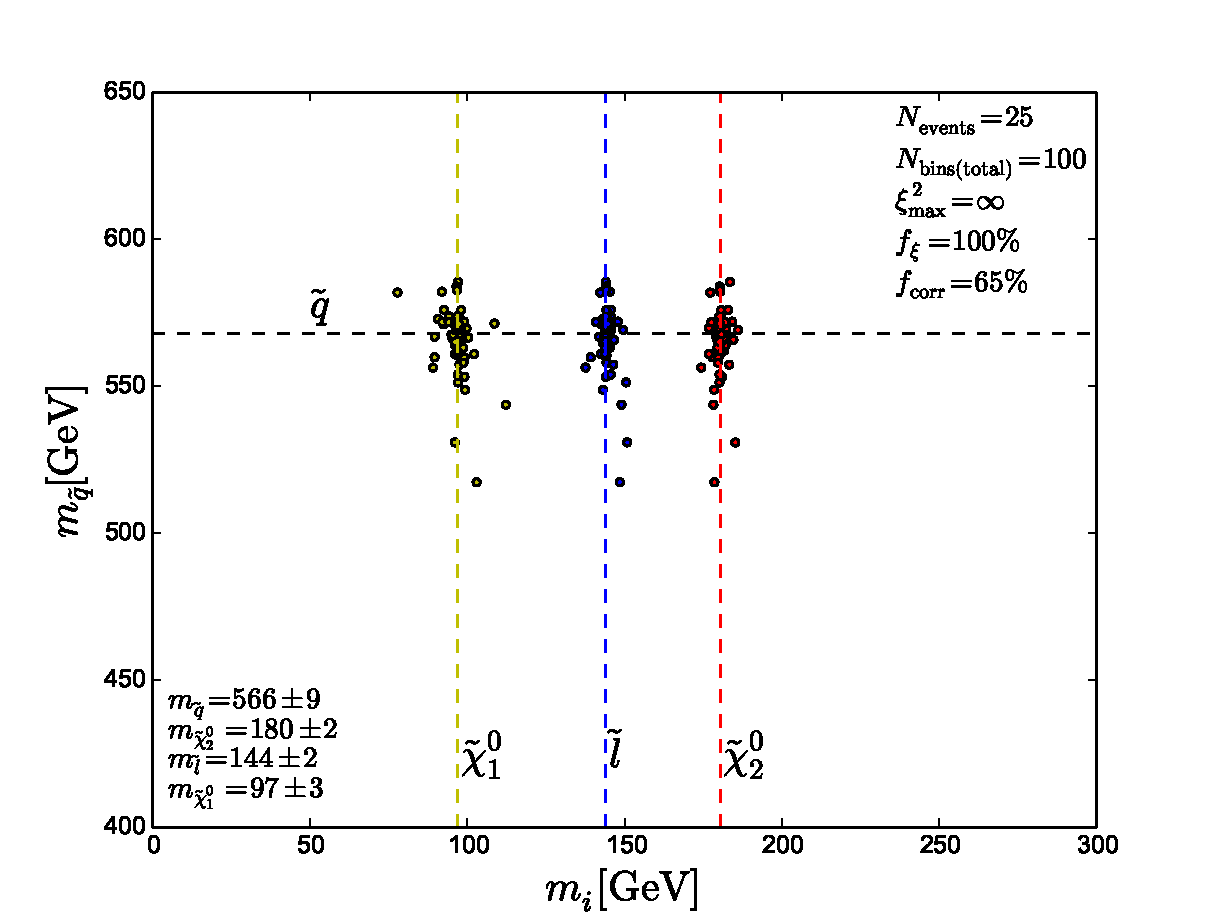
\includegraphics[width=\textwidth]{figures/webber_rec_table/webber_rec_table-samesettings_0psmear-nocut.pdf} 
		\caption{ }
		\label{fig:webber_rec_scatter_tolerance-comparison_a}
	\end{subfigure}

	\begin{subfigure}[b]{0.6\textwidth}
		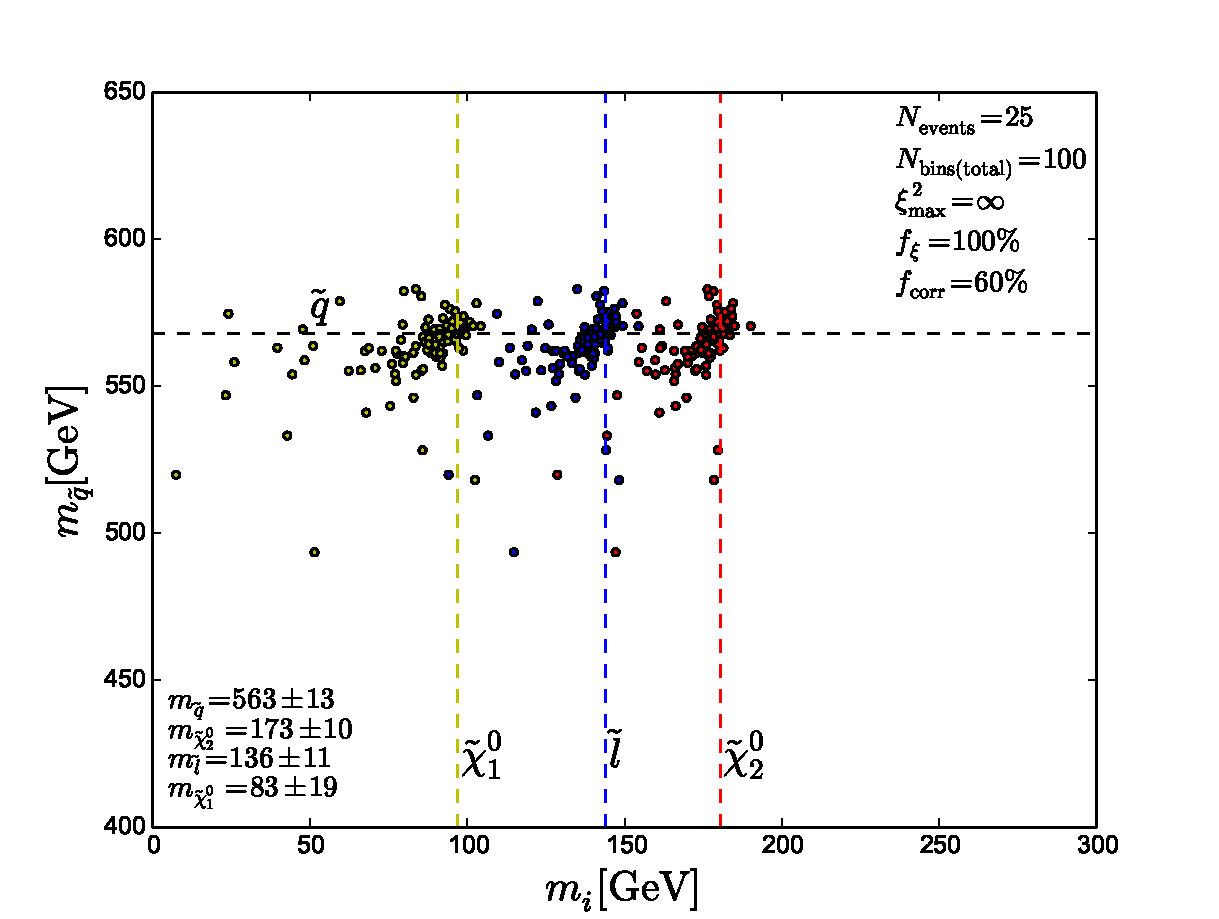
\includegraphics[width=\textwidth]{figures/webber_rec_table/webber_HW-rec_nocut.pdf}
		\caption{ } 
		\label{fig:webber_rec_scatter_tolerance-comparison_b}
	\end{subfigure}
	\caption{Reproduction of Webber's results (corresponding to figure \ref{fig:webber_scatter} and the first row of table \ref{table:webber_original}) for (a) original convergence tolerance and (b) a lower tolerance criterion.}
	\label{fig:webber_rec_scatter_tolerance-comparison}
\end{figure}
Our reproduction of fig.\ \ref{fig:webber_scatter} is shown in fig.\ \ref{fig:webber_rec_scatter_tolerance-comparison_a}, and our reproduction of table \ref{table:webber_original} is given in table \ref{table:webber_softsusy}.
\begin{table}[hbt]
	\centering
	\begin{tabular}{| l | l | l | l  || l | l | l | l |}
		\hline
		$\delta p/p$ & $\xi^2_\mathrm{max}$ & $f_\xi$ & $f_\mathrm{cor}$ & $m_{\tilde q} (540)$ & $m_{\tilde \chi_2^0} (177)$ & $m_{\tilde l} (143)$ & $m_{\tilde \chi_1^0} (96)$ \\
		\hline \hline
		0 & 	$\infty$ &	100 \%	& 65 \%	& $566 \pm 9$	&	$180 \pm 2$		&	$144 \pm 2$	& 	$97 \pm 3$	\\
		0 &		100 &		85 \%	& 67 \% & $567 \pm 6$	&	$180 \pm 1$		&	$144 \pm 1$	&	$97 \pm 3$	\\
		5 \% &	$\infty$ &	100 \%	& 43 \% & $564 \pm 26$	& 	$181 \pm 14$	&	$145 \pm 10$&	$94 \pm 15$ \\
		5 \% &	100 &		52 \%	& 48 \% & $566 \pm 10$	&	$180 \pm 2$		& 	$145 \pm 2$	&	$96 \pm 4$	\\
		10 \% &	$\infty$ &	100 \%	& 33 \% & $551 \pm 33$	&	$180 \pm 15$	&	$144 \pm 11$&	$91 \pm 24$	\\
		10 \% &	200 &		43 \%	& 36 \% & $559 \pm 17$	& 	$177 \pm 11$	&	$143 \pm 11$&	$91 \pm 20$ \\
		\hline
	\end{tabular}
	\caption{Our reproduction of table \ref{table:webber_original}, using Webber's code \cite{Webber:epost} with original settings, except with the masses from SoftSUSY.}
	\label{table:webber_softsusy}
\end{table}







However, the tolerance setting in {Minuit} can be adjusted. When we rerun the code used to produce fig.\ \ref{fig:webber_rec_scatter_tolerance-comparison_a} with the tolerance set to $10^{-12}$, we get the fit shown in \ref{fig:webber_rec_scatter_tolerance-comparison_b}. The results are not dramatically altered, but there are some features to notice: There is a clear tendency to a linear correlation between the masses. This is a feature we should expect physically: If one reduces one of the masses, {\it e.g.}\ the squark, then this should affect the fit of the other masses, reducing them correspondingly.\footnote{This is part of the reason why these kinds of mass reconstruction methods very often reconstruct the squared mass {\it difference} rather than the masses themselves.} The fact that this physically reasonable degenerate direction appears when the tolerance is reduced indicates that a such a reduction is necessary to achieve reliable results. We also note that the fitted masses now seem slightly biased toward lower values. Finally we note that while the mean value and errors are still consistent with the true values, their accuracy is somewhat reduced. Particularly so for the LSP, where the fit is reduced from $99 \pm 3$ GeV to $83 \pm 19$ GeV, compared to the true value of 97 GeV.

These fit results, with the low tolerance setting, are still not bad. However, in table \ref{table:webber_original}, Webber also gives best-fit values where he has applied smearing to the four-momenta, as a crude approximation to the effects of limited detector resolution. The momentum smearing is done by smearing the spatial components according to a gaussian distribution of a given r.m.s. width $\delta p/p$, and then defining the energy in such a way that the invariant mass is unchanged \cite{Webber:epost}.
\begin{figure}[hbt]
	\centering
	\begin{subfigure}[b]{0.6\textwidth}
		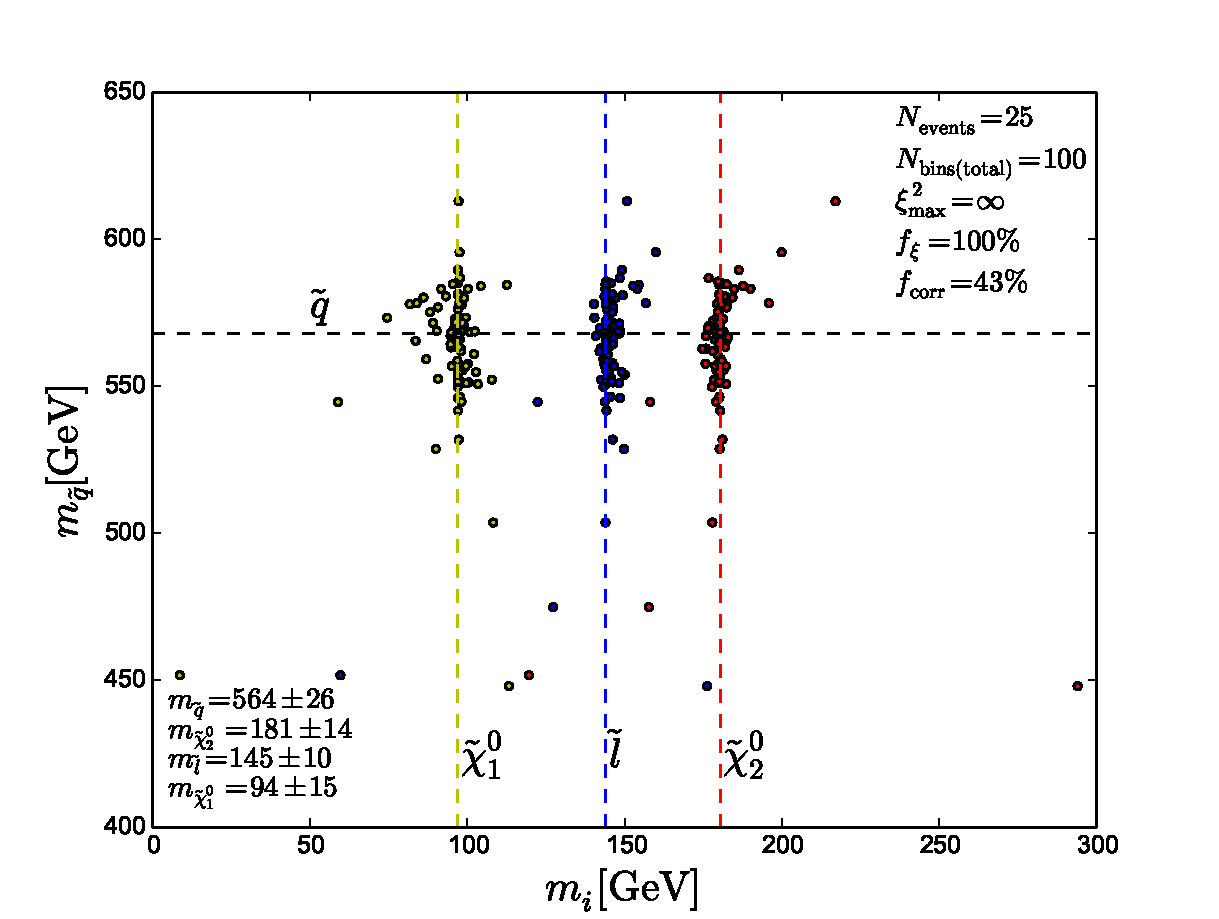
\includegraphics[width=\textwidth]{figures/webber_rec_table/webber_HW-rec_OFL_minuit-minimizer_hightol_5pmomsmear_nocut.pdf} 
		\caption{ }
	\end{subfigure}

	\begin{subfigure}[b]{0.6\textwidth}
		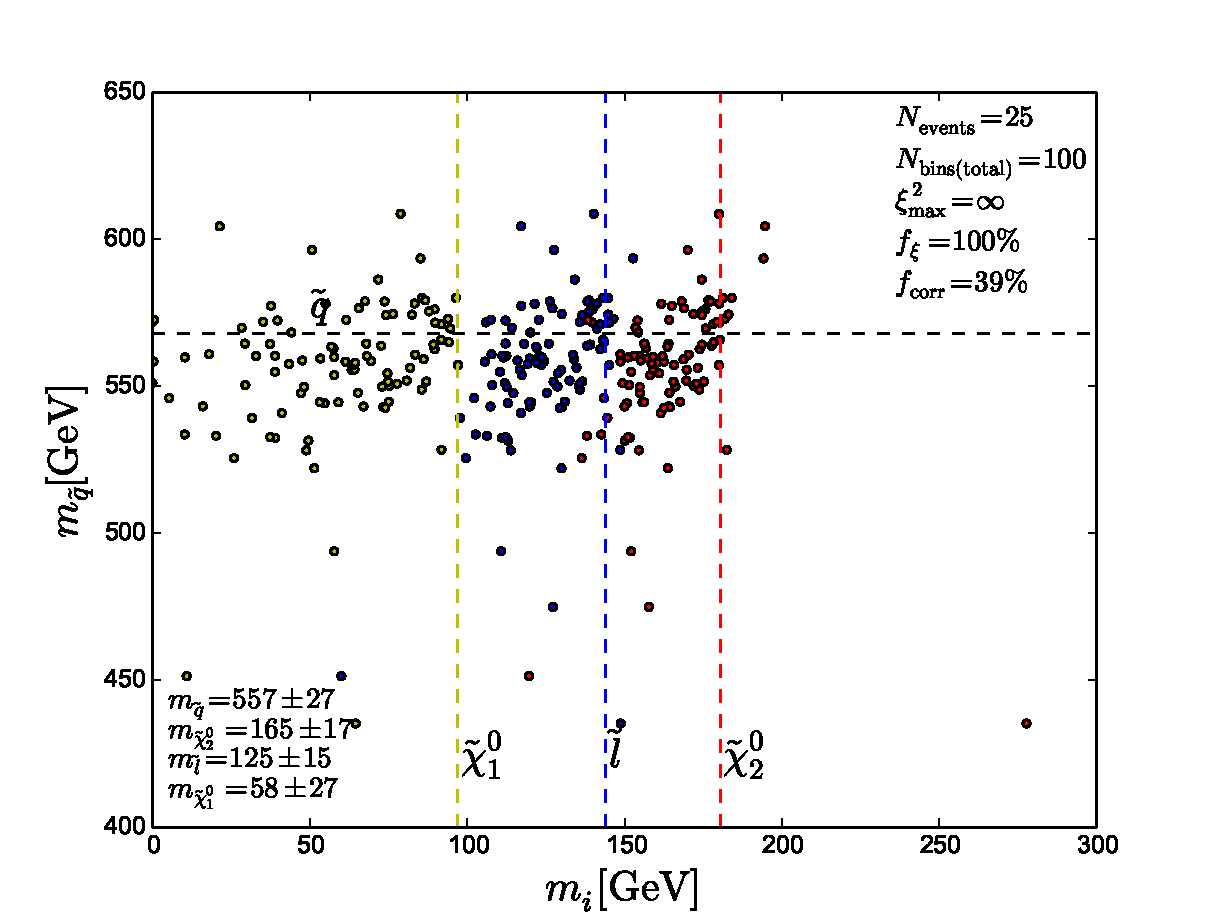
\includegraphics[width=\textwidth]{figures/webber_rec_table/webber_HW-rec_OFL_minuit-minimizer_lowtol_5pmomsmear_nocut.pdf}
		\caption{ } 
	\end{subfigure}
	\caption{Reproduction of Webber's 5\% momentum-smeared fit (corresponding to the third row of table \ref{table:webber_original}) for (a) original convergence tolerance and (b) a lower tolerance criterion.}
	\label{fig:webber_rec_scatter_tolerance-comparison_5pmomsmear}
\end{figure} 
In fig.\ \ref{fig:webber_rec_scatter_tolerance-comparison_5pmomsmear} we show scatter plots of the fits to the dataset smeared with $\delta p/p = 5 \%$, minimized with original and reduced tolerance, again using Webber's code for event generation and minimization. The fit with original tolerance is consistent with fig.\ 3 of \cite{Webber:2009vm}, as it should be. However, when the tolerance is reduced, the fit results are worsened considerably. Since each event is smeared individually, this appears to greatly affect the position of the minimum. Again we see that the LSP (yellow) recieves the roughest treatment, being pushed to much lower values than the true one in most cases. The results are even worse for the 10 \% smeared dataset. We also note that in the HERWIG code Webber uses, initial-state radiation of photons in SUSY decays is switched off, which may contribute to making the measurement unrealistically good.\marginpar{Are doesn't think this is a big effect, but I am not sure. I did complete momentum conservation in my events same as Webber, in practice turning off ISR. Should consider checking, or rewriting.}




% \begin{figure}[hbt]
% 	\centering
% 	\begin{subfigure}[b]{0.6\textwidth}
% 		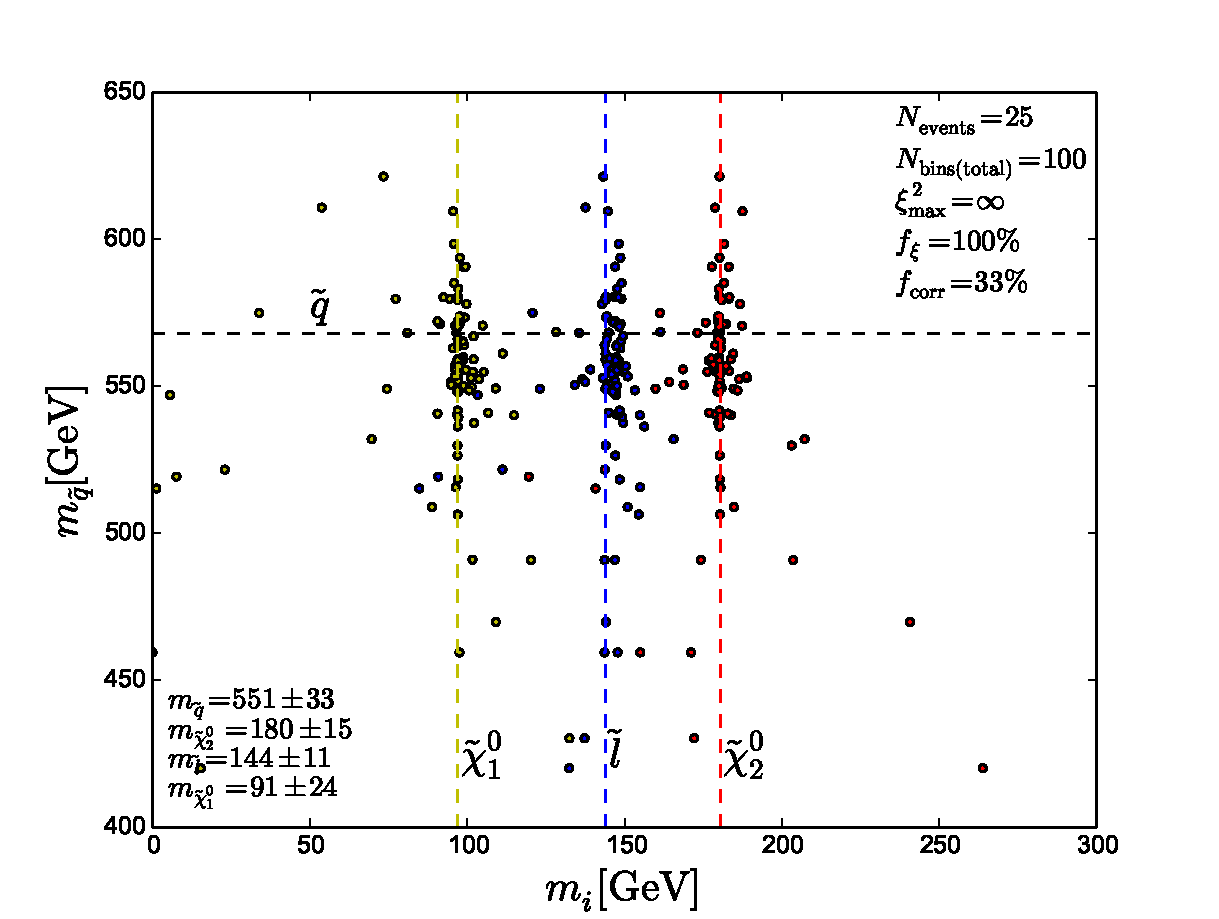
\includegraphics[width=\textwidth]{figures/webber_rec_table/webber_HW-rec_OFL_minuit-minimizer_hightol_10pmomsmear_nocut.pdf} 
% 		\caption{ }
% 	\end{subfigure}

% 	\begin{subfigure}[b]{0.6\textwidth}
% 		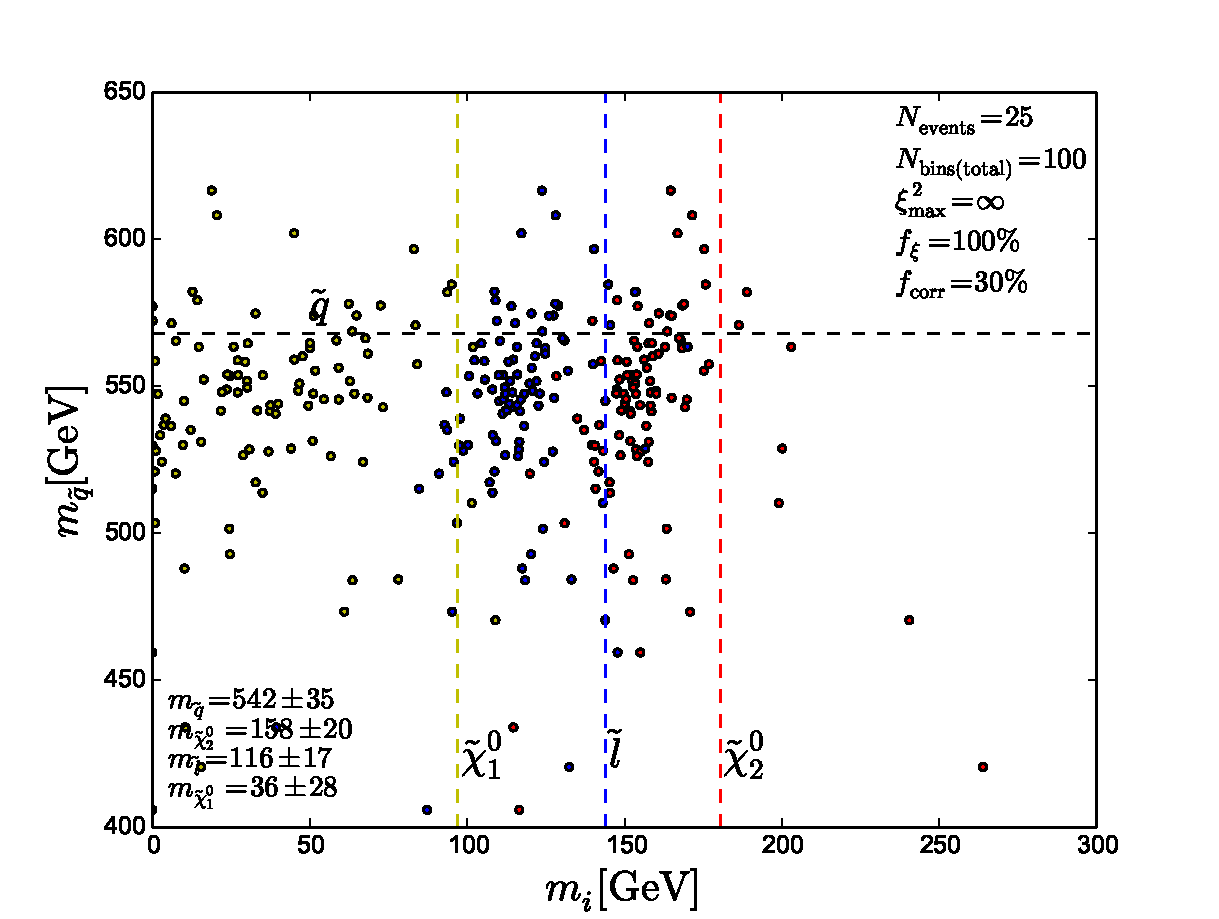
\includegraphics[width=\textwidth]{figures/webber_rec_table/webber_HW-rec_OFL_minuit-minimizer_lowtol_10pmomsmear_nocut.pdf}
% 		\caption{ } 
% 	\end{subfigure}
% 	\caption{Reproduction of Webber's 10 \% momentum-smeared fit (corresponding to figure 3 of \cite{Webber:2009vm} and the fifth row of table \ref{table:webber_original}) for (a) original convergence tolerance and (b) a lower tolerance criterion.}
% 	\label{fig:webber_rec_scatter_tolerance-comparison_10pmomsmear}
% \end{figure}

However, Webber also investigates the effects of imposing a {\it cut} on the $\xi^2$ value obtained at the minimum. In his fits, this cut tends to remove the bad events, giving a better fit. Applying a cut also helps for the reduced-tolerance fit, although it does not recover Webber's original low error estimate. In table \ref{table:webber_rec_lowtol} we reproduce table \ref{table:webber_original} for the reduced-tolerance fit. We note that the fraction of samples passing the $\xi^2$ cut is drastically reduced compared to table \ref{table:webber_original}. The fraction of events where the best-fit combination is the true one is also reduced by about half. 

\begin{table}[hbt]
	\centering
	\begin{tabular}{| l | l | l | l  || l | l | l | l |}
		\hline
		$\delta p/p$ & $\xi^2_\mathrm{max}$ & $f_\xi$ & $f_\mathrm{cor}$ & $m_{\tilde q} (568)$ & $m_{\tilde \chi_2^0} (180)$ & $m_{\tilde l} (144)$ & $m_{\tilde \chi_1^0} (97)$ \\
		\hline \hline
		0 & 	$\infty$ &	100 \%	& 36 \%	& $563 \pm 13$	&	$173 \pm 10$	&	$136 \pm 11$	& 	$83 \pm 19$	\\
		0 &		100 &		35 \%	& 52 \% & $565 \pm 9$	&	$175 \pm 8$		&	$138 \pm 9$	&	$86 \pm 16$	\\
		5 \% &	$\infty$ &	100 \%	& 31 \% & $557 \pm 27$	& 	$165 \pm 17$	&	$125 \pm 15$&	$58 \pm 27$ \\
		5 \% &	100 &		13 \%	& 43 \% & $558 \pm 14$	&	$164 \pm 11$	& 	$126 \pm 12$	&	$65 \pm 22$	\\
		10 \% &	$\infty$ &	100 \%	& 29 \% & $542 \pm 35$	&	$158 \pm 20$	&	$116 \pm 17$&	$36 \pm 28$	\\
		10 \% &	200 &		15 \%	& 33 \% & $549 \pm 20$	& 	$155 \pm 12$	&	$116 \pm 12$&	$38 \pm 25$ \\
		\hline
	\end{tabular}
	\caption{Reproduction of the fits in table \ref{table:webber_softsusy}, but with reduced convergence tolerance.}
	\label{table:webber_rec_lowtol}
\end{table}

\section{The starting-point dependence of the best-fit point}
\label{sec:SP-dependence_webber}

There is also another potential issue with Webber's analysis. It has to do with the fact that the best-fit search is started at the true mass values.  In a real experiment, these parameters are exactly the unknowns we wish to find. Starting the search here is in principle fine as long as we are sure that the algorithm always finds the true global minimum. So we must investigate what happens if we start our search in some other point. We have done this, and discover that this greatly affects the location of the best-fit points.
\begin{figure}[hbt]
	\centering
	\begin{subfigure}[b]{0.45\textwidth}
		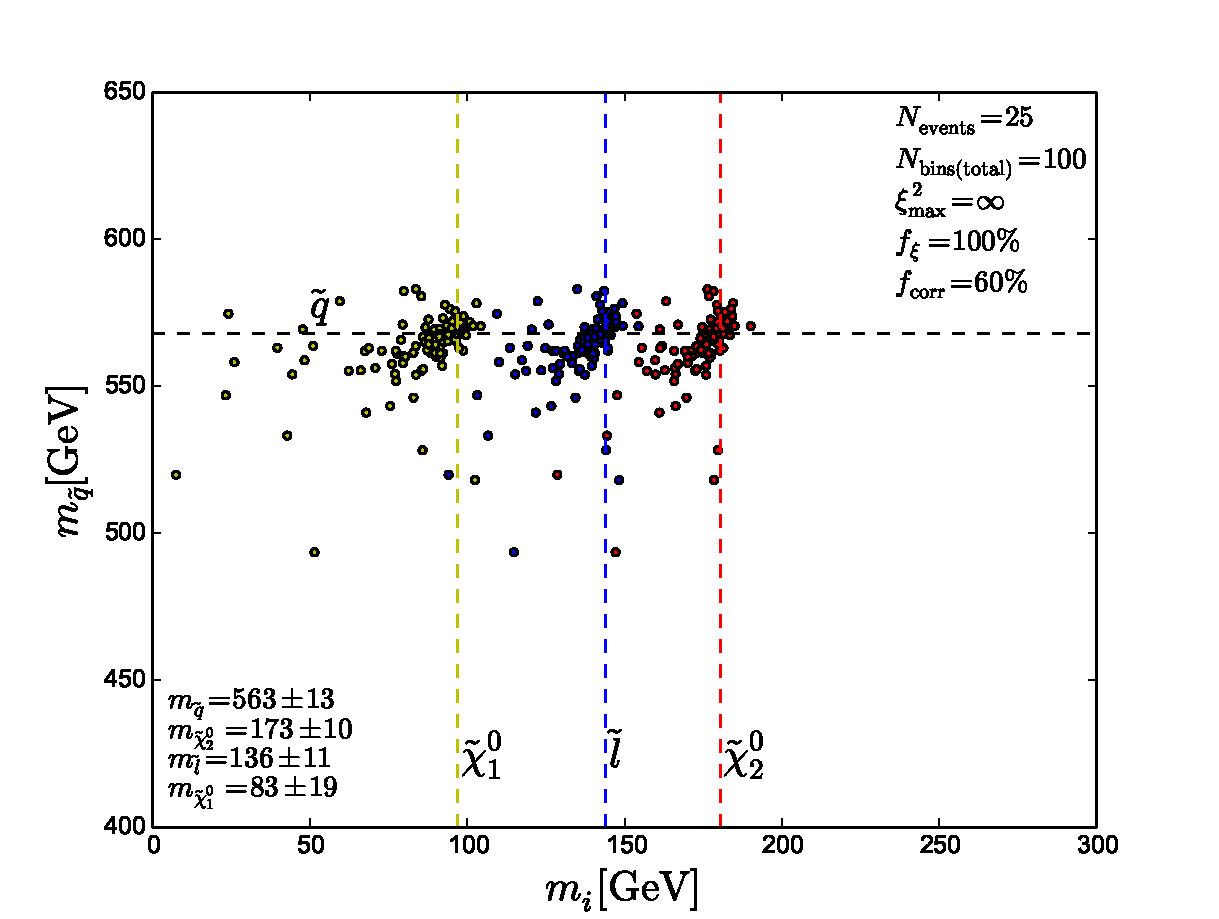
\includegraphics[width=\textwidth]{figures/webber_rec_table/webber_HW-rec_nocut.pdf} 
		\caption{ }
	\end{subfigure}
	\begin{subfigure}[b]{0.45\textwidth}
		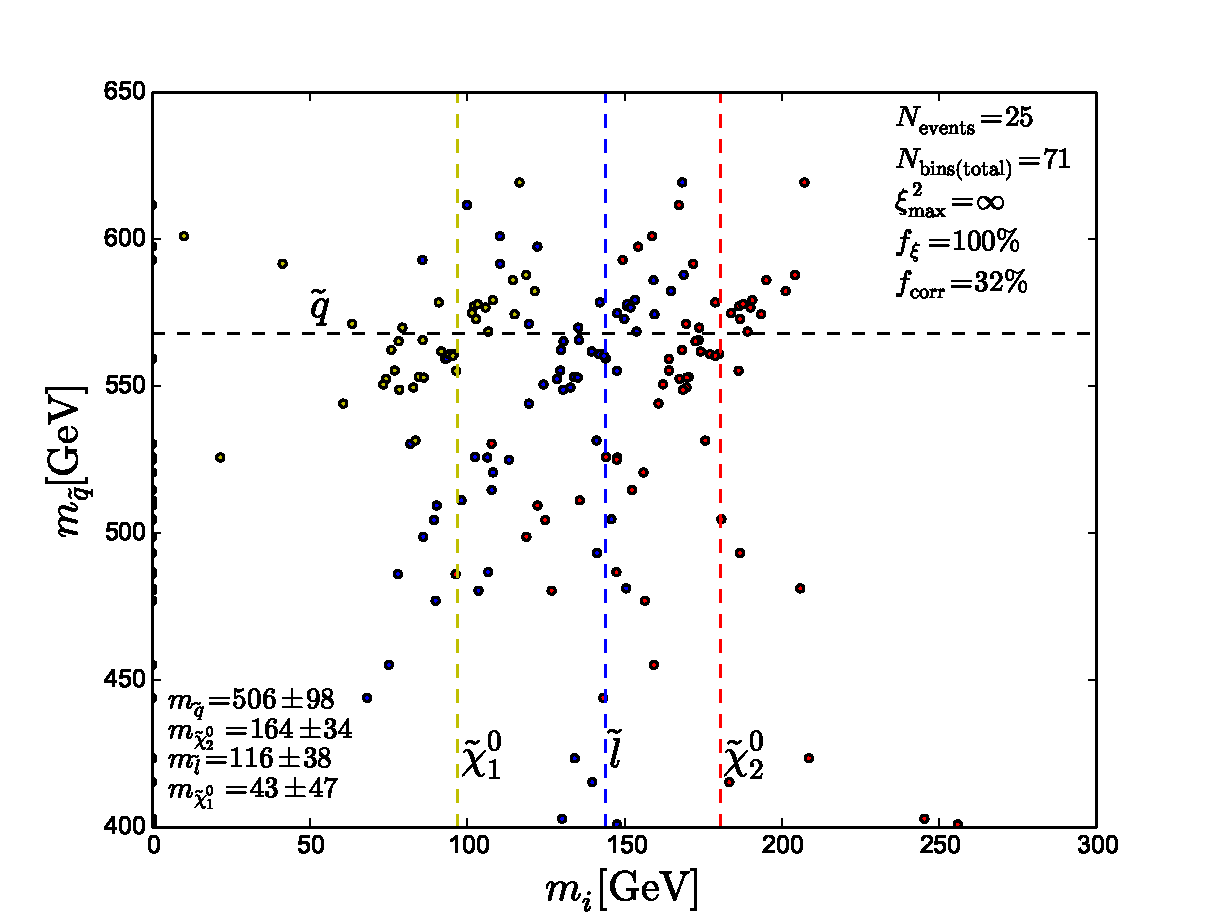
\includegraphics[width=\textwidth]{figures/webber_rec_table/webber-rec_wrong_starting_point-400-300-200-100_lowtol.pdf}
		\caption{ } 
	\end{subfigure}

	\begin{subfigure}[b]{0.45\textwidth}
		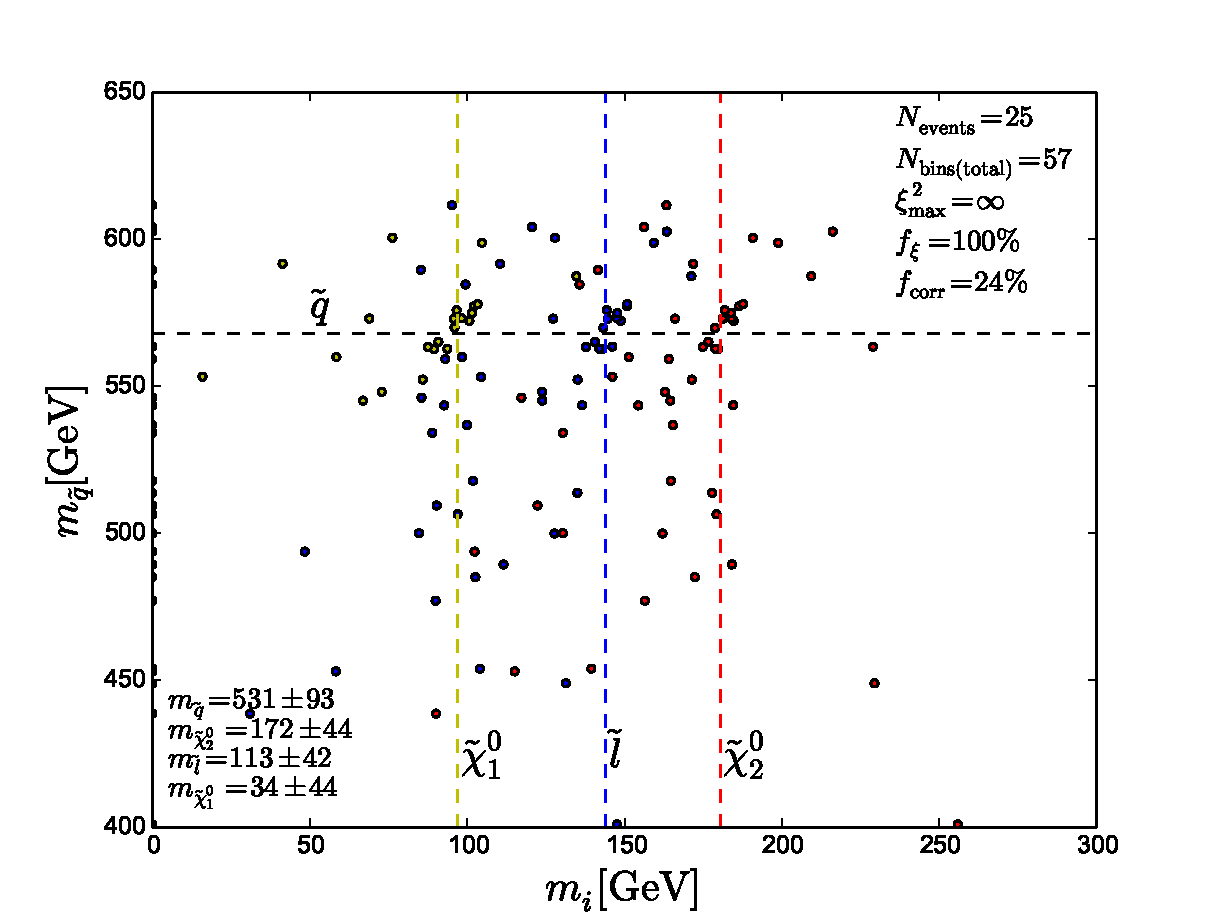
\includegraphics[width=\textwidth]{figures/webber_rec_table/webber-rec_wrong_starting_point-800-500-300-50_lowtol.pdf} 
		\caption{ }
	\end{subfigure}
	\begin{subfigure}[b]{0.45\textwidth}
		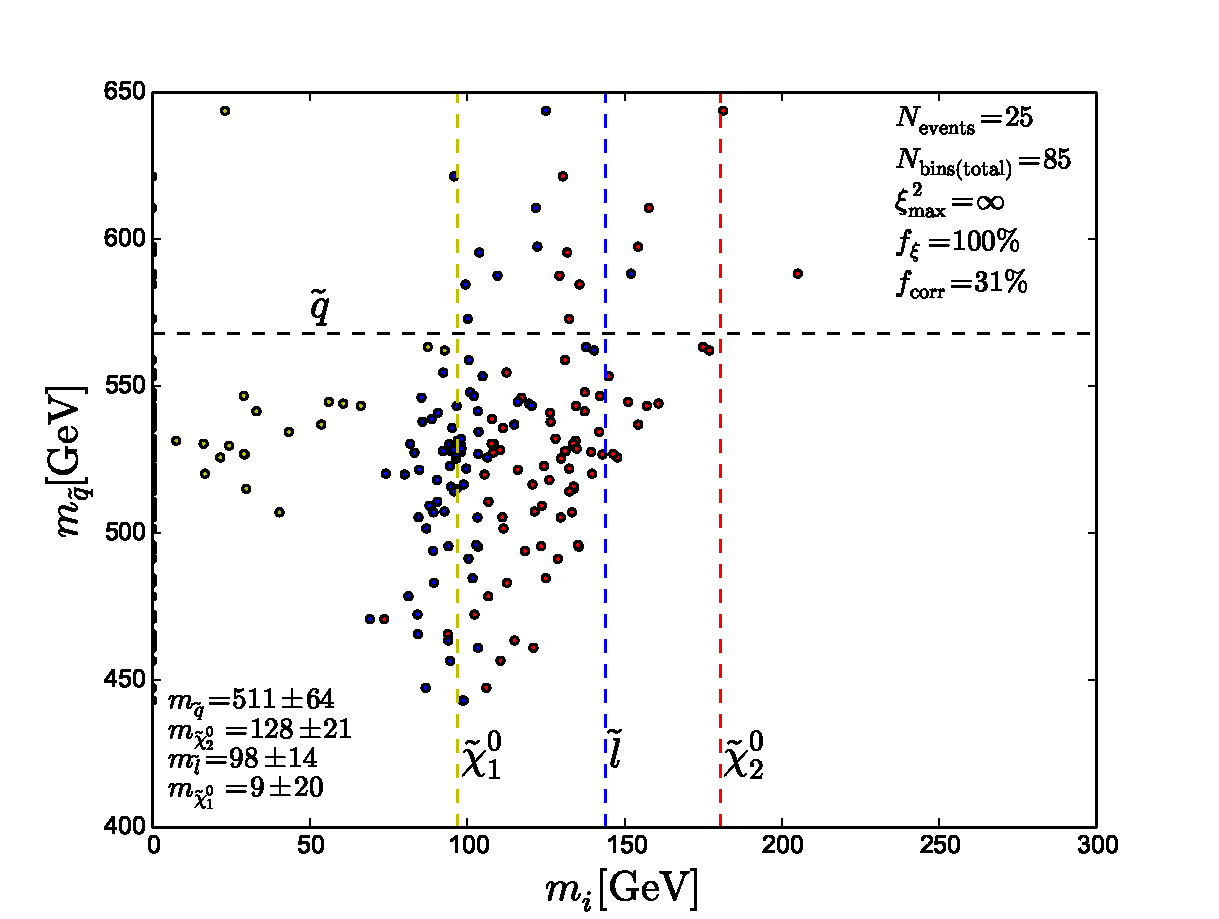
\includegraphics[width=\textwidth]{figures/webber_rec_table/webber-rec_wrong_starting_point-1000-100-80-30_lowtol.pdf}
		\caption{ } 
	\end{subfigure}
	\caption{Minimization on the unsmeared {\tt HERWIG} dataset for different starting points: $\vec M = (568, 180, 144, 97)$ (the TMP) in {\bf (a)}, $\vec M = (400, 300, 200, 100)$  in {\bf (b)}, $\vec M = (800, 500, 300, 50)$ in {\bf (c)} and $\vec M = (1000, 100, 80, 30)$ in {\bf (d)}.}
	\label{fig:starting_point_sensitivity_combinatorics}
\end{figure}
In fig.\ \ref{fig:starting_point_sensitivity_combinatorics} we show the best-fit points for four low-tolerance minimizations on the {\tt HERWIG} dataset. Subfig.\ (a) is the same as \ref{fig:webber_rec_scatter_tolerance-comparison} (b), the minimization started from the true mass point (TMP). The other three are minimizations from other starting points, selected to illustrate other plausible mass spectra: one where both the masses and the mass differences are smaller (b); one where they are larger (c); and one where there is a large splitting between a heavy squark and three very light masses (d). It is obvious that the fit -- the location of the best-fit point, and also the number of samples where convergence is obtained, indicated by the number $N_\mathrm{bins}$ in each plot -- is hugely dependent on where we start the search. For instance, the mean value and standard errors of the squark masses for the samples range from $506 \pm 98 \mathrm{GeV}$ to $563 \pm 13 \mathrm{GeV}$. We also note that in the latter case, which is the minimization from the TMP, the mean values from the other three starting points fall outside the margin of error.\marginpar{Did I manage to get this sentence to make sense?}



It might, however, be that the function has multiple local minima, giving rise to the behaviour in fig.\ \ref{fig:starting_point_sensitivity_combinatorics}, but that the {\it global} minimum is the one we find by starting in the TMP. To investigate this, we have run minimizations (with low tolerance) where we perturb the starting point of each of the four parameters for each event sample away from the TMP by a gaussian distribution of width 10 or 20 GeV. This is a minor perturbation relative to the masses. The minimization results are shown in table \ref{table:webber_rec_lowtol_perturbedSP} for perturbations of 10 (top) and 20 (bottom) GeV. The standard errors of the fit increase considerably compared with \ref{table:webber_rec_lowtol}. \marginpar{Smear with 10 \% and 20 \% of the masses too?}
 
% we have made a scan of many starting points, minimizing the whole 100 bin dataset from each starting point. We selected five different values for each of the four SUSY masses and checked all combinations which make physical sense ({\it i.e.\ }where the mass hierarchy is present). This gave a total of 132 different starting points, which were indexed from 1 to 132. The TMP was point number 34. For each bin we then checked which index had the lowest $\xi^2$ value. Figure \ref{fig:webber_rec_hist_starting_points} shows a histogram of this. We see that number 34, the TMP, indeed dominates, but it is only the lowest in 14 of the 100 bins. The other 86 bins are distributed quite evenly among the other starting points. This leads us to conclude that the minimization, using this technique, simply is not well defined: There is no reasonable hope that we will be able to find a reliable best-fit estimate in an experimental situation where the TMP is unknown. This is especially true given that this scan was done on the unsmeared dataset -- we should expect even worse results when the resolution gets blurred by uncertainties.

% \begin{figure}[hbt]
% 	\centering
% 	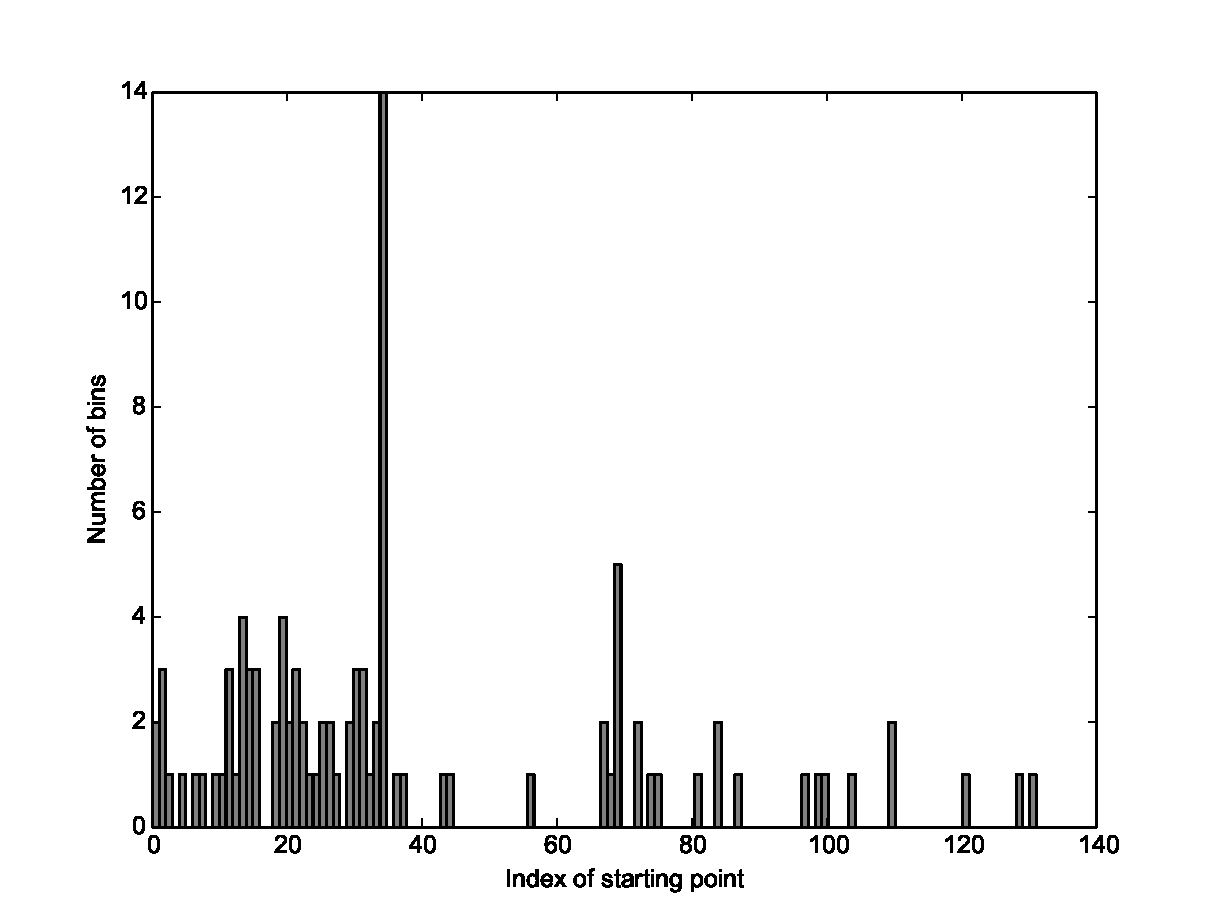
\includegraphics[width=0.8\textwidth]{figures/webber_rec_table/histogram_of_starting_points_with_lowest_minimal_value.pdf}
% 	\caption{A histogram of 100 data bins minimized from different starting points, showing distribution of lowest $\xi^2$ values. See the text for details.}
% 	\label{fig:webber_rec_hist_starting_points}
% \end{figure}


\begin{table}[hbt]
	\centering
	\begin{tabular}{| l | l | l | l  || l | l | l | l |}
		\hline
		$\delta p/p$ & $\xi^2_\mathrm{max}$ & $f_\xi$ & $f_\mathrm{cor}$ & $m_{\tilde q} (568)$ & $m_{\tilde \chi_2^0} (180)$ & $m_{\tilde l} (144)$ & $m_{\tilde \chi_1^0} (97)$ \\
		\hline \hline
		10 GeV: & & & & & & & \\ 
		\hline
		0 & 	$\infty$ &	100 \%	& 47 \%	& $559 \pm 29$	&	$170 \pm 19$	&	$131 \pm 20$	& 	$68 \pm 38$	\\
		0 &		100 &		76 \%	& 48 \% & $564 \pm 12$	&	$175 \pm 13$		&	$137 \pm 14$	&	$83 \pm 25$	\\
		5 \% &	$\infty$ &	100 \%	& 38 \% & $557 \pm 24$	& 	$163 \pm 18$	&	$123 \pm 20$&	$52 \pm 36$ \\
		5 \% &	100 &		55 \%	& 37 \% & $559 \pm 16$	&	$168 \pm 13$	& 	$130 \pm 15$	&	$72 \pm 22$	\\
		10 \% &	$\infty$ &	100 \%	& 28 \% & $542 \pm 42$	&	$153 \pm 19$	&	$113 \pm 21$&	$19 \pm 31$	\\
		10 \% &	200 &		44 \%	& 26 \% & $550 \pm 21$	& 	$159 \pm 18$	&	$119 \pm 20$&	$38 \pm 36$ \\
		\hline
		20 GeV: & & & & & & & \\ 
		\hline
		0 & 	$\infty$ &	100 \%	& 42 \%	& $555 \pm 32$	&	$167 \pm 23$	&	$126 \pm 24$	& 	$60 \pm 41$	\\
		0 &		100 &		67 \%	& 44 \% & $564 \pm 14$	&	$173 \pm 14$	&	$135 \pm 16$	&	$82 \pm 24$	\\
		5 \% &	$\infty$ &	100 \%	& 34 \% & $550 \pm 45$	& 	$162 \pm 23$	&	$123 \pm 22$&	$46 \pm 39$ \\
		5 \% &	100 &		54 \%	& 34 \% & $554 \pm 23$	&	$163 \pm 21$	& 	$125 \pm 21$	&	$63 \pm 31$	\\
		10 \% &	$\infty$ &	100 \%	& 28 \% & $543 \pm 37$	&	$153 \pm 25$	&	$125 \pm 21$&	$16 \pm 32$	\\
		10 \% &	200 &		37 \%	& 27 \% & $539 \pm 22$	& 	$151 \pm 20$	&	$113 \pm 18$&	$24 \pm 31$ \\
		\hline
	\end{tabular}
	\caption{Reproduction of the fits in table \ref{table:webber_rec_lowtol} with perturbations of 10 and 20 GeV, respectively, on the starting points.}
	\label{table:webber_rec_lowtol_perturbedSP}
\end{table}



\clearpage

\section{Without combinatorics}

If we for a moment forget about the combinatorics, and evaluate only the true particle combination for each event, then the minimization gives consistent results irrespective of starting point. 
\begin{figure}[hbt]
	\centering
	\begin{subfigure}[b]{0.45\textwidth}
		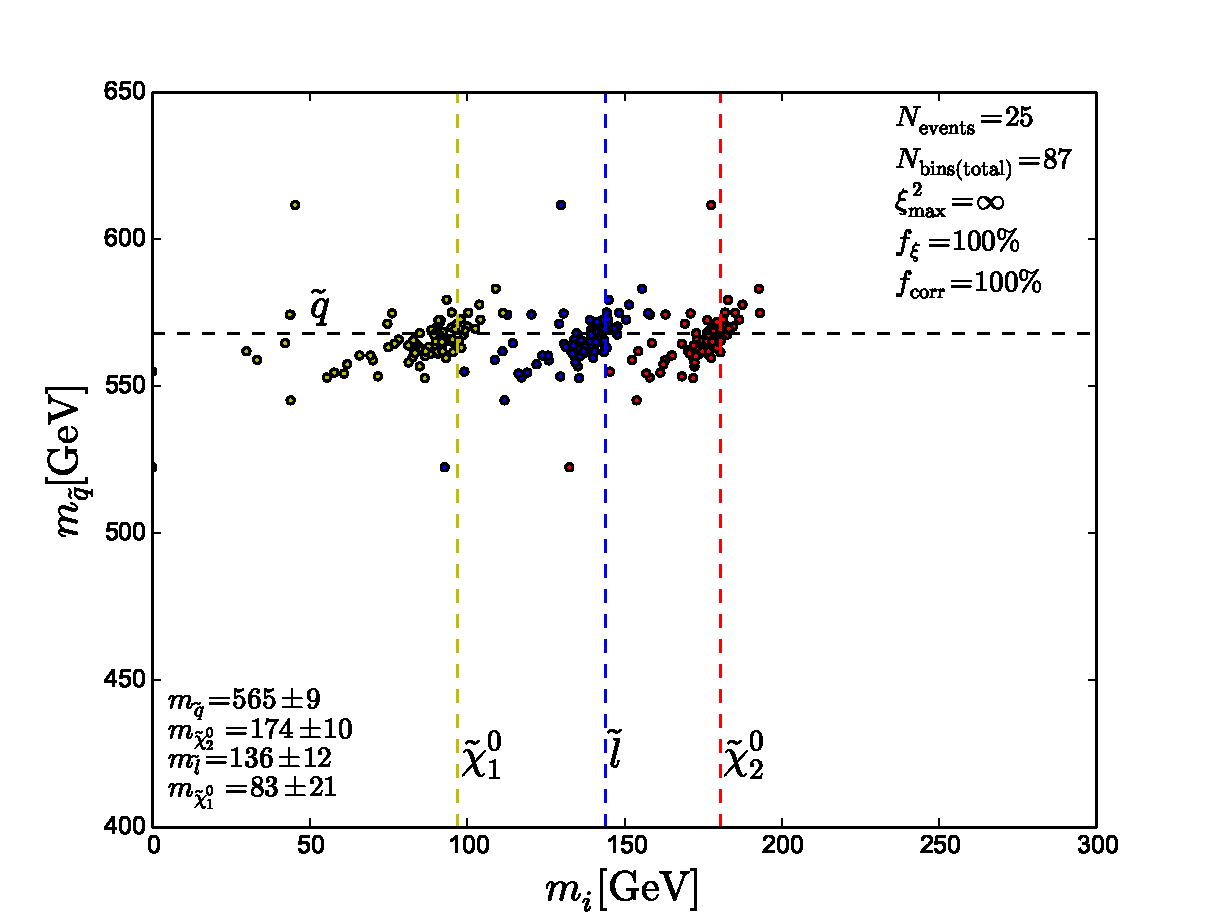
\includegraphics[width=\textwidth]{figures/improving_combinatorics/herwigpp-momcons_nocomb_truemasspoint.pdf} 
		\caption{ }
	\end{subfigure}
	\begin{subfigure}[b]{0.45\textwidth}
		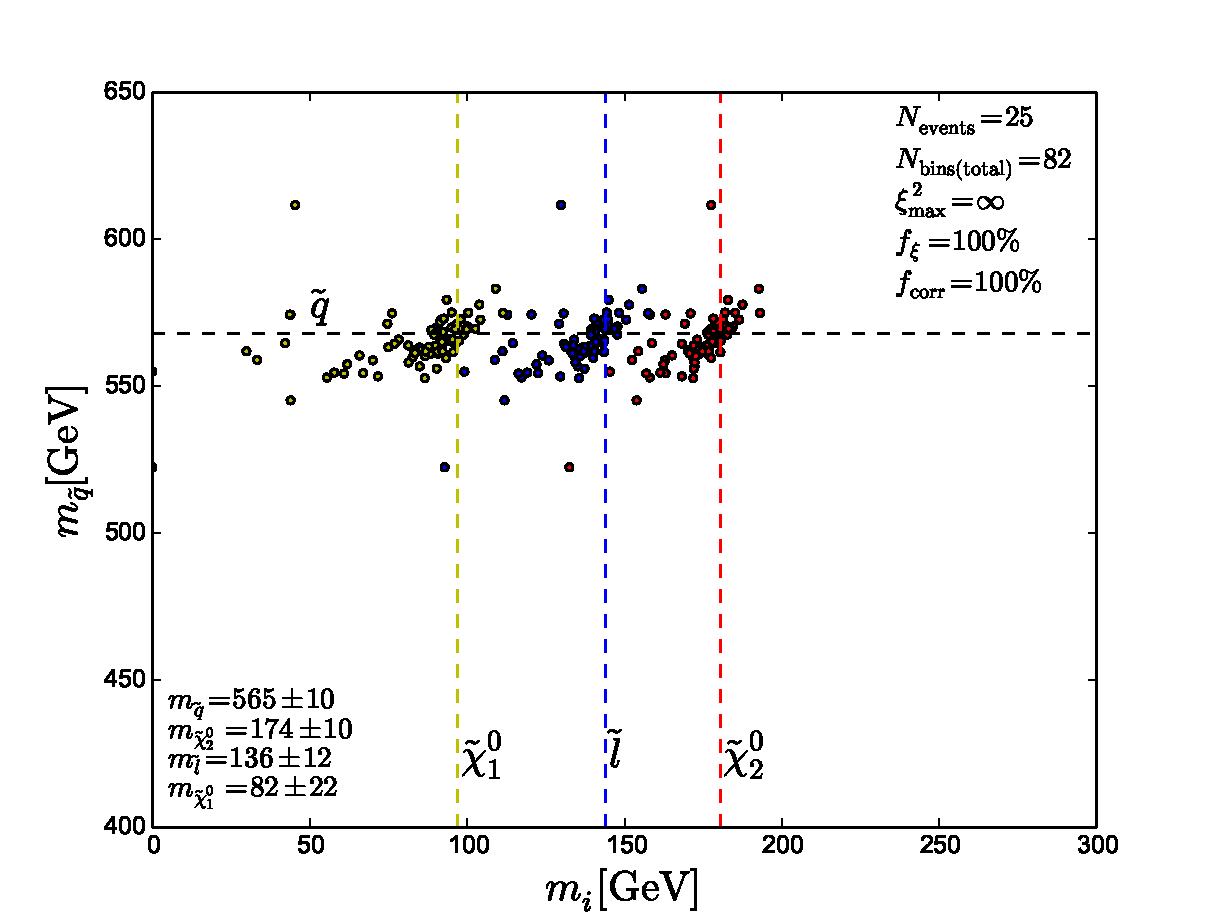
\includegraphics[width=\textwidth]{figures/improving_combinatorics/herwigpp-momcons_nocomb_400-300-200-100.pdf}
		\caption{ } 
	\end{subfigure}

	\begin{subfigure}[b]{0.45\textwidth}
		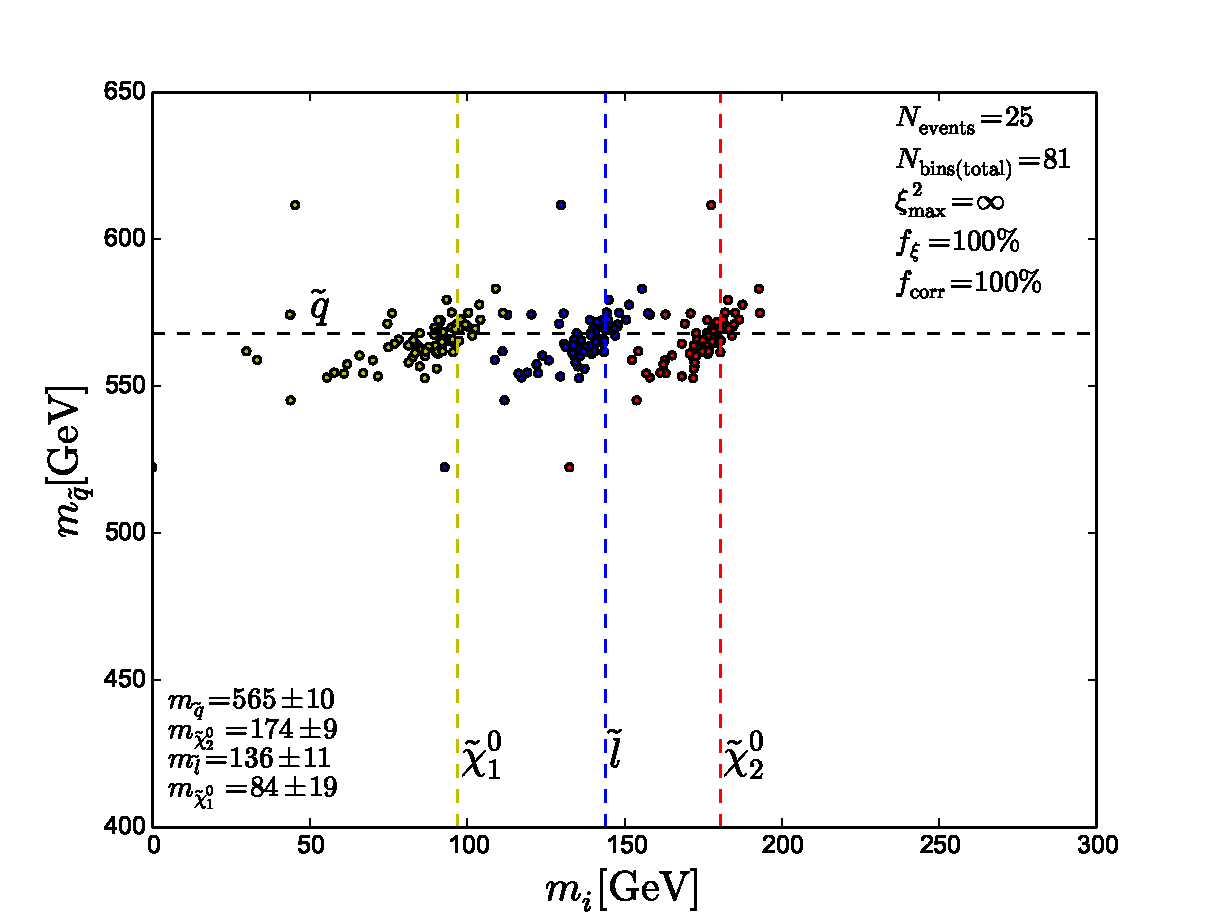
\includegraphics[width=\textwidth]{figures/improving_combinatorics/herwigpp-momcons_nocomb_800-500-300-50.pdf} 
		\caption{ }
	\end{subfigure}
	\begin{subfigure}[b]{0.45\textwidth}
		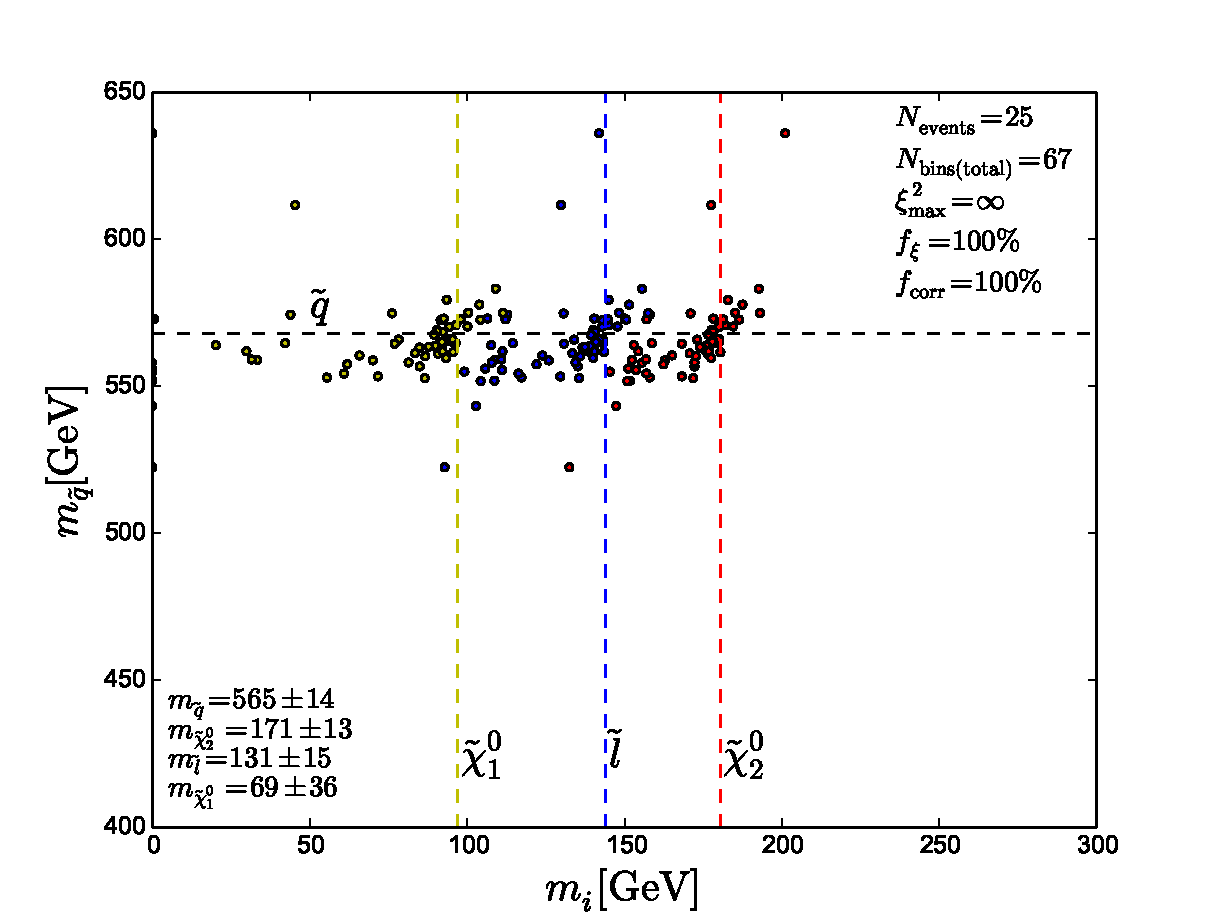
\includegraphics[width=\textwidth]{figures/improving_combinatorics/herwigpp-momcons_nocomb_1000-100-80-30.pdf}
		\caption{ } 
	\end{subfigure}
	\caption{An equivalent fit to figure \ref{fig:starting_point_sensitivity_combinatorics} (on a {\ttfamily Herwig++} dataset), but the $\xi^2$ contribution is only evaluated for the true particle combination in each event.}
	\label{fig:starting_point_sensitivity_no_combinatorics}
\end{figure}
This is illustrated in fig.\ \ref{fig:starting_point_sensitivity_no_combinatorics}, which shows minimization of 100 samples of 25 events minimized with low tolerance, but only evaluated with the correct combination of chain particles.\footnote{This dataset is generated with {\tt Herwig++} version 2.7.1 \cite{Bahr:2008pv} and minimized using our own implementation of the {\tt Simplex} algorithm in C++, included in appendix \ref{ch:simplex}. Only events where the momentum in the chain is exactly conserved -- {\it i.e.}\ no final-state radiation of photons is allowed -- are included. We have checked that this dataset gives identical results with the Fortran {\tt HERWIG} program used in chapter \ref{ch:MC}.} There are differences between the fits, mainly between subfig.\ d and the others. In particular, while about 85 of the samples converge within the set limit of 500 iterations in each of the cases a, b and c (indicated by the value of $N_\mathrm{bins(total)}$ in the top right of each plot), this number is reduced to 67 in subfig.\ d. The starting point in case (d) is characterized by a much larger mass gap between the squark and the $\tilde\chi_2^0$ than in the TMP, which we might surmise would give rise to very different kinematics than we have in our events. In any case, the minimization is not a heavy calculation (the whole minimization of 100 bins, including combinatorics, is done in fractions of a second on a single CPU core), so doing a scan like the one we made above over different starting points is not unrealistic.\marginpar{Is there any point in doing a minimization grid scan here, for the no-combinatorics case? Maybe better to wait until I have handled combinatorics.}

We also keep in mind the effects of momentum smearing, and check the no-combinatorics minimization on the 5 \% smeared dataset for the same four starting points. The plots are shown in fig.\ \ref{fig:moving_on-starting_point_sensitivity_no_combinatorics_5pmomsmear}. We find that it also in this case gives consistent results irrespective of starting point -- but the LSP mass is fitted to zero in most samples.\marginpar{Count number of zero-fits} It appears that when the data is smeared, the method loses its sensitivity to the LSP mass. Or equivalently, we could say that it loses its sensitivity to the absolute mass scale of the problem. This is a well-known problem with methods for mass reconstruction.\marginpar{Might want to cite something if this sentence is kept, or elaborate about mass-squared difference fitting.}
\begin{figure}[hbt]
	\centering
	\begin{subfigure}[b]{0.45\textwidth}
		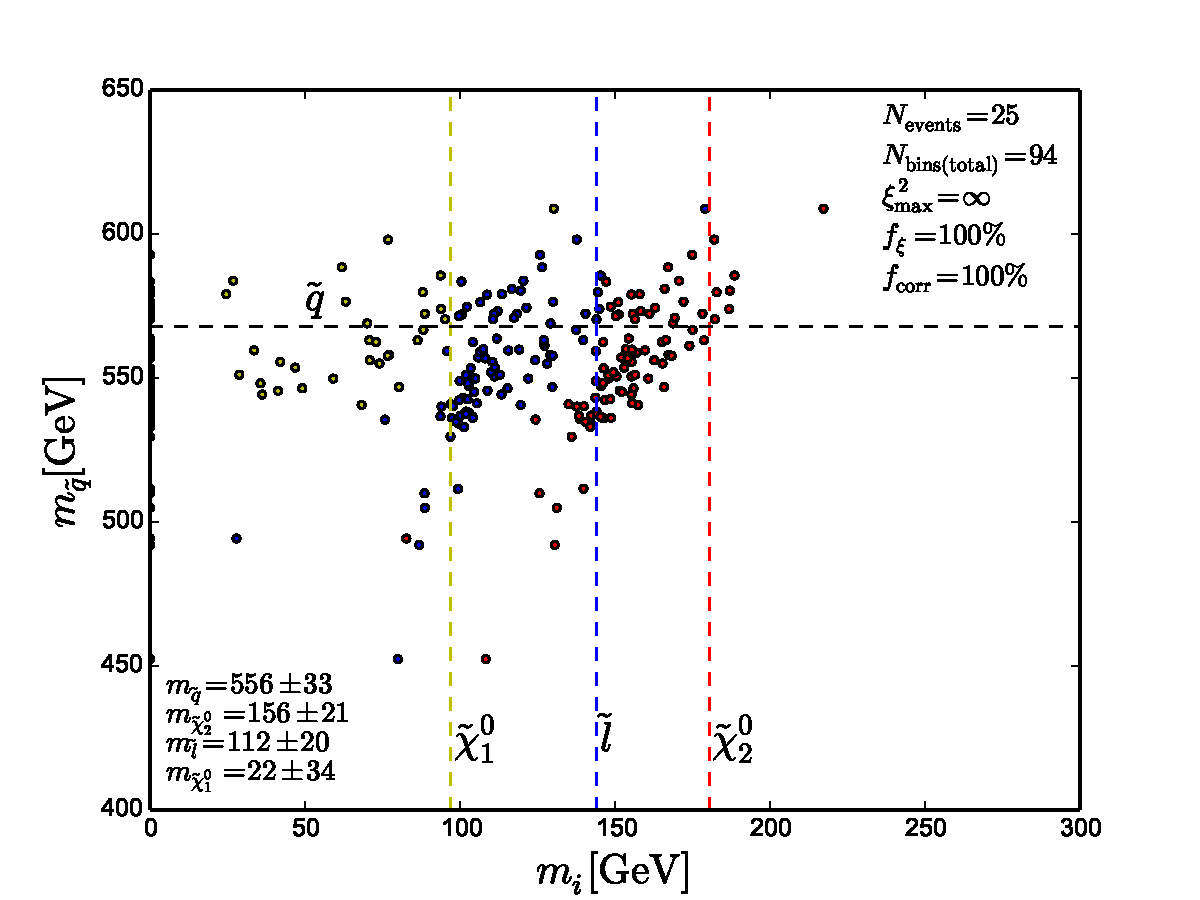
\includegraphics[width=\textwidth]{figures/improving_combinatorics/herwigpp_5psmear_lowtol_nocomb_TMP.pdf} 
		\caption{ }
	\end{subfigure}
	\begin{subfigure}[b]{0.45\textwidth}
		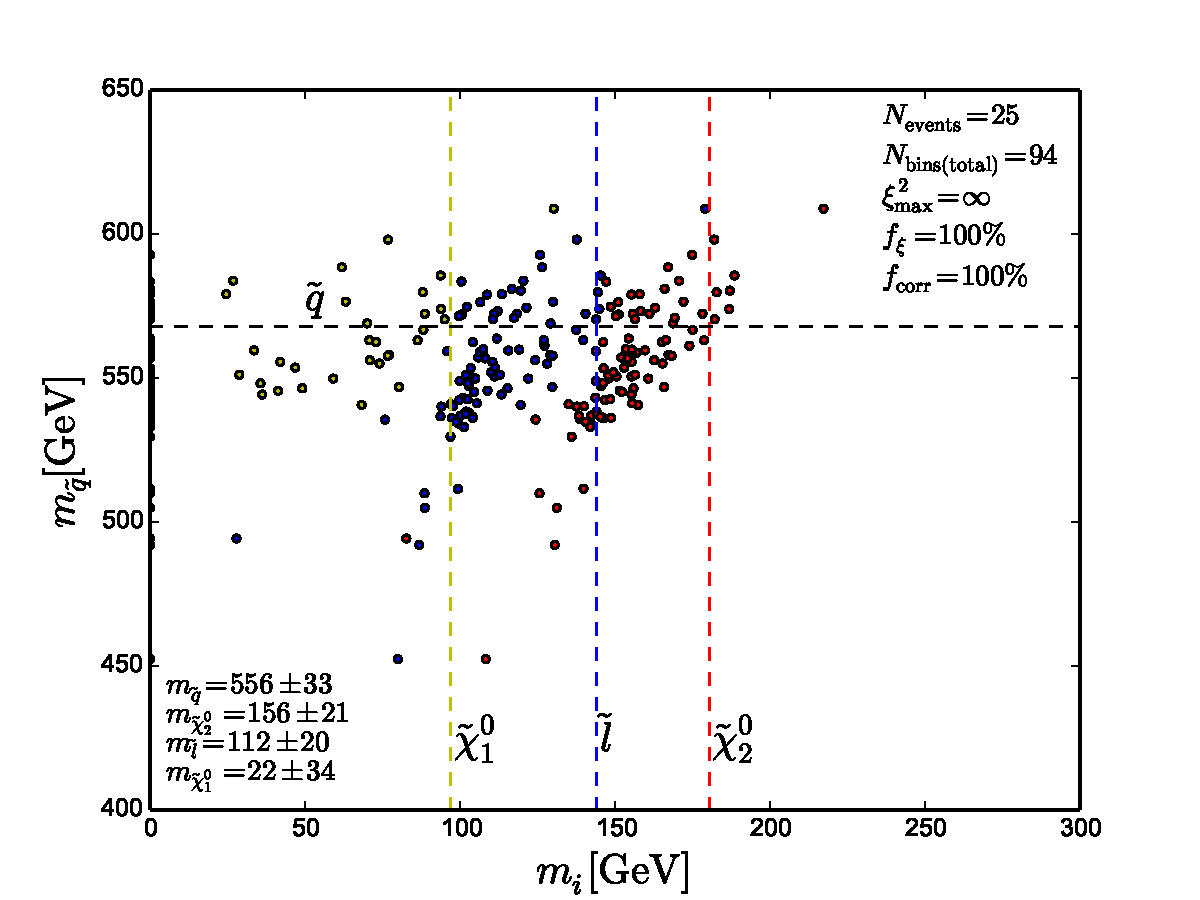
\includegraphics[width=\textwidth]{figures/improving_combinatorics/herwigpp_5psmear_lowtol_nocomb_400-300-200-100.pdf}
		\caption{ } 
	\end{subfigure}

	\begin{subfigure}[b]{0.45\textwidth}
		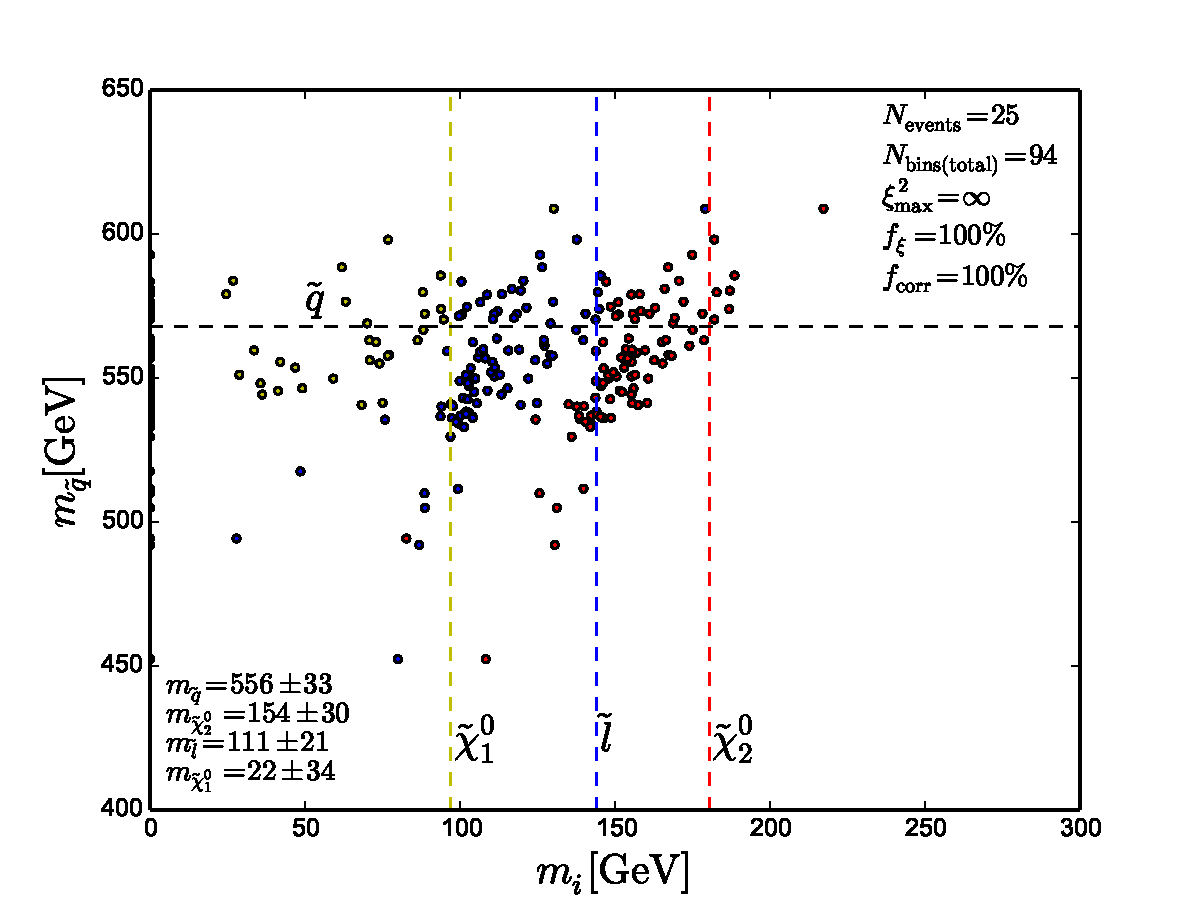
\includegraphics[width=\textwidth]{figures/improving_combinatorics/herwigpp_5psmear_lowtol_nocomb_800-500-300-50.pdf} 
		\caption{ }
	\end{subfigure}
	\begin{subfigure}[b]{0.45\textwidth}
		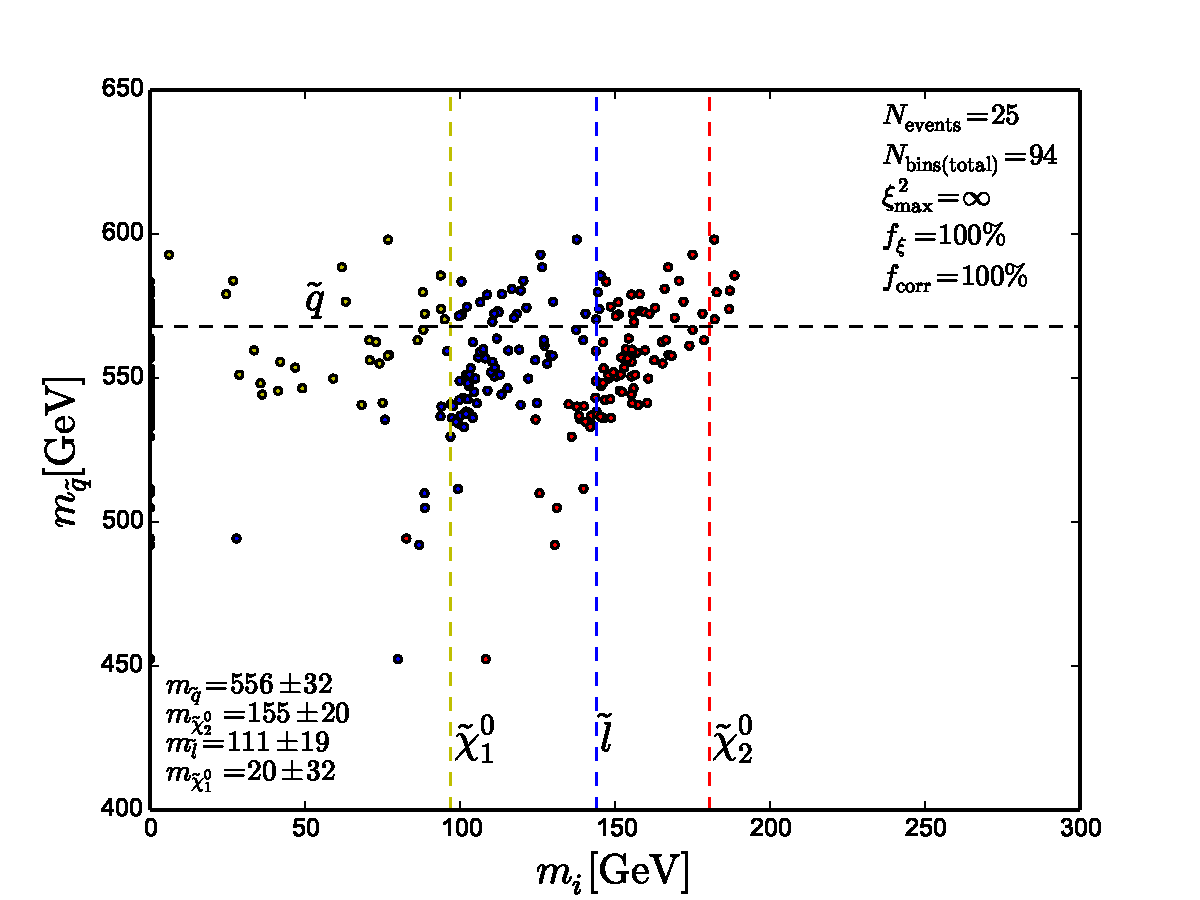
\includegraphics[width=\textwidth]{figures/improving_combinatorics/herwigpp_5psmear_lowtol_nocomb_1000-100-80-30.pdf}
		\caption{ } 
	\end{subfigure}
	\caption{Again the same fit as in \ref{fig:starting_point_sensitivity_combinatorics} and \ref{fig:starting_point_sensitivity_no_combinatorics}, here with a 5 \% smeared dataset and no combinatorics.}
	\label{fig:moving_on-starting_point_sensitivity_no_combinatorics_5pmomsmear}
\end{figure} 






























%%%%%%%%%%%%%%%%%%%%%%%%%%%%%%%%%%%%%%%%%%%%%%%
\chapter{Investigating improvements}%%%%%%%%%%%
%%%%%%%%%%%%%%%%%%%%%%%%%%%%%%%%%%%%%%%%%%%%%%%
With the potentially significant errors inherent in Webber's original suggestion, we will now turn to investigate improvements.


\section{Fitting mass squared differences}
We saw in the previous chapter that, even without taking combinatorical ambiguities into account, the method is insensitive to the absolute mass scale of the decay in many of the samples when the momentum resolution is smeared. In a later article \cite{Nojiri:2010dk}, Webber {\it et al} reformulate the method in terms of squared mass differences. We can borrow their idea and reformulate the problem as a mass-squared-difference fit. Such a fit may be combined with measurements of the dilepton invariant mass edge to find the LSP mass, using eq.\ \eqref{eq:invariant_mass_endpoint}, which can be rewritten as
\begin{align}
	m^2_{\tilde\chi_1^0} = (m^2_{\tilde l} - m^2_{\tilde \chi_1^0})\left(\frac{m^2_{\tilde\chi_2^0} - m^2_{\tilde l}}{(m_{ll}^\mathrm{max})^2} - 1\right),
\end{align}
or in the more abstract notation of fig.\ \ref{fig:decaytree},
\begin{align}
	M^2_A = (M^2_B - M^2_A)\left(\frac{M^2_C - M^2_B}{(m_{ll}^\mathrm{max})^2} - 1\right).\label{eq:MLSP_dilepton_edge}
\end{align}
Thus we see that the LSP mass can be found from knowing only the mass-squared differences plus the invariant mass edge. This idea is taken from \cite{Cheng:2009fw}.

Referring back to Chapter \ref{ch:introducing_the_method}, and the way the reconstruction was formulated in terms of matrices, the only modifications we have to make in order to reformulate the problem as a mass-squared-difference fit are the following: Define a vector $\mathbf{M}$ of mass-squared differences

\begin{align}
	\mathbf{M} = (M_1, M_2, M_3),
\end{align}
where
\begin{align}
	M_1 = M_D^2 - M_C^2, \, M_2 = M_C^2 - M_B^2, \, M_3 = M_B^2 - M_A^2,
\end{align}
and observe that the vector $\mathbf{S}$ may still be written as
\begin{align}
	\mathbf{S} = \mathbf{B}\mathbf{M} + \mathbf{C},
\end{align}
provided we let
\begin{align}
	\mathbf{B} = \begin{pmatrix}
					-1 & 0 & 0 \\
					0 & -1 & 0 \\
					0 & 0 & -1 \\
					0 & 0 & 0 \\
					-1 & 0 & 0  \\
					0 & -1 & 0  \\
					0 & 0 & -1  \\
					0 & 0 & 0 \\
	\end{pmatrix}.
\end{align}
Thus the reconstructed LSP momenta $\mathbf{P} = (p_A^x, p_A^y, p_A^z, E_A, p_{A'}^x, p_{A'}^y, p_{A'}^z, E_{A'})$ are still given as 
\begin{align}
	\mathbf{P} = \mathbf{A}^{-1}\mathbf{B}\mathbf{M} + \mathbf{A}^{-1}\mathbf{C},
\end{align}
where $\mathbf{M}$ and $\mathbf{B}$ are modified and $\mathbf{A}$ and $\mathbf{C}$ are as before.

This means that we can reformulate our problem to fit $M_{1,2,3}$ instead. However, since we in this case don't fit the masses themselves, our $\xi^2$ function,
\begin{align}
	\xi^2(\mathbf{M}) = \sum_n \left[(\hat p_{A}^2)_n - \frac{M_A^2}{M_\mathrm{norm}^2}\right]^2 + \left[(\hat p_{A'}^2)_n - \frac{M_{A'}^2}{M_\mathrm{norm}^2}\right]^2,\label{eq:xisquared_modified_repeat}
\end{align} 
has an unknown variable $M_A$. We choose to use the dilepton mass edge constraint, eq.\ \eqref{eq:MLSP_dilepton_edge}, to calculate the value of $M_A^2$ from the squared mass difference at each function evaluation. In terms of the mass-squared differences $M_{1,2,3}$, $M_A^2$ is given as
\begin{align}
	M_A^2 = M_3\left( \frac{M_2}{(m_{ll}^\mathrm{max})^ 2} - 1 \right).
\end{align}
We note that with these modifications, we have introduced another constraining equation into our problem, thus reducing the number of free parameters from two to one, as discussed in Chapter \ref{ch:introducing_the_method}. In addition, the minimization problem has been reduced from a four-dimensional one to a three-dimensional one. 

\begin{figure}[hbt]
	\centering
	\begin{subfigure}[b]{0.45\textwidth}
		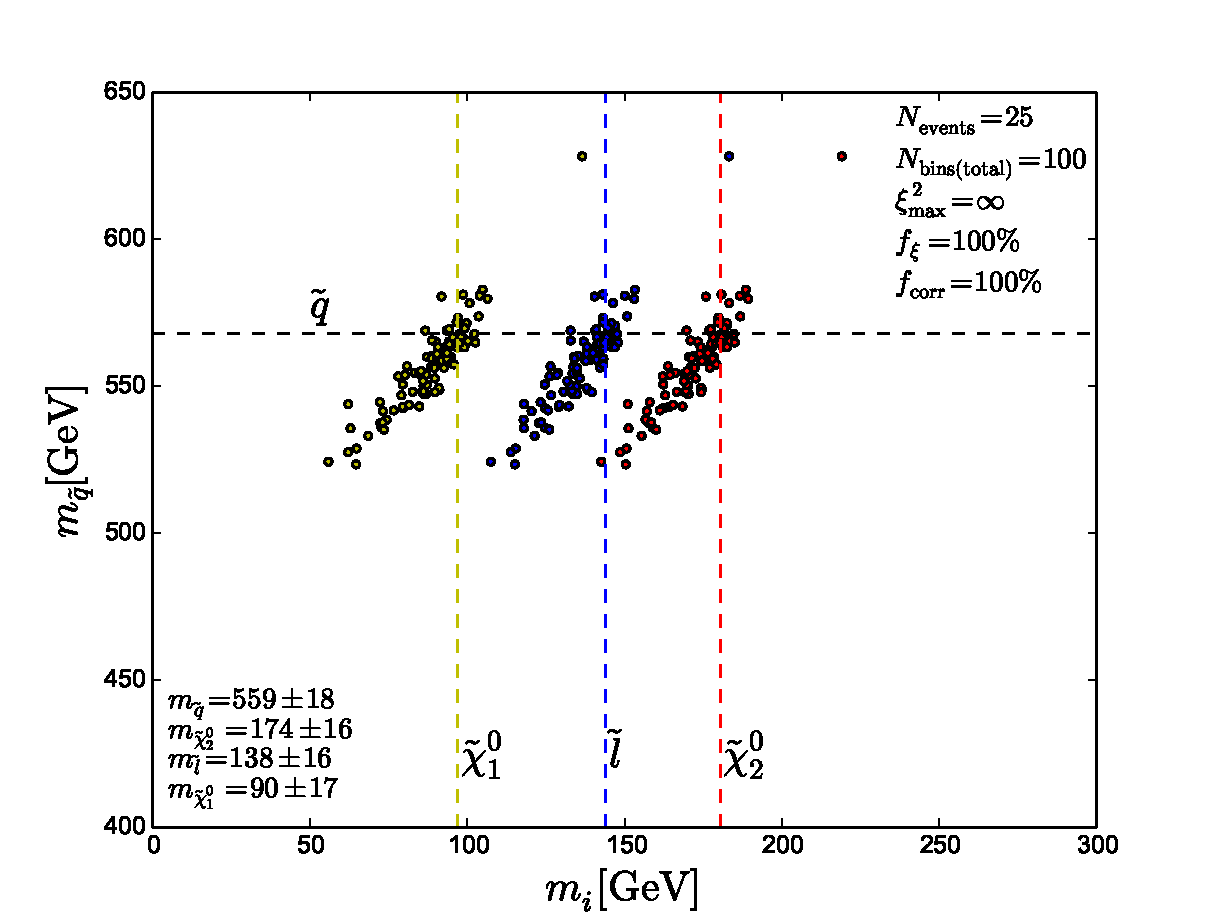
\includegraphics[width=\textwidth]{figures/improving_combinatorics/herwigpp-MD-dileptonedge-fit-nocomb-nosmear-nocut.pdf} 
		\caption{ }
		\label{fig:MD_nocomb-nosmear}
	\end{subfigure}
	\begin{subfigure}[b]{0.45\textwidth}
		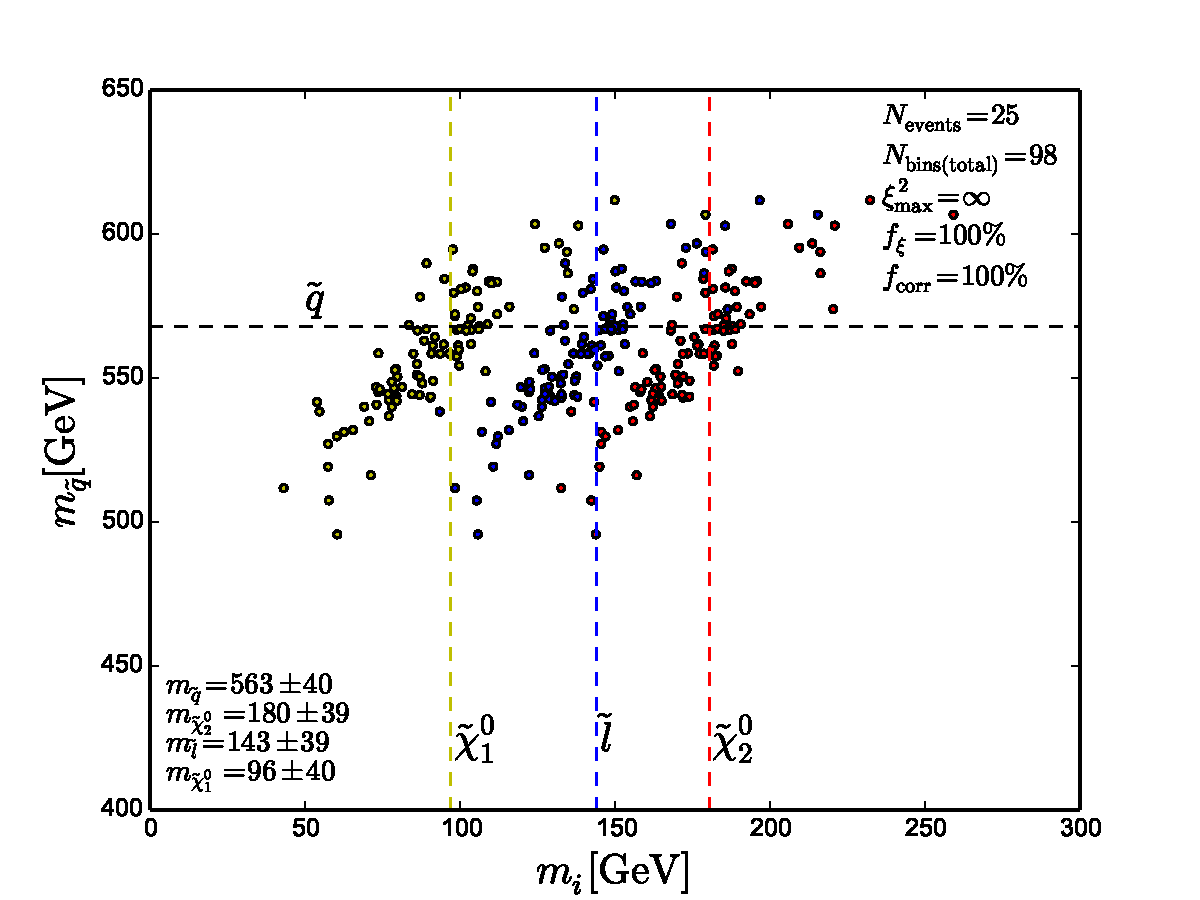
\includegraphics[width=\textwidth]{figures/improving_combinatorics/herwigpp-MD-dileptonedge-fit-nocomb-5psmear-nocut.pdf} 
		\caption{ }
		\label{fig:MD_nocomb-5psmear}
	\end{subfigure}
	\caption{Mass-difference minimizations on the Herwig++ dataset (a) without smearing and (b) with 5 \% momentum smearing, without combinatorics.}
\end{figure}
A fit of the unsmeared dataset with this method, not considering combinatorics, is shown in fig.\ \ref{fig:MD_nocomb-nosmear}. We have used the theoretical value of $m_{ll}^\mathrm{max} \approx 80 \mathrm{GeV}$ for the SPS1a masses, calculated using eq.\ \eqref{eq:invariant_mass_endpoint}. We have checked that the fit also in this case is independent of where we start the search. We also show the same fit on the dataset with 5 \% momentum smearing in fig.\ \ref{fig:MD_nocomb-5psmear}. In the last chapter we saw that with momentum smearing, the LSP mass was estimated to zero in many \marginpar{quantify} of the samples (fig. \ref{fig:moving_on-starting_point_sensitivity_no_combinatorics_5pmomsmear}) when we used the original formulation of the method. In this case all the samples have a nonzero LSP mass.
\begin{figure}[hbt]
	\centering
	\begin{subfigure}[b]{0.45\textwidth}
		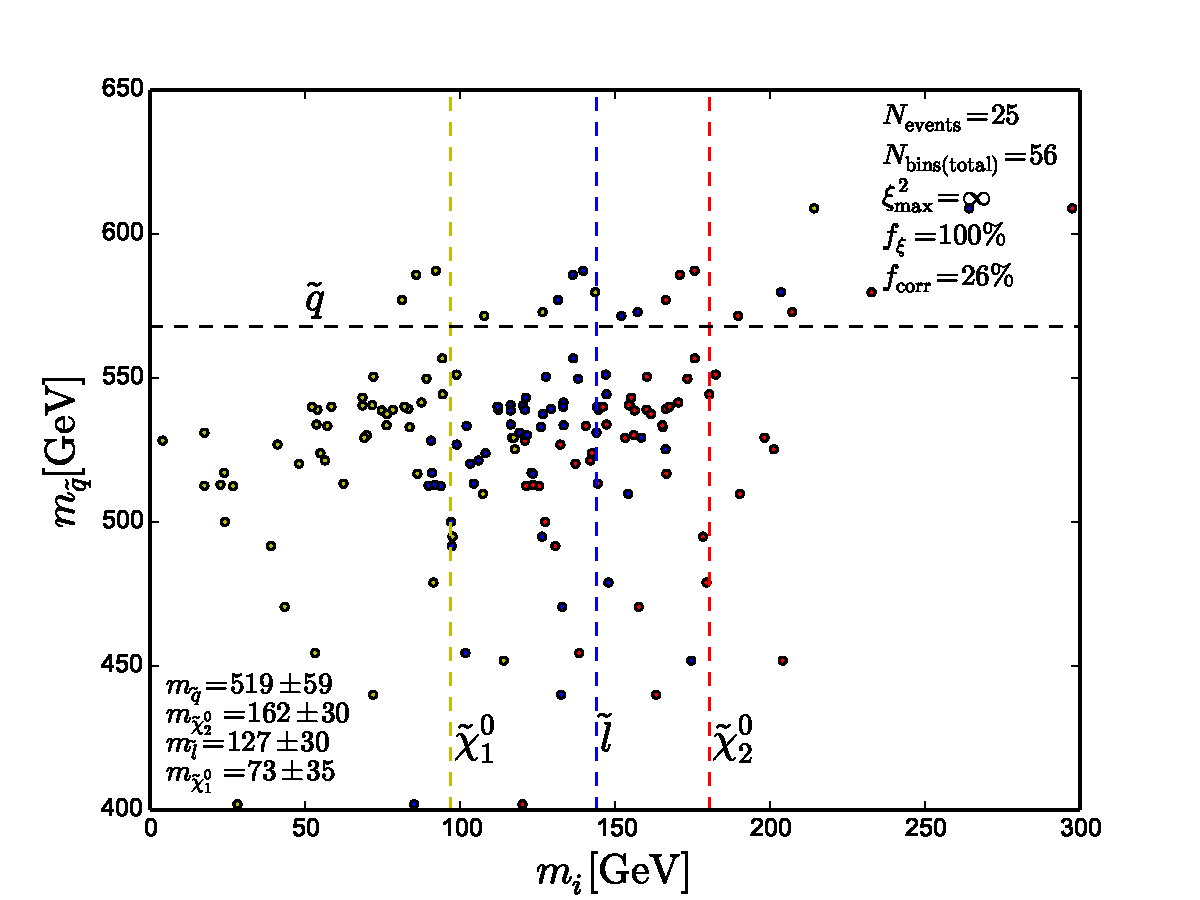
\includegraphics[width=\textwidth]{figures/improving_combinatorics/herwigpp-MD-dileptonedge-fit-comb-nosmear-nocut_TMP.pdf} 
		\caption{ }
	\end{subfigure}
	\begin{subfigure}[b]{0.45\textwidth}
		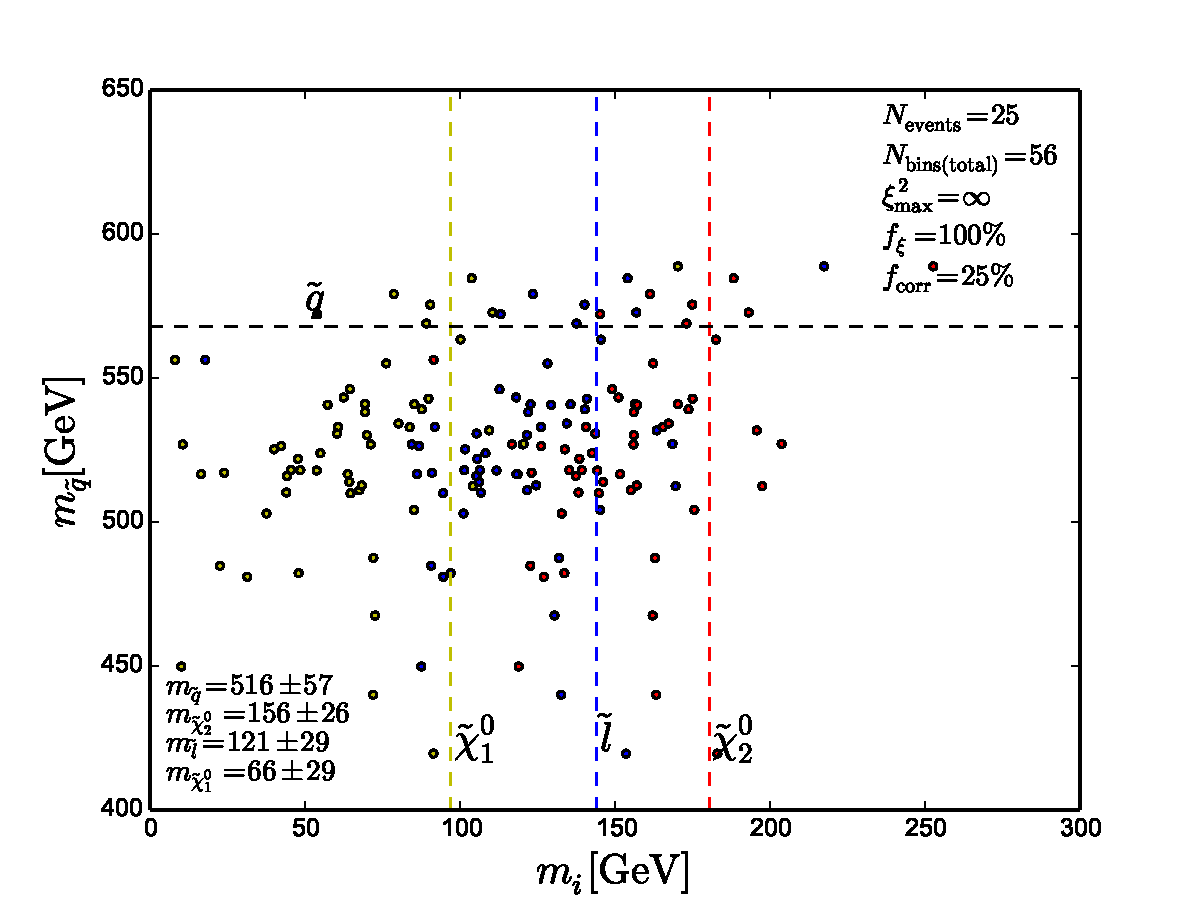
\includegraphics[width=\textwidth]{figures/improving_combinatorics/herwigpp-MD-dileptonedge-fit-comb-nosmear-nocut_400-300-200-100.pdf}
		\caption{ } 
	\end{subfigure}

	\begin{subfigure}[b]{0.45\textwidth}
		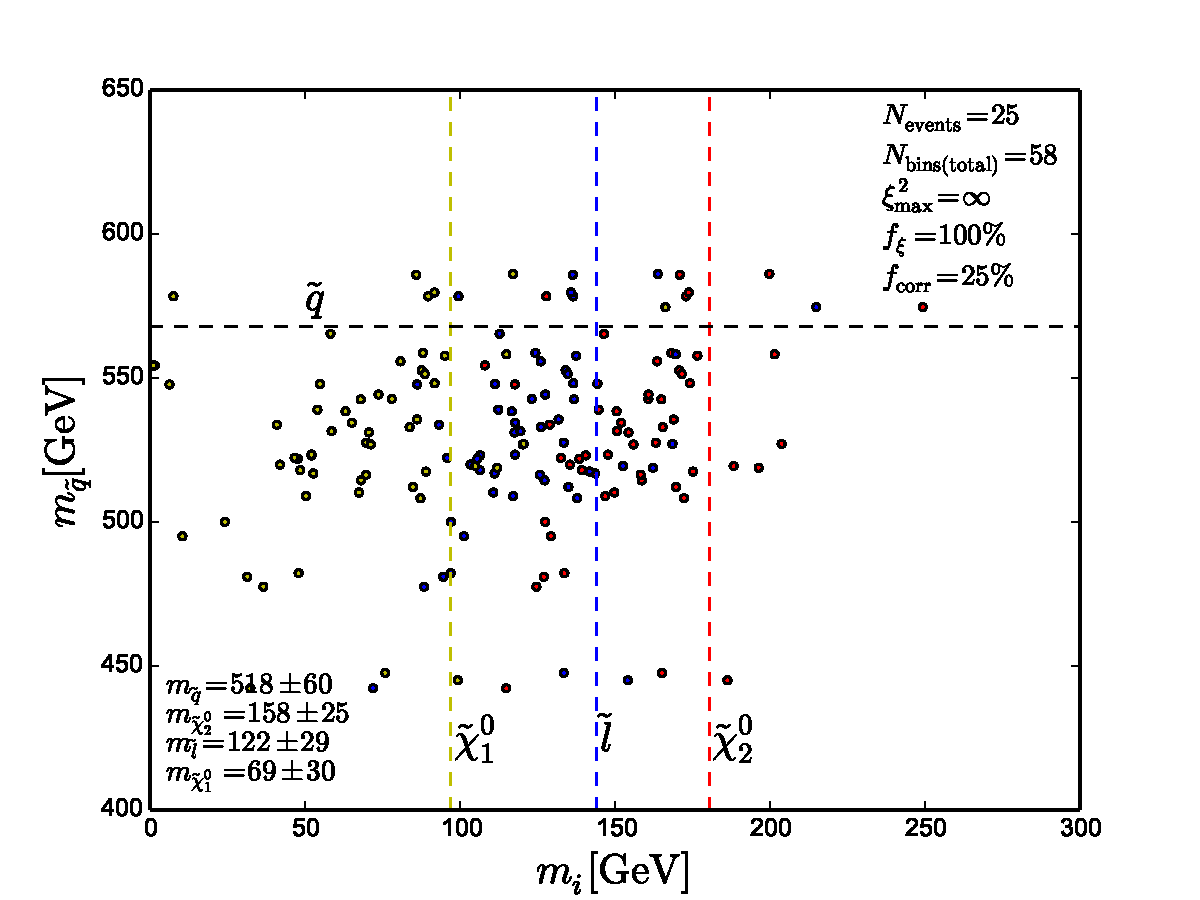
\includegraphics[width=\textwidth]{figures/improving_combinatorics/herwigpp-MD-dileptonedge-fit-comb-nosmear-nocut_800-500-300-50.pdf} 
		\caption{ }
	\end{subfigure}
	\begin{subfigure}[b]{0.45\textwidth}
		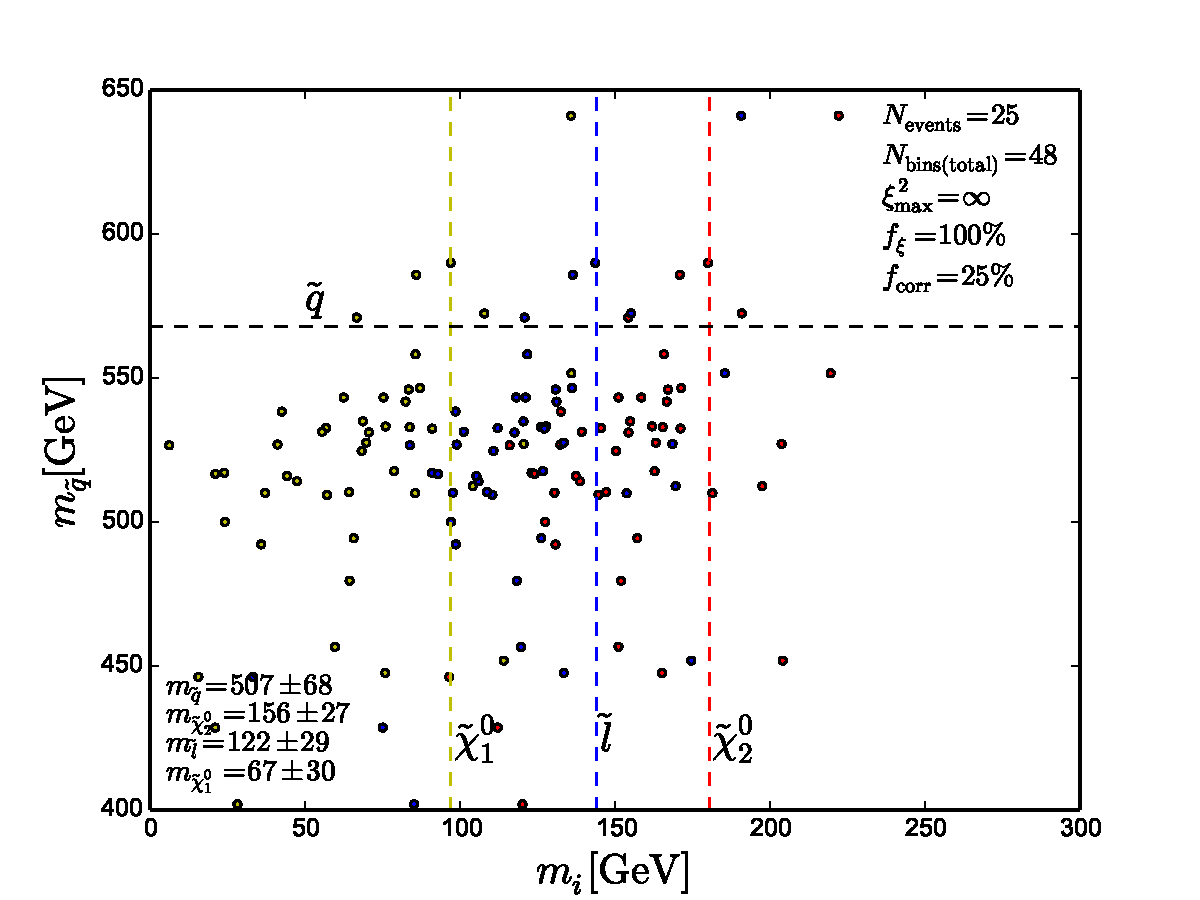
\includegraphics[width=\textwidth]{figures/improving_combinatorics/herwigpp-MD-dileptonedge-fit-comb-nosmear-nocut_1000-100-80-30.pdf}
		\caption{ } 
	\end{subfigure}
	\caption{Mass-difference minimization on the unsmeared Herwig++ dataset with combinatorics done according to Webber, for the four different starting points used earlier.}
	\label{fig:MD_starting_point_sensitivity_combinatorics}
\end{figure}
\begin{figure}[hbt]
	\centering
	\begin{subfigure}[b]{0.45\textwidth}
		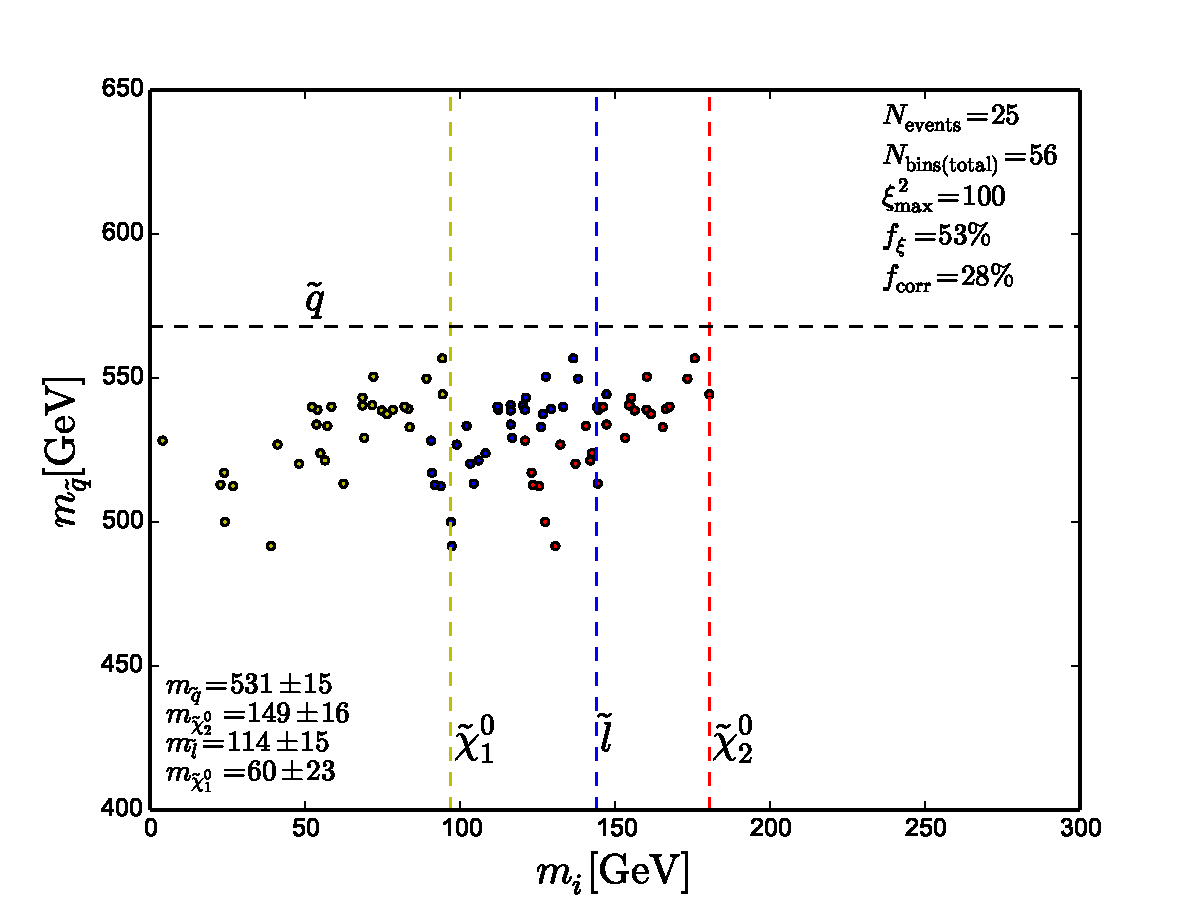
\includegraphics[width=\textwidth]{figures/improving_combinatorics/herwigpp-MD-dileptonedge-fit-comb-nosmear-cut100_TMP.pdf} 
		\caption{ }
	\end{subfigure}
	\begin{subfigure}[b]{0.45\textwidth}
		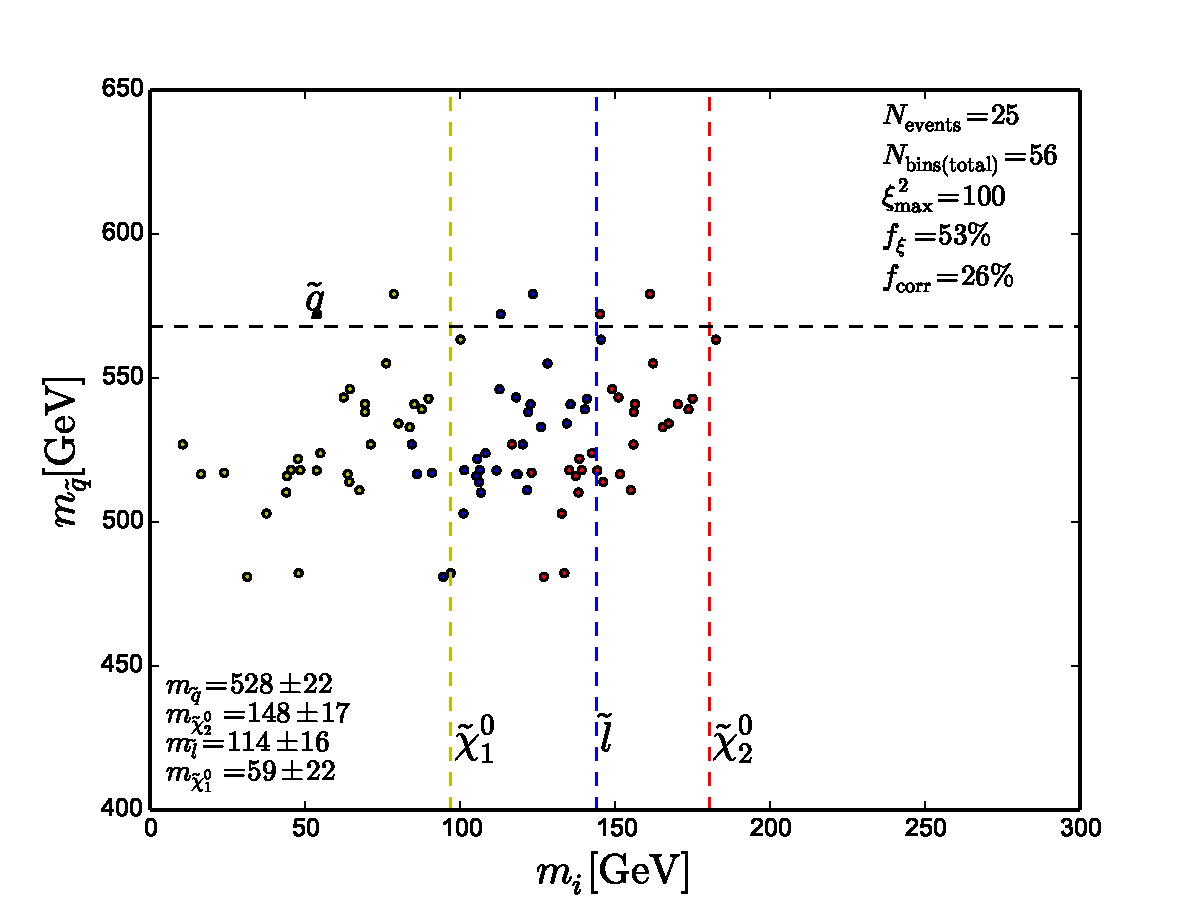
\includegraphics[width=\textwidth]{figures/improving_combinatorics/herwigpp-MD-dileptonedge-fit-comb-nosmear-cut100_400-300-200-100.pdf}
		\caption{ } 
	\end{subfigure}

	\begin{subfigure}[b]{0.45\textwidth}
		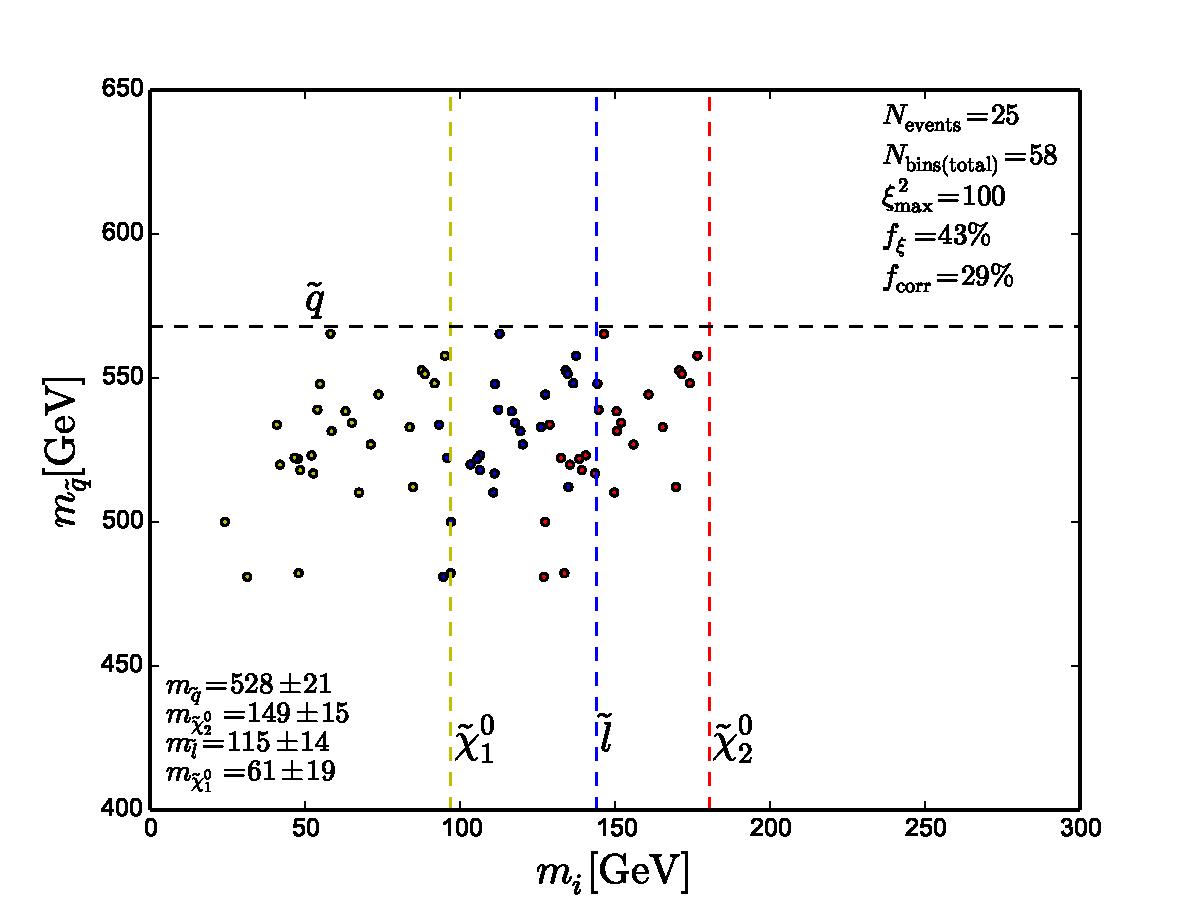
\includegraphics[width=\textwidth]{figures/improving_combinatorics/herwigpp-MD-dileptonedge-fit-comb-nosmear-cut100_800-500-300-50.pdf} 
		\caption{ }
	\end{subfigure}
	\begin{subfigure}[b]{0.45\textwidth}
		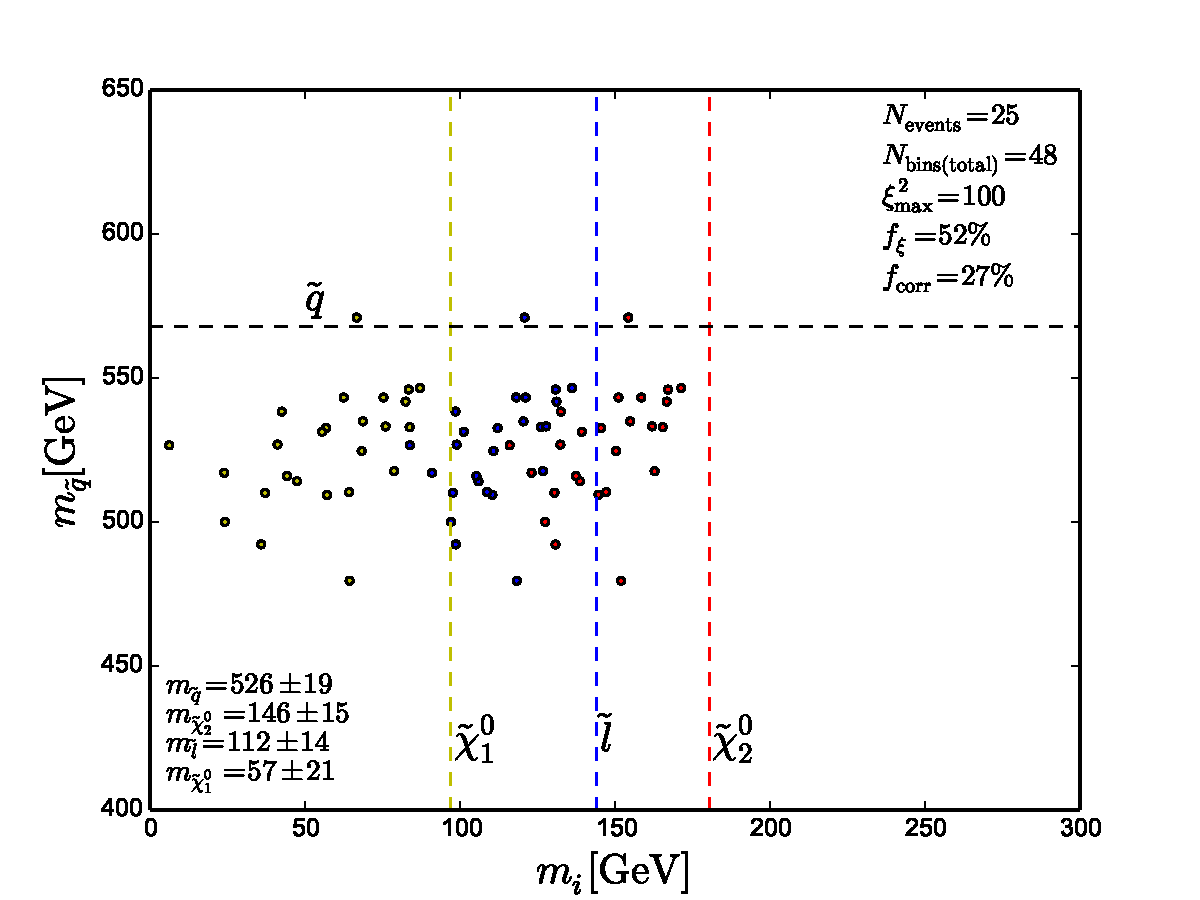
\includegraphics[width=\textwidth]{figures/improving_combinatorics/herwigpp-MD-dileptonedge-fit-comb-nosmear-cut100_1000-100-80-30.pdf}
		\caption{ } 
	\end{subfigure}
	\caption{Mass-difference minimization on the unsmeared Herwig++ dataset with combinatorics done according to Webber, for the four different starting points used earlier, subject to a $\xi^2$ cut of 100.}
	\label{fig:MD_starting_point_sensitivity_combinatorics_cut}
\end{figure}

We immediately investigate whether the modifications have affected the combinatorical problems we faced when using the original formulation, where we pick the lowest among all combinations for each event in each point. We saw in section \ref{sec:SP-dependence_webber} that the results were dependent on where the minimization search was started. In fig. \ref{fig:MD_starting_point_sensitivity_combinatorics} we show plots of the best-fit points using the same method for handling the combinatorical ambiguities, but the mass-squared-difference formulation of the $\xi^2$, minimized from the four different starting points used earlier. In fig.\ \ref{fig:MD_starting_point_sensitivity_combinatorics_cut} we show the same plots with the standard 100 GeV cut applied on the $\xi^2$. The differences between the plots appear less significant than in fig.\ \ref{fig:starting_point_sensitivity_combinatorics}. This is reflected in the mean values, which for the no-cut case range from 507 to 519 GeV in the four plots, and in the standard errors, which all are about 60 GeV. We also see that in fig.\ \ref{fig:MD_starting_point_sensitivity_combinatorics_cut}, where the cut is applied, the best-fit points surviving the cut lie in the same region in all four plots. The four different starting points are also consistent with respect to how many samples obtain convergence in the minimization (about 50 of 100), how many samples survive the $\xi^2$ cut (about 50 \% of the convergent samples), and how many events obtain the correct combinatorical choice in the best-fit point (about 25 \% of the convergent samples). \marginpar{Note: Check whether the remaining 75 \% of events are evenly divided between the other three combinations with same lepton-quark pairing!}

Statistically, the four plots in fig.\ \ref{fig:MD_starting_point_sensitivity_combinatorics} and \ref{fig:MD_starting_point_sensitivity_combinatorics_cut} are similar. But the individual event samples are not consistently fitted to the same points, and the same samples do not obtain convergence in all cases. In the case where no cut is applied, 32 of the 100 event samples obtain convergence from all four starting points, although each starting point has about 50 convergent samples. Only three of the samples obtain best-fit points less than $0.1$ GeV apart in all four masses in all four cases. The standard error between the four best-fit points for each event sample has an average of between 10 and 15 GeV for the four masses.\marginpar{Does this sentence make sense? Also, do the same analysis for the case with xisquared-cut.}



\section{Summing the combinations}
\label{sec:combinatorics-sum_all_contributions}
We have seen that when we minimize only the true combinatorical choice, the minimization is independent of starting point. If we include all combinations by always selecting the lowest among the values in each point, a starting-point dependence is introduced. The mathematical difference between these two problems is that in the former case, the $\xi^2$ is a smooth polynomial, while in the latter case it is not smooth. We can make the $\xi^2$ surface smooth if we add the different combinatorical choices together instead of choosing between them. Webber mentions this option in his article, but discards it, saying {\it ``The surface would be smooth if one added the $\xi^2$ contributions of all combinations,  but then the sensitivity to the correct solution is reduced and biases are introduced by the huge contributions of wrong combinations''} \cite{Webber:2009vm}. However, not all combinations will contribute equally if they are included. In \cite{Gripaios:2011jm} it is pointed out that some of the wrong combinations will tend to give reconstructions close to the true combinations. \marginpar{Discuss some more? What is the argument? What do they actually say?}

For the case where the dileptons differ in generation between the chains, which is what we have used in our analysis thus far, there are eight combinatorical possibilities. These can be divided into two categories depending on which lepton pair is paired with which quark. For each of these pairings, there are four combinations of near and far leptons. The matrix $\mathbf{A}$ is invariant, up to a permutation of rows, for each of the two categories. If we add all four combinations of near and far leptons for each event to the $\xi^2$, then the problem reduces from an eight-fold ambiguity to a two-fold ambiguity. 
\begin{figure}[hbt]
	\centering
	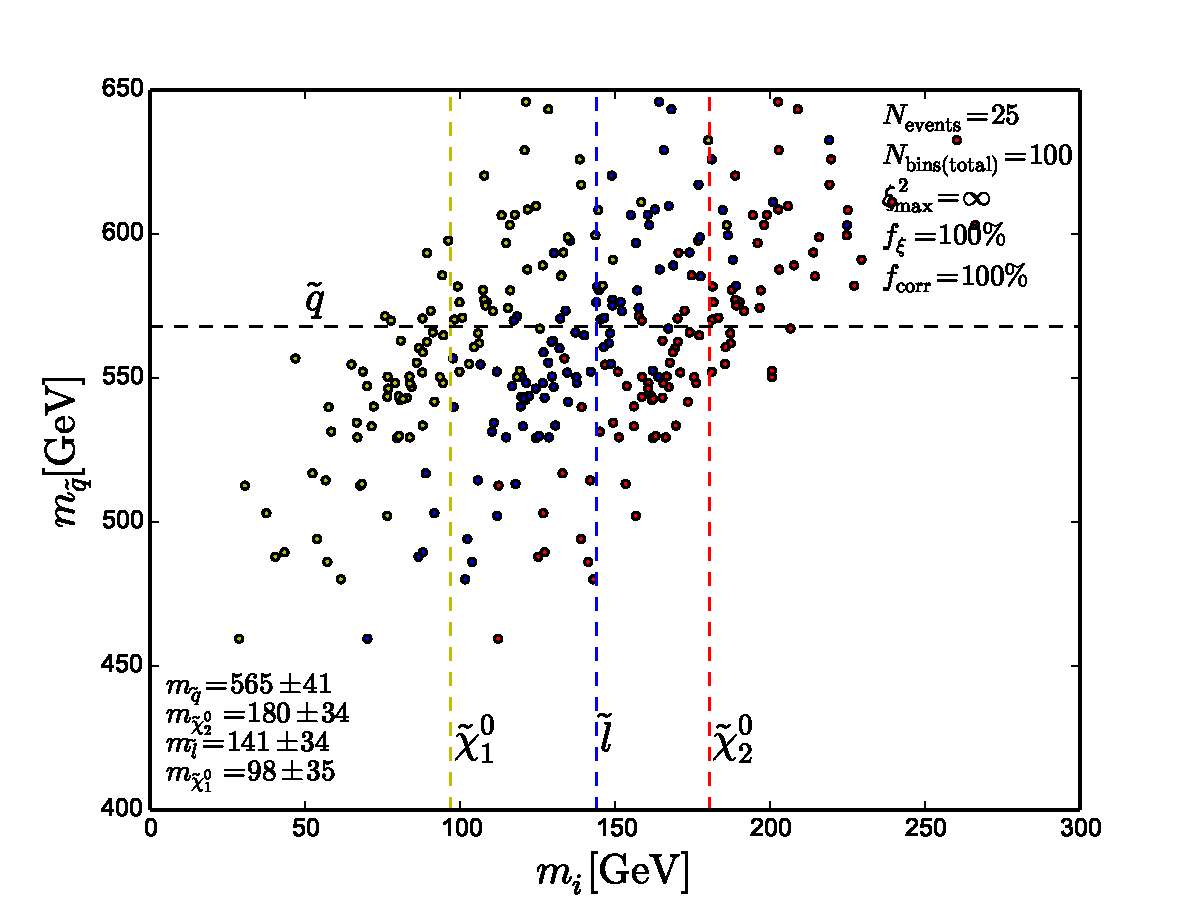
\includegraphics[width=0.8\textwidth]{figures/improving_combinatorics/herwigpp-4combosum-fit-nocomb-nosmear-nocut.pdf} 
	\caption{Minimization of the unsmeared {\tt Herwig++} dataset where all orderings of the leptons within the same chains are included.}
	\label{fig:4combosum_nocomb-nosmear}
\end{figure}
In fig.\ \ref{fig:4combosum_nocomb-nosmear} we show a fit of the unsmeared dataset where the $\xi^2$ has been constructed in this way, but where only the true pairing of quarks and leptons is considered. The mean values and standard errors for the mass fits in the 100 samples is $565 \pm 41\, \mathrm{GeV}, 180 \pm 34\, \mathrm{GeV}, 141 \pm 34\, \mathrm{GeV}$ and $98 \pm 35\, \mathrm{GeV}$, respectively. The standard error is quite large, about 40 GeV for all the four masses, but the mean values are very close to the true values in all four cases -- there is no bias. The minimization is also completely robust against starting points: For the four different starting points used earlier, all 100 bins obtain convergence in all cases, and each sample is fitted to the same point in all cases. \marginpar{The number of samples that converge is an important factor, 100 \% here vs 50 \% in the webber-jumping.}

\begin{figure}[hbt]
	\centering
	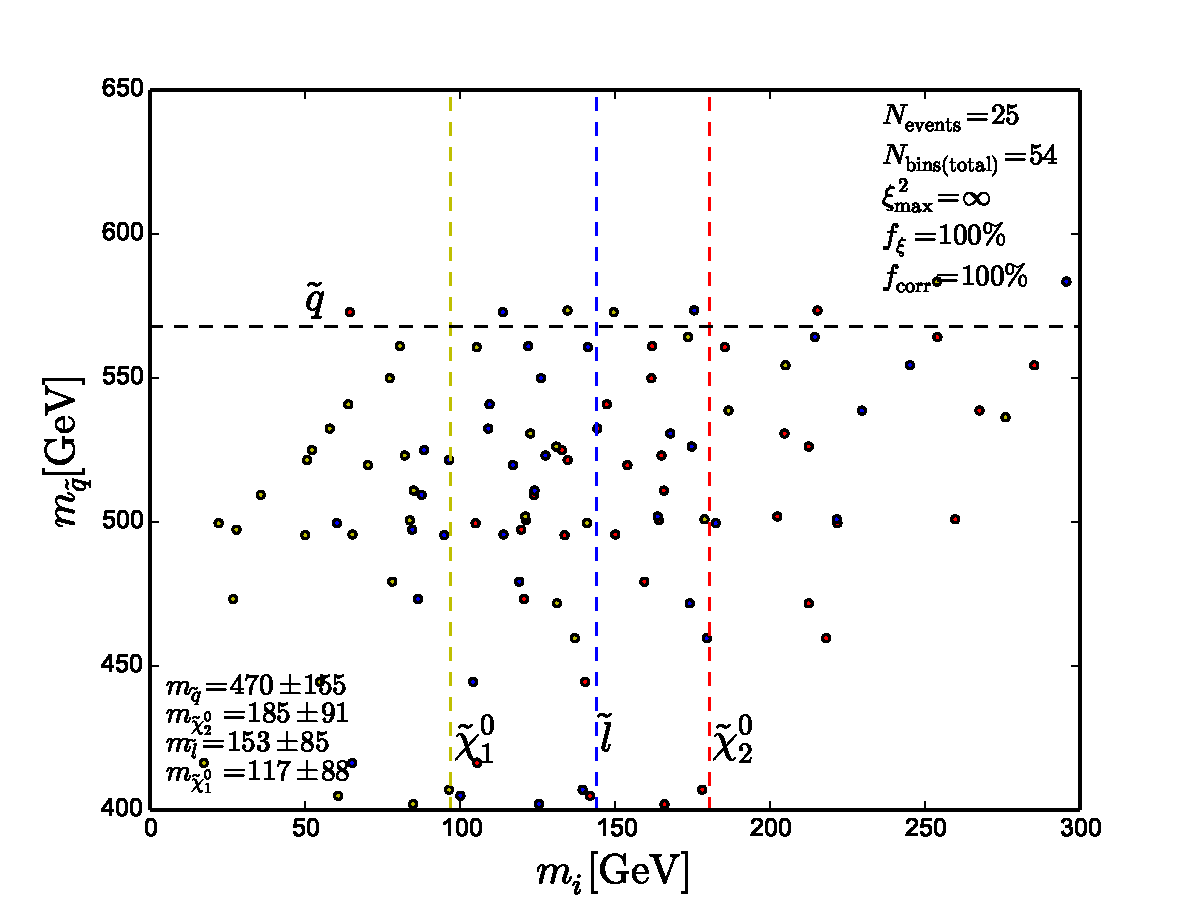
\includegraphics[width=0.8\textwidth]{figures/improving_combinatorics/herwigpp-8combosum-fit-nosmear-nocut.pdf} 	
	\caption{Minimization of the unsmeared {\tt Herwig++} dataset where all eight combinations are included.}
	\label{fig:8combosum-nosmear}
\end{figure}
If we include all eight combinations instead of only the four closest, then the results worsen considerably. This is shown in fig.\ \ref{fig:8combosum-nosmear}. While the robustness against starting points is retained, only half of the samples obtain convergence, and the errors on the masses are about 90 GeV for the three lightest particles and 150 GeV for the squark. There is a significant downward bias on the squark mass.

We proceed with investigating the method of summing only the four closest combinations. In this formulation, there are several options for handling the remaining two-fold combinatorical ambiguity. One option is to utilise the original method of ``jumping'' between values, always selecting the lowest among the combinations for each event at each mass point. When there are just two different values to choose between, the amount of jumping and the resulting difficulties might be reduced. We check this by starting the minimization from the four different starting points. We find in this case for the unsmeared dataset that $\sim 90$ samples converge in each case, while 84 of the samples converge in all four cases. 62 of the samples are fitted consistently, meaning that all four minimization agree on all four mass values within 0.1 GeV. The mean standard error on the best-fit points from the four different minimizations in the 84 samples is 9 GeV for the squark and about 4 GeV for the other three masses. We also find that about 80 \% of the events obtain the minimum with the correct combination, while the remaining 20 \% apparently obtain smaller values using the wrong combination of quarks and leptons.
\begin{figure}[hbt]
	\centering
	\begin{subfigure}[b]{0.45\textwidth}
		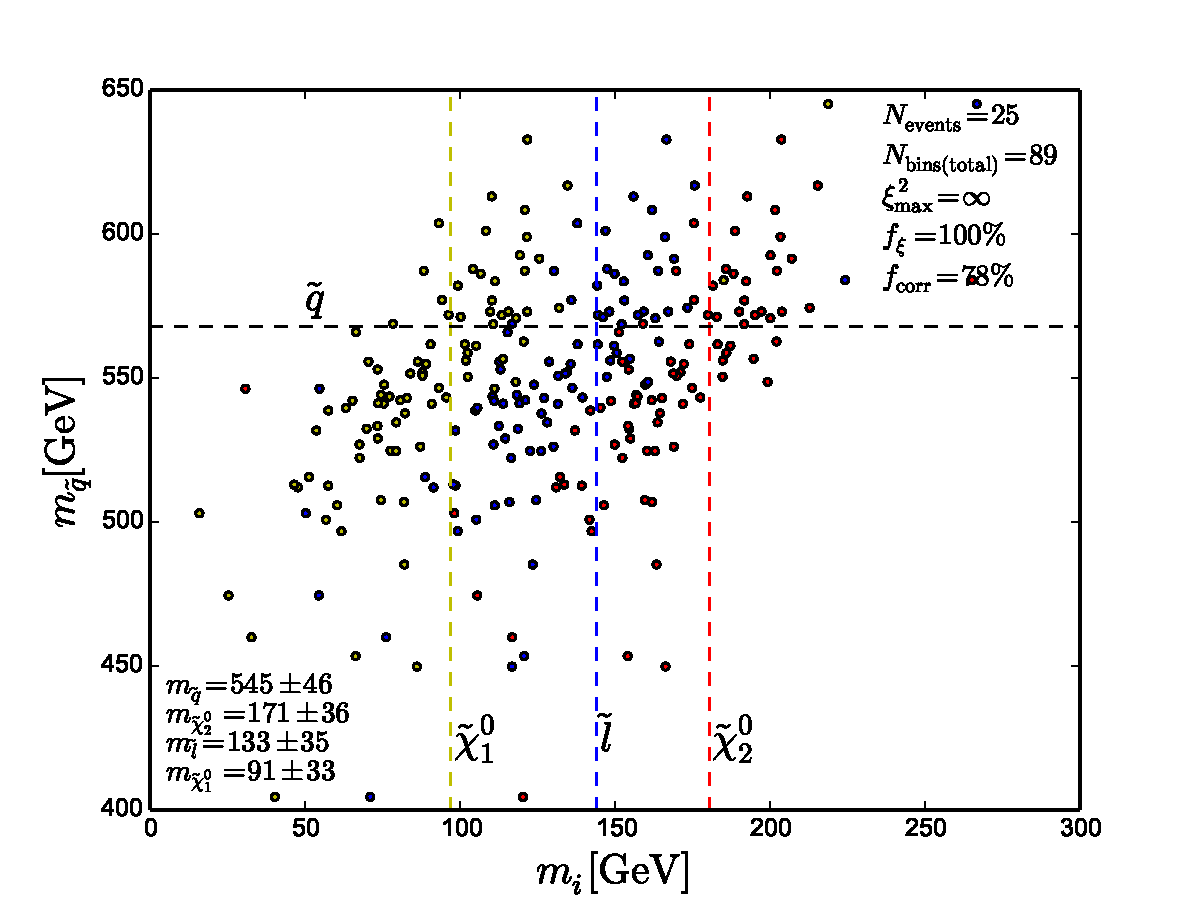
\includegraphics[width=\textwidth]{figures/improving_combinatorics/herwigpp-4combosum-fit-jump_comb-nosmear-nocut-TMP.pdf} 
		\caption{ }
	\end{subfigure}
	\begin{subfigure}[b]{0.45\textwidth}
		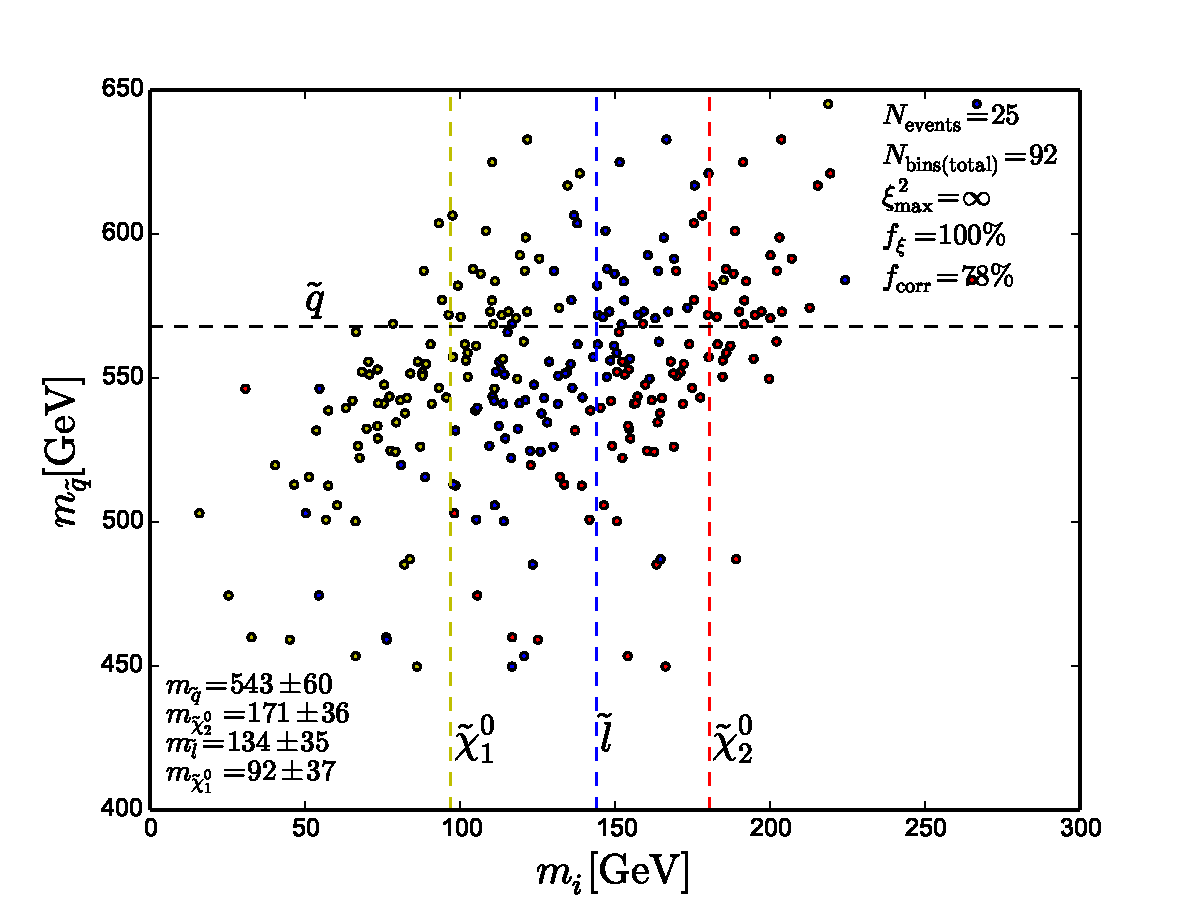
\includegraphics[width=\textwidth]{figures/improving_combinatorics/herwigpp-4combosum-fit-jump_comb-nosmear-nocut-400-300-200-100.pdf}
		\caption{ } 
	\end{subfigure}

	\begin{subfigure}[b]{0.45\textwidth}
		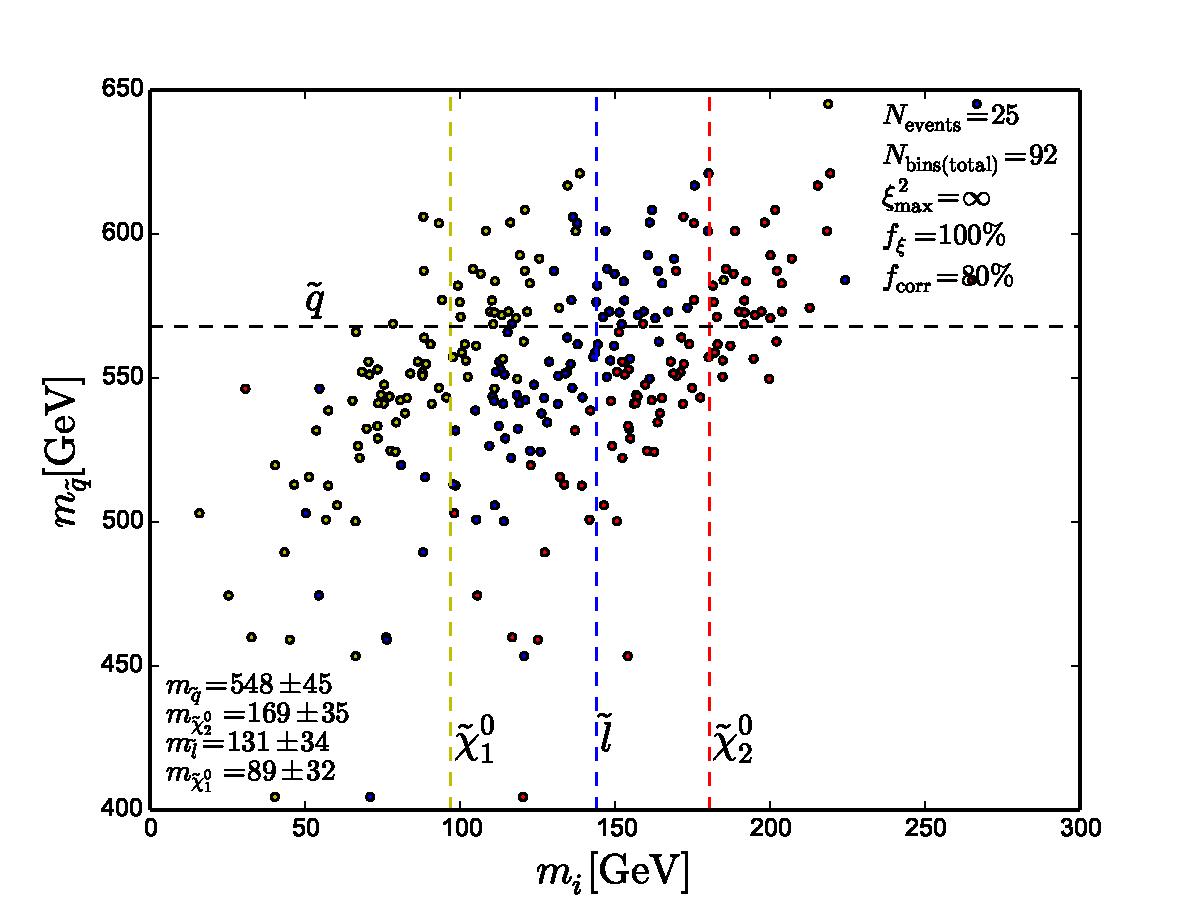
\includegraphics[width=\textwidth]{figures/improving_combinatorics/herwigpp-4combosum-fit-jump_comb-nosmear-nocut-800-500-300-50.pdf} 
		\caption{ }
	\end{subfigure}
	\begin{subfigure}[b]{0.45\textwidth}
		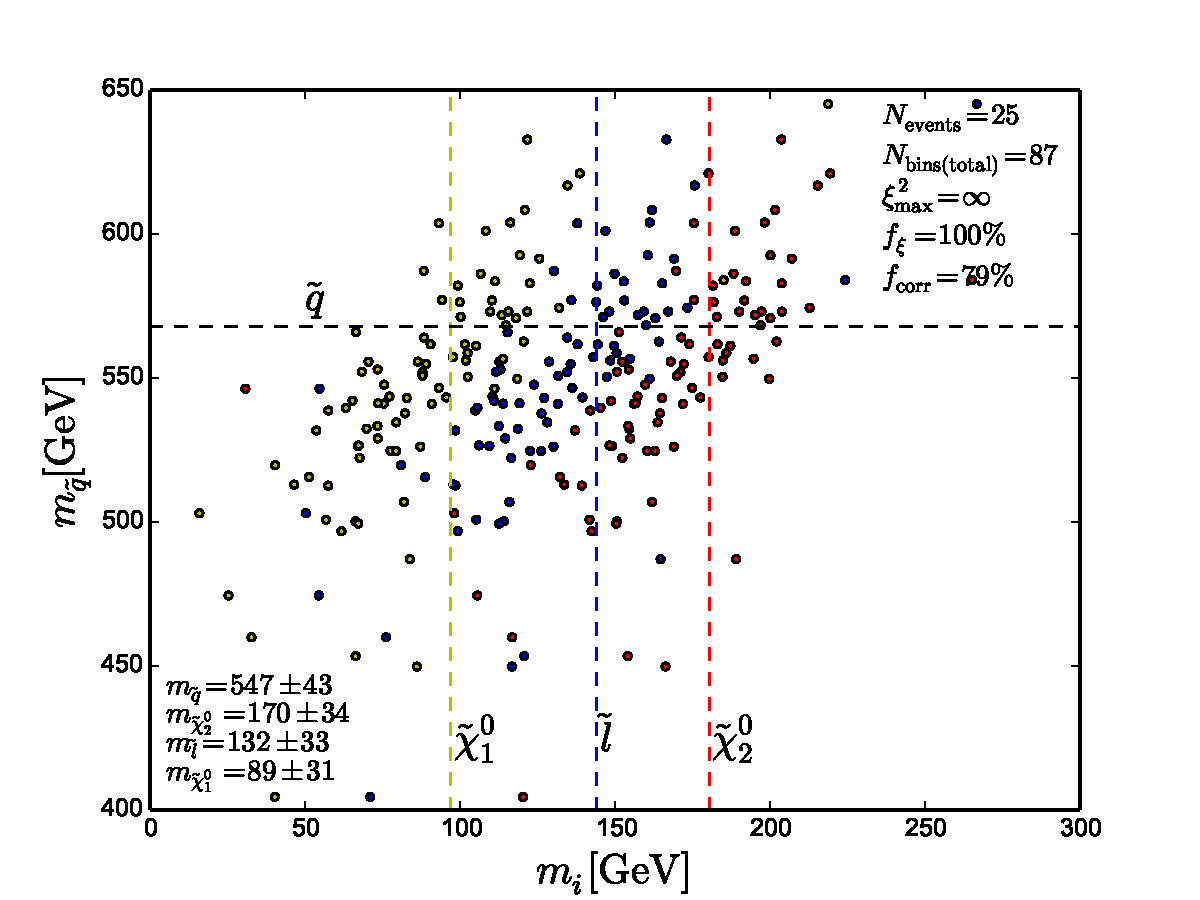
\includegraphics[width=\textwidth]{figures/improving_combinatorics/herwigpp-4combosum-fit-jump_comb-nosmear-nocut-1000-100-80-30.pdf}
		\caption{ } 
	\end{subfigure}
	\caption{Mass-difference minimization on the unsmeared Herwig++ dataset with combinatorics handled by summing the four closest combinations and jumping between the two quark-lepton combinations, for the four different starting points used earlier.}
	\label{fig:4combosum_starting_point_sensitivity_combinatorics-jumping}
\end{figure}

Another possibility is to combine a few events at a time, and minimize the $\xi^2$, with the lepton-combinations summed, separately for each of the quark-lepton combinations ({\it e.g.}\ each matrix $\mathbf{A}$) in each event. For instance, if we select two events, then there are four ways to combine the different $\mathbf{A}$ matrices among the events. If the lowest $\xi^2$ minimum value among these four tend to belong to the true $\mathbf{A}$ matrices, then this may be used to select the correct quark-lepton combinations before all events are summed together for the total mass fit. \marginpar{A BIG IF: Test if this actually works.}





\begin{itemize}
\item Smooth minimization, finds same minimum always. Include plot showing this?
\item Compare mean value and error to the original hopes of Webber, and to e.g. Cheng. 
\item However, biased. Cite cheng, wrong combinations bias downward. Desireable to reduce wrong combinations also within same matrix.
\item Investigate determinant.
\item Investigate SFL events. What happens to the minima if there are four different A matrices? Can we select the true combo among the four? Remember to also utilise the dilepton edge to discriminate.
\item Possible way out of combinatorics: Sum all contributions with same matrix A. Select between the two matrices in some way, either by Webber-jumping or by selecting on samples of fewer events. That actually works better than I thought. At LEAST something to include plots of. Note: Bias toward lower values, even after cut. Can be corrected by MC? 
\item A point for conclusions: Webber cites the Cheng papers in the original article, pointing out that his method is ``closest in spirit to those''. So maybe we can sum up by comparing, and saying something about that the Cheng version appears to have prospects for a more accurate determination?
\end{itemize}




















\clearpage
\section{The pile}



We saw in the previous chapter that the minimization was not well-defined, since it depended heavily on the choice of starting point. This was however a minimization done with the full inclusion of combinatorical ambiguities (see section \ref{sec:combinatorics}). While these ambiguities are clearly unavoidable -- we do not know \`{a} priori which particles belong together -- there may be other ways to handle them than the intuitive method applied in the above analysis. It might be possible to use other kinematical constraints, like the end-point method mentioned in section \ref{ch:introducing_the_method}, to rule out combinations. We could also try to minimize a separate $\xi^2$ for each combination in each event, and select the combination which gives the lowest value as the true one -- {\bf if} this turns out to correlate with the correct combination. In \cite{Gripaios:2011jm} there is a comprehensive discussion of the relationship between different combinations -- maybe we can exploit these relationships to pin down the correct combination? Or borrow some other ideas from it?

We should also investigate methods to identify events which contribute badly to the fit, so they can be dropped. We might try to use the event-wise $\xi^2$ for this, dropping events with a large minimum. We could also hope to use the determinant of the matrix A to identify events that are difficult to invert (small determinant), surmising that they also will give poor reconstruction. We should also investigate the determinant for the different combinatorical choices -- maybe we can rule out some combinations based on this? (Although several combinations share the same A.)

Below it turns out that the method seems insensitive to the LSP mass -- I am starting to think that the way they do it in \cite{Nojiri:2010dk}, fitting the squared mass differences instead, is all we can hope to do. But this should be tried together with using the dilepton end-point to pin the LSP mass, which MAY give a full reconstruction again. Or at least some more plots.




\begin{itemize}
	\item Minimize separately for each event? Do something to make it steep enough?
	\item combinatorical elimination: momentum cuts, angles, invariant mass edge. Angular selection: squarks produced more or less at rest (except if they come from gluino in a large mass-gap scenario). But if there is a mass gap further down, does this give anisotropies in angular distributions of opposite-chain particles? Don't focus on angles.
	\item migrad or similar for minimization of 1-event bins? Provide gradient, analytical or numerical?
	\item combinatorical issues with three or four hard squarks -- gluino-gluino vs gluino-squark vs squark-squark/squark-antisquark. Nllfast to give xsec. 
	\item Examine correlation between det(A) and minimization performance. 
	\item Include plots of the $\xi^2$ surface somewhere suitable -- maybe we can even compare combinatorics vs no combinatorics in a nice way?
\end{itemize}















































% %%%%%%%%%%%%%%%%%%%%%%%%%%%%%%%%%%%%%%%%
% \chapter{Improvements of the method}
% %%%%%%%%%%%%%%%%%%%%%%%%%%%%%%%%%%%%%%%
% To think about: How do we scan when we don't know true values? The fit is sensitive to initial values. Might it be fruitful to run many minimizations with different starting positions? That would essentially stack another 4-dimensional minimization on top of this one. Would scale CPU time enormously. Probably not that clever.

% What about discarding events with large minima? Do they seem to ruin the fit or is the minimal value not that good a measurement? Webber does this. 

% I have not looked much into using Det(A) as a measure of invertibility. It seems like invertibility is not really the big issue, but it might be worth investigating never the less. Maybe discard events based on Det(A)?

% One very unchewed idea: How about fitting the more fundamental SUSY soft parameters instead of the physical masses? I.e. substitute the soft masses instead of the physical ones? Can we gain something under different model assumptions, extract some co-varying parameters or something?






















\appendix

\chapter{A C++ implementation of the Nelder-Mead Simplex algorithm}
\label{ch:simplex}

The function to call for minimization is {\tt amoeba}. It returns true or false depending on whether convergence has been obtained within the set number of iterations.

\lstset{language=C++}
\begin{lstlisting}
	// Implementation of Nelder-Mead Simplex method:
double * alloc_vector(int cols)
{
	return (double *) malloc(sizeof(double) * cols);
}
void free_vector(double * vector , int cols)
{
	free(vector);
}
double ** alloc_matrix(int rows, int cols)
{
	int	i;
	double ** matrix = (double **) malloc(sizeof(double *) * rows);
	for (i = 0; i < rows; i++)
		matrix[i] = alloc_vector(cols);
	return matrix;
}
void free_matrix(double ** matrix, int rows, int cols)
{
	int	i;
	for (i =0; i < rows; i++)
		free_vector(matrix[i], cols);
	free(matrix);
}
double ** make_simplex(double * point, int dim)
{
	int i, j;
	double ** simplex = alloc_matrix(dim + 1, dim);
	for (i = 0; i < dim + 1; i++)
		for (j = 0; j < dim; j++)
			simplex[i][j] = point[j];
	for (i = 0; i < dim; i++)
		// simplex[i][i] += 1.0;
		simplex[i][i] *= 1.1;
	return simplex;
}
void evaluate_simplex(double ** simplex, int dim,double * fx,  double (*func)(double *, int, int, double, bool, vector<bool> &, vector<vector<mat>> &, vector<vector<vec>> &, vector<bool> &),
	int Nevents, int jBin, double Mnorm, bool combinatorics, vector<bool> &all_leptons_equal_list, vector<vector<mat>> &D_lists, vector<vector<vec>> &E_lists, vector<bool> &correct_combinatorics)
{
	int i;
	for (i = 0; i < dim + 1; i++)
	{
		correct_combinatorics.clear();
		fx[i] = (*func)(simplex[i], Nevents, jBin, Mnorm, combinatorics, all_leptons_equal_list, D_lists, E_lists, correct_combinatorics);
	}
}

void simplex_extremes(double *fx, int dim, int & ihi, int & ilo,int & inhi)
{
	int i;
	if (fx[0] > fx[1])
	{ ihi = 0; ilo = inhi = 1; }
	else
	{ ihi = 1; ilo = inhi = 0; }
	for (i = 2; i < dim + 1; i++)
		if (fx[i] <= fx[ilo])
			ilo = i;
		else if (fx[i] > fx[ihi])
			{ inhi = ihi; ihi = i; }
		else if (fx[i] > fx[inhi])
			inhi = i;
}
void simplex_bearings(double ** simplex, int dim,double * midpoint, double * line, int ihi)
{
	int i, j;
	for (j = 0; j < dim; j++)
		midpoint[j] = 0.0;
	for (i = 0; i < dim + 1; i++)
		if (i != ihi)
			for (j = 0; j < dim; j++)
				midpoint[j] += simplex[i][j];
	
	for (j = 0; j < dim; j++)
	{
		midpoint[j] /= dim;
		line[j] = simplex[ihi][j] - midpoint[j];
	}
}
int update_simplex(double * point, int dim, double & fmax,double * midpoint, double * line, double scale, double (*func)(double *, int, int, double, bool, vector<bool> &, vector<vector<mat>> &, vector<vector<vec>> &, vector<bool> &),
	int Nevents, int jBin, double Mnorm, bool combinatorics, vector<bool> &all_leptons_equal_list, vector<vector<mat>> &D_lists, vector<vector<vec>> &E_lists, vector<bool> &correct_combinatorics)
{
	int i, update =	0; 
	double * next = alloc_vector(dim), fx;
	for (i = 0; i < dim; i++)
		next[i] = midpoint[i] + scale * line[i];
	correct_combinatorics.clear();
	fx = (*func)(next, Nevents, jBin, Mnorm, combinatorics, all_leptons_equal_list, D_lists, E_lists, correct_combinatorics);
	if (fx < fmax)
	{
		for (i = 0; i < dim; i++)	
			point[i] = next[i];
		fmax = fx;
		update = 1;
	}
	free_vector(next, dim);
	return update;
}

void contract_simplex(double ** simplex, int dim, double * fx, int ilo, double (*func)(double *, int, int, double, bool, vector<bool> &, vector<vector<mat>> &, vector<vector<vec>> &, vector<bool> &),	int Nevents, int jBin, double Mnorm, bool combinatorics, vector<bool> &all_leptons_equal_list, vector<vector<mat>> &D_lists, vector<vector<vec>> &E_lists, vector<bool> &correct_combinatorics)
{
	int i, j;
	for (i = 0; i < dim + 1; i++)
		if (i != ilo)
		{
			for (j = 0; j < dim; j++)
				simplex[i][j] = (simplex[ilo][j]+simplex[i][j])*0.5;
			correct_combinatorics.clear();
			fx[i] = (*func)(simplex[i], Nevents, jBin, Mnorm, combinatorics, all_leptons_equal_list, D_lists, E_lists, correct_combinatorics);
		}
}


#define ZEPS 1e-30
int check_tol(double fmax, double fmin, double ftol)
{
double delta = fabs(fmax - fmin);
double accuracy = (fabs(fmax) + fabs(fmin)) * ftol;
// cout << delta << ", " << accuracy << ", " << ftol << endl;
return (delta < (accuracy + ZEPS));
}

bool amoeba(double *point, double &fmin, double (*func)(double *, int, int, double, bool, vector<bool> &, vector<vector<mat>> &, vector<vector<vec>> &, vector<bool> &), 
	double tol, int maxiter,
	int Nevents, int jBin, double Mnorm, bool combinatorics, vector<bool> &all_leptons_equal_list, vector<vector<mat>> &D_lists, vector<vector<vec>> &E_lists, vector<bool> &correct_combinatorics)
{
	// Usage: Point is an allocated dim-dimensional array of doubles
	// to be filled with coordinates of the best-fit point,
	// func is the function to minimize. 
	int dim = 3; // MODIFIED TO FIT MD
	int ihi, ilo, inhi, j;
	// double fmin;
	double * fx = alloc_vector(dim + 1);
	double * midpoint = alloc_vector(dim);
	double * line = alloc_vector(dim);
	double ** simplex = make_simplex(point, dim);
	evaluate_simplex(simplex, dim, fx, func, 
		Nevents, jBin, Mnorm, combinatorics, all_leptons_equal_list, D_lists, E_lists, correct_combinatorics);

	int iter = 0;
	while (iter < maxiter)
	{
		simplex_extremes(fx, dim, ihi, ilo, inhi);
		simplex_bearings(simplex, dim, midpoint, line, ihi);
		if (check_tol(fx[ihi], fx[ilo], tol)) { /*cout << "below tol = " << tol << endl;*/ break; }
		update_simplex(simplex[ihi], dim, fx[ihi],
		midpoint, line, -1.0, func, 
		Nevents, jBin, Mnorm, combinatorics, all_leptons_equal_list, D_lists, E_lists, correct_combinatorics);
		if (fx[ihi] < fx[ilo])
			update_simplex(simplex[ihi], dim, fx[ihi], midpoint, line, -2.0, func,
				Nevents, jBin, Mnorm, combinatorics, all_leptons_equal_list, D_lists, E_lists, correct_combinatorics);
		else if (fx[ihi] >= fx[inhi])
			if (!update_simplex(simplex[ihi], dim, fx[ihi], midpoint, line, 0.5, func, Nevents, jBin, Mnorm, combinatorics, all_leptons_equal_list, D_lists, E_lists, correct_combinatorics))
				contract_simplex(simplex, dim, fx, ilo, func, Nevents, jBin, Mnorm, combinatorics, all_leptons_equal_list, D_lists, E_lists, correct_combinatorics);
		iter += 1;
	}

	for (j = 0; j < dim; j++)
		point[j] = simplex[ilo][j];
	fmin = fx[ilo];
	free_vector(fx, dim);
	free_vector(midpoint, dim);
	free_vector(line, dim);
	free_matrix(simplex, dim + 1, dim);

	if (iter < maxiter)
	{
		return true;
	}
	else
		return false;
}
\end{lstlisting}








%%%%%%%%%%%%%%%%%%%%%%%%%%%%%%%%%%%%%%%%%%%%%%%%%%%%%%%%%%%%%%%%%
\chapter{An algorithm for generating on-shell two-body decays}
%%%%%%%%%%%%%%%%%%%%%%%%%%%%%%%%%%%%%%%%%%%%%%%%%%%%%%%%%%%%%%%%%
\label{ch:decayalgorithm}

 The particles will go back-to-back in the rest frame of the decaying particle - the direction is drawn randomly from a uniform spherical distribution. This can be achieved in spherical coordinates by the assignments
\begin{align}
	U, V &= \text{uniform}(0,1)\nonumber \\
	\phi &= 2\pi U\\
	\theta &= \arccos(2V-1) \nonumber
\end{align}
The decay algorithm, in python notation, is as follows. Particle 1 of 4-momentum $p_1$ decays to particle 2 and 3 of 4-momentum $p_2$ and $p_3$.

\lstset{language=Python} 
\begin{lstlisting}
	# Calculating four-momenta of particle 2&3 going back-to-back from
	# decay of particle 1 in the frame where particle 1 has 4-mom P1
	#
	#
	# particle 1 = decaying particle
	# particle 2 & particle 3 = decay products
	# primed system is rest frame of particle 1, unprimed is lab frame
	# rotated system is at rest in lab system,
	# but rotated so particle one goes in +x direction
	p1 = P1[0,1:4]
	p1abs = np.sqrt( float( np.dot( p1 , np.transpose(p1) ) ) ) # 3-momentum 
																# of particle 1 in 
												      			# lab frame

	# == Kinematical decay in RF of particle 1 ==
	p2absprime = 1.0/(2*m1) * np.sqrt( (m1**2-m2**2-m3**2)**2- 4*m2**2*m3**2 ) # abs-val
	# of 3-momentum of particle 2/3 in RF of particle 1

	U, V = np.random.uniform(0,1,2) # random 
	phi = 2*pi*U 					# point picking 
	theta = np.arccos(2*V-1) 		# on a sphere

	# Calculate cartesian 3- and 4-momentum of particle 2&3
	p2prime = np.matrix([ p2absprime*np.sin(theta)*np.cos(phi) , 
						  p2absprime*np.sin(theta)*np.sin(phi) , 
						  p2absprime*np.cos(theta) ])
	p3prime = -p2prime
	E2prime = np.sqrt( p2absprime**2 + m2**2 )
	E3prime = np.sqrt( p2absprime**2 + m3**2 )
	P2prime = np.matrix([ E2prime , p2prime[0,0] , p2prime[0,1] , p2prime[0,2] ])
	P3prime = np.matrix([ E3prime , p3prime[0,0] , p3prime[0,1] , p3prime[0,2] ])

	# == Back-transform to lab frame ==

	# First check whether it is necessary to boost

	if p1abs > 1e-10:

		# Lorentz boost along x-direction to get to rotated lab frame
		# (lab frame moves in negative x direction)
	 	vlab = -p1abs/np.sqrt(p1abs**2 + m1**2) # velocity of particle 1 in lab frame
		gamma = 1/np.sqrt(1-vlab**2)

		P2rot = np.matrix([ gamma*(P2prime[0,0] - vlab*P2prime[0,1]) , 
				      gamma*(P2prime[0,1] - vlab*P2prime[0,0]) ,
				      P2prime[0,2] , P2prime[0,3] ])
		P3rot = np.matrix([ gamma*(P3prime[0,0] - vlab*P3prime[0,1]) , 
				      gamma*(P3prime[0,1] - vlab*P3prime[0,0]) ,
				      P3prime[0,2] , P3prime[0,3] ])

		# == Rotate back to lab frame ==

		# Calculate the unit vectors of the rotated system axes in terms of lab axes

		# The definition is that x axis is along p1.
		# For the other axes we must make a choice - y&z directions are undetermined,
		# only the yz plane is determined from x choice. But since we have drawn 
		# random angles and the yz plane is not boosted, the choice does not matter
		# as long as we are consistent from event to event.
		# So we pick two vectors orthogonal to p1 and do Gram-Schmidt orthogonalization:
		v1 = p1
		v2 = np.matrix([ p1[0,1] , -p1[0,0] , 0 ])
		v3 = np.matrix([ p1[0,2] , 0 , -p1[0,0] ])

		u1 = v1
		u2 = v2 - proj(v2,u1)
		u3 = v3 - proj(v3,u1) - proj(v3,u2)

		xrot = u1/np.linalg.norm(u1) if np.linalg.norm(u1) > 0 else np.matrix([0,0,1])
		yrot = u2/np.linalg.norm(u2) if np.linalg.norm(u2) > 0 else np.matrix([0,1,0])
		zrot = u3/np.linalg.norm(u3) if np.linalg.norm(u3) > 0 else np.matrix([1,0,0])

		# Form a matrix T which takes a vector in the lab basis to a vector 
		# in the rotated basis by
		T = np.concatenate( (xrot , yrot , zrot) , axis=0 )
		# What we need is to rotate from rotated basis to lab basis, so we need the inverse
		# - which is the transpose, since rotation matrices are orthogonal. 
		# Also, to ease calculation, we let T be the 3x3 submatrix of T4, setting the [0,0]
		#component of T4 to 1 to leave time component invariant under this spatial rotation
		T4 = np.matrix([[1,     0,     0,    0],
						[0,T[0,0],T[0,1],T[0,2]],
						[0,T[1,0],T[1,1],T[1,2]],
						[0,T[2,0],T[2,1],T[2,2]] ])

		P2 = T4.T*P2rot.T
		P3 = T4.T*P3rot.T
		P2 = P2.T
		P3 = P3.T

	# If it was unneccessary, i.e. decay happened in lab frame, then
	else:
		P2 = P2prime
		P3 = P3prime
\end{lstlisting}






\bibliographystyle{unsrt}
\bibliography{thesis-bibliography}

\end{document}